% A LaTeX template for MSc Thesis submissions to 
% Politecnico di Milano (PoliMi) - School of Industrial and Information Engineering
%

\documentclass{Configuration_Files/PoliMi3i_thesis}






\usepackage{titlesec}

\titlespacing*{\section}{0pt}{8pt}{4pt}
\titlespacing*{\subsection}{0pt}{6pt}{2pt}

\setlength{\parskip}{4pt}
\setlength{\abovedisplayskip}{6pt}
\setlength{\belowdisplayskip}{6pt}







%------------------------------------------------------------------------------
%	REQUIRED PACKAGES AND  CONFIGURATIONS
\usepackage{comment}

%------------------------------------------------------------------------------

% CONFIGURATIONS
\usepackage{parskip} % For paragraph layout
\usepackage{setspace} % For using single or double spacing
\usepackage{emptypage} % To insert empty pages
\usepackage{multicol} % To write in multiple columns (executive summary)
\setlength\columnsep{15pt} % Column separation in executive summary
\setlength\parindent{0pt} % Indentation
\raggedbottom  

% PACKAGES FOR TITLES
\usepackage{titlesec}
% \titlespacing{\section}{left spacing}{before spacing}{after spacing}
\titlespacing{\section}{0pt}{3.3ex}{2ex}
\titlespacing{\subsection}{0pt}{3.3ex}{1.65ex}
\titlespacing{\subsubsection}{0pt}{3.3ex}{1ex}
\usepackage{color}

% PACKAGES FOR LANGUAGE AND FONT
\usepackage[utf8]{inputenc} % UTF8 encoding
\usepackage[T1]{fontenc} % Font encoding
\usepackage[11pt]{moresize} % Big fonts

% PACKAGES FOR IMAGES
\usepackage{graphicx}
\usepackage{transparent} % Enables transparent images
\usepackage{eso-pic} % For the background picture on the title page
\usepackage{subfig} % Numbered and caption subfigures using \subfloat.
\usepackage{tikz} % A package for high-quality hand-made figures.
\usetikzlibrary{}
\graphicspath{{./Images/}} % Directory of the images
\usepackage{caption} % Coloured captions
\usepackage{xcolor} % Coloured captions
\usepackage{amsthm,thmtools,xcolor} % Coloured "Theorem"
\usepackage{float}
\usepackage{todonotes}

% STANDARD MATH PACKAGES
\usepackage{amsmath}
\usepackage{amsthm}
\usepackage{amssymb}
\usepackage{amsfonts}
\usepackage{bm}
\usepackage[overload]{empheq} % For braced-style systems of equations.
\usepackage{fix-cm} % To override original LaTeX restrictions on sizes

% PACKAGES FOR TABLES
\usepackage{tabularx}
\usepackage[italian]{babel}
\usepackage{longtable} % Tables that can span several pages
\usepackage{colortbl}

% PACKAGES FOR ALGORITHMS (PSEUDO-CODE)
\usepackage{algorithm}
\usepackage{algorithmic}

% PACKAGES FOR REFERENCES & BIBLIOGRAPHY
\usepackage[colorlinks=true,linkcolor=black,anchorcolor=black,citecolor=black,filecolor=black,menucolor=black,runcolor=black,urlcolor=black]{hyperref} % Adds clickable links at references
\usepackage{cleveref}
\usepackage[square, numbers, sort&compress]{natbib} % Square brackets, citing references with numbers, citations sorted by appearance in the text and compressed
\bibliographystyle{abbrvnat} % You may use a different style adapted to your field

% OTHER PACKAGES
\usepackage{pdfpages} % To include a pdf file
\usepackage{afterpage}
\usepackage{lipsum} % DUMMY PACKAGE
\usepackage{fancyhdr} % For the headers
\fancyhf{}



% Input of configuration file. Do not change config.tex file unless you really know what you are doing. 
% Define blue color typical of polimi
\definecolor{bluepoli}{cmyk}{0.4,0.1,0,0.4}

% Custom theorem environments
\declaretheoremstyle[
  headfont=\color{bluepoli}\normalfont\bfseries,
  bodyfont=\color{black}\normalfont\itshape,
]{colored}

% Set-up caption colors
\captionsetup[figure]{labelfont={color=bluepoli}} % Set colour of the captions
\captionsetup[table]{labelfont={color=bluepoli}} % Set colour of the captions
\captionsetup[algorithm]{labelfont={color=bluepoli}} % Set colour of the captions

\theoremstyle{colored}
\newtheorem{theorem}{Theorem}[chapter]
\newtheorem{proposition}{Proposition}[chapter]

% Enhances the features of the standard "table" and "tabular" environments.
\newcommand\T{\rule{0pt}{2.6ex}}
\newcommand\B{\rule[-1.2ex]{0pt}{0pt}}

% Pseudo-code algorithm descriptions.
\newcounter{algsubstate}
\renewcommand{\thealgsubstate}{\alph{algsubstate}}
\newenvironment{algsubstates}
  {\setcounter{algsubstate}{0}%
   \renewcommand{\STATE}{%
     \stepcounter{algsubstate}%
     \Statex {\small\thealgsubstate:}\space}}
  {}

% New font size
\newcommand\numfontsize{\@setfontsize\Huge{200}{60}}

% Title format: chapter
\titleformat{\chapter}[hang]{
\fontsize{50}{20}\selectfont\bfseries\filright}{\textcolor{bluepoli} \thechapter\hsp\hspace{2mm}\textcolor{bluepoli}{|   }\hsp}{0pt}{\huge\bfseries \textcolor{bluepoli}
}

% Title format: section
\titleformat{\section}
{\color{bluepoli}\normalfont\Large\bfseries}
{\color{bluepoli}\thesection.}{1em}{}

% Title format: subsection
\titleformat{\subsection}
{\color{bluepoli}\normalfont\large\bfseries}
{\color{bluepoli}\thesubsection.}{1em}{}

% Title format: subsubsection
\titleformat{\subsubsection}
{\color{bluepoli}\normalfont\large\bfseries}
{\color{bluepoli}\thesubsubsection.}{1em}{}

% Shortening for setting no horizontal-spacing
\newcommand{\hsp}{\hspace{0pt}}

\makeatletter
% Renewcommand: cleardoublepage including the background pic
\renewcommand*\cleardoublepage{%
  \clearpage\if@twoside\ifodd\c@page\else
  \null
  \AddToShipoutPicture*{\BackgroundPic}
  \thispagestyle{empty}%
  \newpage
  \if@twocolumn\hbox{}\newpage\fi\fi\fi}
\makeatother

%For correctly numbering algorithms
\numberwithin{algorithm}{chapter}


\titlespacing{\section}{0pt}{1.5ex}{0.8ex}
\titlespacing{\subsection}{0pt}{1.2ex}{0.5ex}
\titlespacing{\subsubsection}{0pt}{1ex}{0.3ex}

%----------------------------------------------------------------------------
%	NEW COMMANDS DEFINED
%----------------------------------------------------------------------------

% EXAMPLES OF NEW COMMANDS
\newcommand{\bea}{\begin{eqnarray}} % Shortcut for equation arrays
\newcommand{\eea}{\end{eqnarray}}
\newcommand{\e}[1]{\times 10^{#1}}  % Powers of 10 notation

%----------------------------------------------------------------------------
%	ADD YOUR PACKAGES (be careful of package interaction)

%% IN CASO TOGLIERE SERVE SOLO PER barrare
\usepackage[normalem]{ulem}
\usepackage{booktabs}
\usepackage{wrapfig}


% USER PACKAGE
\usepackage{tikz}
\usetikzlibrary{arrows.meta}



%% MATLAB
\usepackage{matlab-prettifier}
\usepackage{accsupp}
\usepackage{xcolor}

% Freccia visibile a schermo ma ignorata dal copia-incolla
\newcommand{\noncopiablearrow}{%
  \BeginAccSupp{ActualText={}}%
  \textcolor{red}{$\hookrightarrow$}\space
  \EndAccSupp{}%
}

\lstset{
    style=Matlab-editor,
    frame=single,               % Box attorno al codice
    breaklines=true,            % A capo automatico
    breakatwhitespace=false,    % Spezza anche i ===
    columns=fullflexible,       % Non esce dal box
    postbreak=\noncopiablearrow, % Freccia non copiabile
    % --- NUMERAZIONE DELLE RIGHE ---
    numbers=left,               % Posiziona i numeri a sinistra
    numberstyle=\tiny\color{gray}, % Dimensione piccolina e colore grigio
    numbersep=8pt,              % Distanza tra i numeri e il codice
    firstnumber=1,              % Parte sempre da riga 1
    stepnumber=1                % Numera ogni singola riga (1, 2, 3...)
}
%% MATLAB

\usetikzlibrary{
    angles,
    quotes,
    arrows.meta,
    decorations.markings,
    shapes.arrows,
    calc
}

%----------------------------------------------------------------------------



%----------------------------------------------------------------------------
%	ADD YOUR DEFINITIONS AND COMMANDS (be careful of existing commands)
%----------------------------------------------------------------------------
\newcommand{\cici}[1]{}
%----------------------------------------------------------------------------
%	BEGIN OF YOUR DOCUMENT
%----------------------------------------------------------------------------

\begin{document}

\fancypagestyle{plain}{%
\fancyhf{} % Clear all header and footer fields
\fancyhead[RO,RE]{\thepage} %RO=right odd, RE=right even
\renewcommand{\headrulewidth}{0pt}
\renewcommand{\footrulewidth}{0pt}}

%----------------------------------------------------------------------------
%	TITLE PAGE
%----------------------------------------------------------------------------

\pagestyle{empty} % No page numbers
\frontmatter % Use roman page numbering style (i, ii, iii, iv...) for the preamble pages

\puttitle{
	title=Progetto Preliminare di un Propulsore Turbogetto–Ramjet a Ciclo Variabile per Velivolo da Trasporto Supersonico , % Title of the thesis
	name = Luca Borghi \\ Martino Maria Colciago\\ Giovanni De Stefano \\ Adriano Pattacini \\  \\, % Author Name and Surname
    matricole =  237592\\ 242157 \\ 238178 \\ 210526 \\,
	course=Ingegneria Aerospaziale, % Study Programme (in Italian)
	advisor = Prof. Roberto Andriani  , % Supervisor name
	academicyear={2025-26},  % Academic Year
} % These info will be put into your Title page 

%----------------------------------------------------------------------------
%	PREAMBLE PAGES: ABSTRACT (inglese e italiano), EXECUTIVE SUMMARY
%----------------------------------------------------------------------------
\startpreamble
\setcounter{page}{1} % Set page counter to 1

% ABSTRACT IN ENGLISH
\chapter*{Abstract} 


Il presente lavoro si concentra sull’analisi e sulla progettazione preliminare di un motore a ciclo variabile turbogetto-ramjet in grado di operare in differenti condizioni di volo. Nella fase iniziale della missione il velivolo utilizza la configurazione turbogetto che è stata dimensionata nel punto di progetto corrispondente a Mach \(0.85\) e quota di \(12\,000\,\mathrm{m}\) in cui il motore deve garantire una spinta pari a \(25\,\mathrm{kN}\). Al raggiungimento delle elevate velocità di volo, la propulsione viene invece affidata alla configurazione ramjet, dimensionata per operare in crociera supersonica a Mach \(3.5\) e quota di \(25\,000\,\mathrm{m}\) con una spinta richiesta pari a \(65\,\mathrm{kN}\).

Il turbogetto è stato ottimizzato massimizzando la spinta specifica con
TSFC vincolato, ottenendo $F_s=754\ \mathrm{m/s}$, un TSFC di
$0.135\ \mathrm{kg/(N\,h)}$ e un rendimento globale del $15.4\%$.

Il ramjet, ottimizzato con lo stesso criterio, presenta una spinta specifica pari a
$F_s=643\ \mathrm{m/s}$, un TSFC di
$0.231\ \mathrm{kg/(N\,h)}$ e un rendimento globale del $37.4\%$.
Il consumo ottenuto consente di soddisfare il requisito di percorrenza
supersonica di $5000\ \mathrm{km}$, mentre il dimensionamento dei due
propulsori rispetta i vincoli aerodinamici e geometrici imposti
dall'integrazione del sistema turbogetto-ramjet.




\begin{comment}
Here goes the Abstract in ITALIAN of your thesis followed by a list of keywords.
The Abstract is a concise summary of the content of the thesis (single page of text)
and a guide to the most important contributions included in your thesis.
The Abstract is the very last thing you write.
It should be a self-contained text and should be clear to someone who hasn't (yet) read the whole manuscript.
The Abstract should contain the answers to the main scientific questions that have been addressed in your thesis.
It needs to summarize the adopted motivations and the adopted methodological approach as well as the findings of your work and their relevance and impact.
The Abstract is the part appearing in the record of your thesis inside POLITesi,
the Digital Archive of PhD and Master Theses (Laurea Magistrale) of Politecnico di Milano.
The Abstract will be followed by a list of four to six keywords.
Keywords are a tool to help indexers and search engines to find relevant documents.
To be relevant and effective, keywords must be chosen carefully.
They should represent the content of your work and be specific to your field or sub-field.
Keywords may be a single word or two to four words. 
\\
\\
\textbf{Parole chiave:} qui, vanno, le parole chiave, della tesi % Keywords (italian)
\end{comment}
%----------------------------------------------------------------------------
%	LIST OF CONTENTS/FIGURES/TABLES/SYMBOLS
%----------------------------------------------------------------------------

% TABLE OF CONTENTS
\thispagestyle{empty}
\tableofcontents % Table of contents 
\thispagestyle{empty}
\cleardoublepage

%-------------------------------------------------------------------------
%	THESIS MAIN TEXT
%-------------------------------------------------------------------------
% In the main text of your thesis you can write the chapters in two different ways:
%
%(1) As presented in this template you can write:
%    \chapter{Title of the chapter}
%    *body of the chapter*
%
%(2) You can write your chapter in a separated .tex file and then include it in the main file with the following command:
%    \chapter{Title of the chapter}
%    \input{chapter_file.tex}
%
% Especially for long thesis, we recommend you the second option.

\addtocontents{toc}{\vspace{2em}} % Add a gap in the Contents, for aesthetics
\mainmatter % Begin numeric (1,2,3...) page numbering

% --------------------------------------------------------------------------
% NUMBERED CHAPTERS % Regular chapters following
% --------------------------------------------------------------------------

\let\cleardoublepage\clearpage

\input{sections/Introduction}

%\chapter{Metodologia di progetto}
\titlespacing*{\chapter}
{0pt}
{-40pt}
{20pt}


\label{ch:chapter_one}%
\newpage
\chapter{Metodologia di progetto}

\section{Strategia di ottimizzazione}

L’ottimizzazione è stata implementata in MATLAB utilizzando l’algoritmo genetico (\texttt{ga}) per individuare una configurazione iniziale soddisfacente e successivamente è stato usato il solutore \texttt{fmincon} per il raffinamento locale della soluzione. Il codice completo è riportato in Appendice~\ref{app:codici}.

Dal momento che l’algoritmo genetico è un metodo di ottimizzazione stocastico, il risultato ottenuto dipende dalla popolazione iniziale e dalle operazioni casuali di selezione e mutazione. Per ridurre tale dipendenza ciascun problema di ottimizzazione è stato risolto mediante un numero elevato di esecuzioni indipendenti dell’algoritmo (150 esecuzioni). Al termine delle simulazioni è stata scelta la configurazione che ha fornito il valore della funzione obiettivo minore. La verifica della robustezza della soluzione mediante l’andamento del minimo cumulativo è riportata in Appendice~\ref{app:convergenza_turbojet}.

Il turbogetto e il ramjet sono stati ottimizzati mediante due procedure indipendenti. In una prima fase è stato eseguito il dimensionamento del turbogetto nelle condizioni di crociera subsonica, ottenendo le principali caratteristiche geometriche del motore. Successivamente è stato sviluppato il modello del ramjet.

L'unico collegamento tra i due sistemi propulsivi è rappresentato dal raggio esterno della turbina del turbogetto, utilizzato come vincolo geometrico per il dimensionamento del condotto anulare. 


%-----------------------------------------------------
\section{Dimensionamento e ottimizzazione del turbogetto}
\label{sec:ottimizzazione_turbojet}

L'ottimizzazione del turbogetto è stata orientata al contenimento degli
ingombri. La sola minimizzazione del TSFC avrebbe infatti favorito
configurazioni caratterizzate da elevate portate d'aria e maggiori
dimensioni; è stata pertanto massimizzata la spinta specifica, imponendo
il TSFC come vincolo progettuale.

Le variabili di progetto e i relativi intervalli di variazione sono
riportati in Tabella~\ref{tab:var_turbojet}.

\begin{table}[H]
\centering
\fontsize{11pt}{11pt}\selectfont
\renewcommand{\arraystretch}{1}
\caption{Variabili di progetto considerate durante l'ottimizzazione del turbogetto.}
\label{tab:var_turbojet}
\begin{tabular}{lccc}
\toprule
\textbf{Parametro} & \textbf{Simbolo} & \textbf{Intervallo} & \textbf{Unità} \\
\midrule

Portata massica aria
& $\dot{m}$
& $20-60$
& kg/s \\

Rapporto di compressione compressore
& $\pi_c$
& $3-30$
& -- \\

Velocità periferica al tip del compressore
& $U_{tip}$
& $330-410$
& m/s \\

Temperatura in camera di combustione
& $T_{04}$
& $1200-1700$
& K \\

\bottomrule
\end{tabular}
\end{table}

Gli intervalli sono stati affinati mediante analisi preliminari. La portata
$\dot{m}=20{-}60\ \mathrm{kg/s}$ comprende le configurazioni di interesse
e consente di soddisfare il requisito di spinta, influenzando principalmente
il dimensionamento delle sezioni di passaggio. 



Per \(\pi_c\) è stato imposto un limite superiore pari a 30, oltre il quale l'incremento delle prestazioni risulta limitato rispetto all'aumento del numero di stadi e della complessità del compressore.

La temperatura totale in camera di combustione \(T_{04}\) è stata limitata all'intervallo \(1200{-}1700\ \mathrm{K}\). Il limite inferiore garantisce un'adeguata spinta specifica, mentre quello superiore è imposto dai limiti termici della turbina, considerando l'impiego di superleghe monocristalline e sistemi di raffreddamento.


$U_{tip}=330{-}410\ \mathrm{m/s}$ è stato scelto per
consentire il rispetto dei principali vincoli aerodinamici del compressore.

I principali vincoli adottati durante l'ottimizzazione sono riportati in
Tabella~\ref{tab:vincoli_turbojet}.

\begin{table}[H]
\centering
\caption{Principali vincoli adottati durante l'ottimizzazione del turbogetto.}
\fontsize{11pt}{11pt}\selectfont
\renewcommand{\arraystretch}{1}
\label{tab:vincoli_turbojet}
\begin{tabular}{lll}
\toprule
\textbf{Categoria} & \textbf{Parametro} & \textbf{Limite} \\
\midrule

Prestazioni
& TSFC
& $<0.140\ \mathrm{kg/(N\,h)}$ \\

Prestazioni
& Spinta
& $=25.0\ \mathrm{kN}$ \\

Aerodinamica
& $M_{rel}$
& $<1$ \\

Aerodinamica
& De Haller
& $>0.720$ \\

Aerodinamica
& $C_p$
& $<0.5$ \\

Aerodinamica
& $D_{rotore}$
& $<0.6$ \\

Aerodinamica
& $D_{statore}$
& $<0.6$ \\

Combustione
& $t_{res}$
& $>8\ \mathrm{ms}$ \\

Combustione
& $\phi$
& $0.7<\phi<1.1$ \\

Geometria
& $N_{stadi,c}$
& $<15$ \\

Geometria
& $N_{stadi,t}$
& $<5$ \\

Geometria
& $A_{35},A_{5},A_{ref}$
& $<0.8\ \mathrm{m^2}$ \\

Geometria
& $h_3$
& $> 0.03 $ m \\

\bottomrule
\end{tabular}
\end{table}

I vincoli aerodinamici sono stati introdotti per garantire il corretto funzionamento del compressore e della camera di combustione. Inoltre è stata data maggiore importanza ai vincoli geometrici, al fine di contenere gli ingombri complessivi del motore.

I range di Tabella~1.2 sono stati progressivamente ridotti durante l'ottimizzazione, imponendo vincoli più stringenti sull'ingombro del propulsore. È stata privilegiata la dimensione radiale, per il suo impatto sull'integrazione e sulla resistenza aerodinamica delle gondole.

Inoltre i limiti imposti al numero di stadi delle turbomacchine e alle principali aree caratteristiche del flusso sono stati definiti in modo da contenere indirettamente l'ingombro assiale del propulsore senza penalizzare le prestazioni ottenibili.

Il TSFC del turbogetto è stato vincolato a \(0.14\ \mathrm{kg/(N\,h)}\), valore scelto durante l'ottimizzazione come compromesso tra consumo e ingombro. Soglie superiori aumentavano il consumo, mentre soglie inferiori non determinavano una significativa riduzione delle dimensioni del motore.



%-----------------------------------------------------
\section{Dimensionamento e ottimizzazione del ramjet}
L'ottimizzazione del ramjet ha seguito uno sviluppo simile a quella del turbogetto. La missione impone due vincoli: la spinta pari a 65 kN, e il consumo di carburante in volo supersonico che deve rispettare i limiti riportati nella Tabella  \ref{tab:vincoli_ramjet}, il tutto a una quota di $25000$ m.

\begin{table}[H]
\centering
\fontsize{11pt}{11pt}\selectfont
\renewcommand{\arraystretch}{1}
\caption{Vincoli di missione}
\label{tab:vincoli_ramjet}
\begin{tabular}{lll}
\toprule
\textbf{Categoria} & \textbf{Valore} \\
\midrule

Range
& 5000km \\

Consumo configurazione 2 motori ramjet
& 48000kg \\

Mach di volo
& 3.5\\

Spinta
& $65\ \mathrm{kN}$ \\

Quota
& $25000\ \mathrm{m}$\\

\bottomrule
\end{tabular}
\end{table}

Tali condizioni possono essere ridefinite come vincolo sul TSFC del ramjet. Come calcolato in appendice \ref{ap:appendixA} il ramjet deve presentare un TSFC inferiore a 0.277 durante il volo supersonico per garantire il successo della missione. Date tali condizioni, la spinta specifica è stata scelta come funzione obiettivo al fine di minimizzare le dimensioni del motore, rispettando i vincoli sul TSFC. In particolare si sono imposti i seguenti vincoli:

\begin{table}[H]
\centering
\fontsize{11pt}{11pt}\selectfont
\renewcommand{\arraystretch}{1}
\caption{Vincoli adottati durante l'ottimizzazione del ramjet.}
\label{tab:vincoli_ramjet2}
\begin{tabular}{lll}
\toprule
\textbf{Categoria} & \textbf{Parametro} & \textbf{Limite} \\
\midrule

Prestazioni
& TSFC
& $<0.277\ \mathrm{kg/(N\,h)}$ \\

Prestazioni
& Spinta
& $ = 65\ \mathrm{kN}$ \\


Geometria
& $D_{Eflusso}$
& $<1.6\ \mathrm{m}$ \\

\bottomrule
\end{tabular}
\end{table}

Il vincolo geometrico sul diametro di efflusso è stato imposto poiché, ad alte quote un ugello adattato comporta un notevole salto di pressione il quale rende l'area di efflusso molto grande. È stato quindi deciso di introdurre un vincolo geometrico e di far sotto espandere il flusso così da garantire aree più piccole.

I parametri di progetto per l'ottimizzazione sono i 
seguenti:
\begin{table}[H]
\centering
\fontsize{11pt}{11pt}\selectfont
\renewcommand{\arraystretch}{1}
\caption{Variabili di progetto utilizzati per l'ottimizzazione del ramjet.}
\label{tab:var_turbojet}
\begin{tabular}{lccc}
\toprule
\textbf{Parametro} & \textbf{Simbolo} & \textbf{Intervallo} & \textbf{Unità} \\
\midrule

Portata massica aria &
$\dot{m}$ &
$5 - 400$ &
kg/s \\

Temperatura di combustione &
$T_{04}$ &
$1500 - 2100$ &
K \\

Fattore di espansione motore &
$\pi_{esp}$ &
$4 - 10$ & 
-- \\

\bottomrule
\end{tabular}
\end{table}

La portata massica è stata scelta come parametro da ottimizzare per lo stesso motivo del turbogetto, per garantire la spinta richiesta. Non ha alcuna influenza sul ciclo termodinamico e quindi sulla spinta specifica.

La temperatura totale di combustione nel post-bruciatore è stata imposta in un intervallo compreso tra 1500 K e 2100 K al fine di massimizzare la spinta specifica. 

Infine, il fattore di espansione nell'ugello è stato imposto per garantire il vincolo geometrico sul diametro di efflusso. In particolare è un fattore moltiplicativo applicato alla pressione di uscita:
\begin{equation*}
    P_{e} = P_s\pi_{esp}
\end{equation*}
dove $P_s$ è la pressione statica a $25000$ m di quota.

\subsection{Ottimizzazione della presa supersonica}
La presa supersonica adotta una configurazione a compressione esterna su tre rampe, scelta come compromesso tra complessità geometrica e recupero di pressione totale. La ripartizione della deflessione totale tra i tre urti obliqui è stata determinata secondo il criterio di Oswatitsch, secondo cui, a parità di Mach di volo e deflessione complessiva, il recupero di pressione totale è massimizzato quando tutti gli urti hanno la medesima componente di Mach normale $M_n$. Il problema si riduce così alla ricerca di un unico parametro libero, il rapporto di pressione statica associato a $M_n$, che massimizza il recupero di pressione totale complessivo del sistema di tre urti obliqui più urto normale terminale. 

Tale ricerca è stata condotta numericamente mediante una funzione di ottimizzazione scalare vincolata (\texttt{fminbnd}), che esplora l'intervallo di rapporti di pressione statica ammissibili, escludendo agli estremi le soluzioni fisicamente non accettabili (onde non compressive da un lato, distacco dell'urto o flusso a valle subsonico prematuro dall'altro). Ad ogni tentativo la funzione obiettivo ricostruisce in cascata i tre urti obliqui e l'urto normale terminale a partire dal valore di $M_n$ candidato, verificando la realizzabilità fisica della soluzione (angoli reali, Mach a valle supersonico), e restituisce il recupero di pressione totale risultante. Il valore di $M_n$ che massimizza tale recupero viene infine utilizzato per la ricostruzione dettagliata dei tre urti.

\label{ch:chapter_two}%
\chapter{Turbogetto}

%\newpage
\label{sec:presaAria}
\section{Diffusore subsonico}
Il diffusore subsonico è stato modellato come un componente adiabatico,
assumendo condizioni uniformi nelle sezioni caratteristiche e imponendo
$M_2=0.5$ all'ingresso del compressore. Il recupero di pressione totale è stato determinato mediante il rendimento isentropico del diffusore, ricavando il corrispondente coefficiente $\pi_D$. L'area di cattura è stata assunta coincidente con quella geometrica di ingresso ($A_0=A_1$).

Il flusso destinato al turbogetto è stato separato da quello del ramjet mediante un setto mobile interno, mantenendo una presa geometrica comune. Note le aree di ingresso e uscita ottenute dall'ottimizzazione, il diffusore è stato rappresentato mediante una geometria conica a sezione circolare. È stato assunto il rapporto minimo $L/D_1=1.5$ al fine di contenere la lunghezza del componente; la geometria risultante è stata successivamente verificata rispetto ai limiti di separazione del flusso. Il dimensionamento e la relativa verifica sono riportati in Appendice~\ref{app:presa_aria_subsonica}.


% \usepackage{tikz}
% \usetikzlibrary{arrows.meta,angles,quotes,calc}
% \usepackage{booktabs}

\begin{figure}[H]
\centering

%========================================================
% DIFFUSORE A SINISTRA
%========================================================
\begin{minipage}[c]{0.72\textwidth}
\centering

\begin{tikzpicture}[
    x=5.2cm,
    y=5.2cm,
    >=Latex,
    line cap=round,
    line join=round
]

%------------------------------------------------
% DATI GEOMETRICI
%------------------------------------------------
\def\L{1.105}
\def\Dzero{0.737}
\def\Dtwo{0.866}

\pgfmathsetmacro{\Rzero}{\Dzero/2}
\pgfmathsetmacro{\Rtwo}{\Dtwo/2}

%------------------------------------------------
% COORDINATE PRINCIPALI
%------------------------------------------------
\coordinate (A) at (0,\Rzero);
\coordinate (B) at (0,-\Rzero);

\coordinate (C) at (\L,\Rtwo);
\coordinate (D) at (\L,-\Rtwo);

%------------------------------------------------
% PROFILO DEL DIFFUSORE
%------------------------------------------------
\draw[line width=1.1pt] (A) -- (C);
\draw[line width=1.1pt] (B) -- (D);

\draw[line width=1.1pt] (A) -- (B);
\draw[line width=1.1pt] (C) -- (D);

% Asse centrale
\draw[dash dot, line width=0.6pt]
(-0.05,0) -- (\L+0.05,0);

% Linee di sezione
\draw[dash dot, line width=0.6pt]
(0,-0.52) -- (0,0.58);

\draw[dash dot, line width=0.6pt]
(\L,-0.52) -- (\L,0.58);

%------------------------------------------------
% ETICHETTE SEZIONI
%------------------------------------------------
\node[align=center] at (0,0.62)
{Sezione 0\\(ingresso)};

\node[align=center] at (\L,0.62)
{Sezione 2\\(uscita)};

%------------------------------------------------
% FRECCIA DEL FLUSSO
%------------------------------------------------
\draw[->, line width=0.9pt]
(0.25,0.54) -- (0.45,0.54);

\node at (0.35,0.59) {Flusso};

%------------------------------------------------
% QUOTA D0
%------------------------------------------------
\draw[line width=0.5pt]
(-0.08,\Rzero) -- (-0.01,\Rzero);

\draw[line width=0.5pt]
(-0.08,-\Rzero) -- (-0.01,-\Rzero);

\draw[<->, line width=0.6pt]
(-0.07,-\Rzero) -- (-0.07,\Rzero);

\node[left] at (-0.07,0)
{$D_0=0.737\,\mathrm{m}$};

%------------------------------------------------
% QUOTA D2
%------------------------------------------------
\draw[line width=0.5pt]
(\L+0.01,\Rtwo) -- (\L+0.08,\Rtwo);

\draw[line width=0.5pt]
(\L+0.01,-\Rtwo) -- (\L+0.08,-\Rtwo);

\draw[<->, line width=0.6pt]
(\L+0.07,-\Rtwo) -- (\L+0.07,\Rtwo);

\node[right] at (\L+0.07,0)
{$D_2=0.866\,\mathrm{m}$};

%------------------------------------------------
% QUOTA L
%------------------------------------------------
\draw[line width=0.5pt]
(0,-0.49) -- (0,-0.43);

\draw[line width=0.5pt]
(\L,-0.49) -- (\L,-0.43);

\draw[<->, line width=0.6pt]
(0,-0.47) -- (\L,-0.47);

\node[fill=white, inner sep=2pt]
at (\L/2,-0.47)
{$L=1.105\,\mathrm{m}$};

%------------------------------------------------
% ANGOLO PHI
%------------------------------------------------
\draw[dashed, line width=0.5pt]
(0.05,\Rzero) -- (0.32,\Rzero);

\draw[->, line width=0.6pt]
(0.23,\Rzero+0.005)
arc[start angle=0,end angle=3.35,radius=0.18];

\node at (0.33,\Rzero+0.055)
{$\phi=3.35^\circ$};

\end{tikzpicture}

\end{minipage}
\hfill
%========================================================
% TABELLA A DESTRA
%========================================================
\begin{minipage}[c]{0.25\textwidth}
\centering

\footnotesize
\renewcommand{\arraystretch}{0.90}
\setlength{\tabcolsep}{3pt}

\begin{tabular}{lcc}
\toprule
\textbf{Parametro} & \textbf{Valore} & \textbf{Unità} \\
\midrule

$\pi_D$ & 0.989  & -- \\
$A_0$   & 0.4262 & $\mathrm{m^2}$ \\
$A_2$   & 0.5889 & $\mathrm{m^2}$ \\

\bottomrule
\end{tabular}

\end{minipage}

\caption{Geometria e principali parametri del diffusore subsonico nel punto di progetto.}
\label{fig:geometriaDiffusore}

\end{figure}
\label{sec:compressore}
\section{Compressore}

Il compressore è stato modellato come una turbomacchina assiale adiabatica finalizzata ad incrementare la pressione totale del fluido prima dell'ingresso nella camera di combustione.

La trasformazione è stata descritta mediante un rendimento politropico costante ($\eta_{p,c}=0.90$), dal quale è stato ricavato il corrispondente rendimento isoentropico. Le prestazioni termodinamiche, il dimensionamento geometrico e le verifiche aerodinamiche sono riportati in Appendice~\ref{app:compressore}.

\subsection{Primo stadio del compressore}


%La velocità periferica di punta $U_{tip}$ è ottenuta dall'ottimizzazione. In una prima stima viene imposto un fattore di De Haller pari a $0.72$, dal quale si ricava il lavoro specifico teorico per stadio e quindi il numero di stadi richiesto. Poiché tale numero deve essere intero, viene arrotondato per eccesso e il triangolo di velocità viene successivamente ricalcolato distribuendo il lavoro complessivo sul numero effettivo di stadi. Il fattore di De Haller finale risulta quindi leggermente superiore al valore imposto inizialmente. Nel punto di progetto si ottiene infatti $DeHaller=0.7296$.

%----------------------

Il dimensionamento è stato effettuato al raggio medio assumendo
$V_a=\mathrm{cost}$ e ingresso
assiale nel primo rotore ($V_{\theta,1}=0$). La geometria anulare di
ingresso è stata definita imponendo un rapporto mozzo-punta
$r_{h,2}/r_{t,2}=0.5$, mentre lungo il compressore è stato mantenuto
costante il raggio di punta.

Il numero di stadi è stato stimato mediante l'approssimazione a stadi
ripetuti. Lo statore è considerato privo di lavoro meccanico e riporta
il flusso alle condizioni richieste all'ingresso dello stadio successivo.
La velocità periferica di punta $U_{tip}$ è ottenuta dall'ottimizzazione.
In una prima stima viene imposto un fattore di De Haller pari a $0.72$,
dal quale si ricava il lavoro specifico teorico per stadio. Il numero di
stadi viene quindi arrotondato per eccesso e il triangolo di velocità
ricalcolato distribuendo il lavoro complessivo sul numero intero di
stadi ottenuto. Nel punto di progetto risulta $DeHaller=0.730$.

Per le verifiche aerodinamiche sono state assunte solidità
$\sigma_r=1.0$ per il rotore e $\sigma_s=1.25$ per lo statore.
La corda e il numero di pale rotoriche sono stati determinati imponendo
$Re_c\geq3\times10^5$.

%--------------------------------
%\begin{figure}[H]
%    \centering
%    \includegraphics[width=0.75\textwidth]
%    {Graphics/turbogetto/compressore/triangoli_compressore_immagine3.png}
%    
%    \caption{Triangoli di velocità all'ingresso e all'uscita del rotore del primo stadio del compressore.}
%    \label{fig:compressore:triangoli}
%\end{figure}

% Pala con profilo NACA 2412 approssimato.
% Uso: \DrawBlade{x}{y}{angolo}

\newcommand{\DrawBlade}[3]{%
  \begin{scope}[shift={(#1,#2)},rotate=#3,xscale=2.2,yscale=2.2]

    % Profilo della pala di turbina (curvatura a C)
    \draw[thick,fill=gray!10,line join=round]
      % Estradosso (suzione - molto convesso)
      plot[smooth] coordinates {
        (0.000, 0.000)
        (0.050, 0.120)
        (0.150, 0.220)
        (0.300, 0.280)
        (0.450, 0.270)
        (0.600, 0.220)
        (0.750, 0.140)
        (0.900, 0.060)
        (1.000, 0.000)
      }
      --
      % Intradosso (pressione - nettamente concavo)
      plot[smooth] coordinates {
        (1.000, 0.000)
        (0.850, 0.040)
        (0.700, 0.080)
        (0.550, 0.120)
        (0.400, 0.140)
        (0.250, 0.130)
        (0.120, 0.080)
        (0.050, 0.030)
        (0.000, 0.000)
      }
      -- cycle;

    % Linea media (Camber line)
    \draw[dashed,gray!65,thin]
      plot[smooth] coordinates {
        (0.000, 0.000)
        (0.150, 0.150)
        (0.350, 0.210)
        (0.600, 0.170)
        (0.800, 0.090)
        (1.000, 0.000)
      };

  \end{scope}%
}


% ============================================================
% PARAMETRI MODIFICABILI
% ============================================================
\def\Denom{50}

% Pale
\def\BladeAngle{105}
\def\BladeY{-6.8}

% Triangolo di ingresso
\def\OoneX{0}
\def\OoneY{0}

% Estremo di V1
% VoneX diverso da OoneX rende V1 inclinato.
\def\VoneX{0/\Denom}
\def\VoneY{-154/\Denom}

% Estremo di W1
\def\WoneX{-248/\Denom}
\def\WoneY{-154/\Denom}

% Valori visualizzati
\def\VoneValue{154}
\def\WoneValue{292}
\def\UoneValue{248}

% Angoli visualizzati
\pgfmathsetmacro{\AlphaOneValue}{round(10*atan2(abs(\VoneX),abs(\VoneY)))/10}
\def\BetaOneValue{58.1}

% Triangolo di uscita
\def\OtwoX{9}
\def\OtwoY{\BladeY-1}

% Estremo di V2
\def\VtwoX{101/\Denom+\OtwoX}
\def\VtwoY{-154/\Denom+\OtwoY}

% Estremo di W2
\def\WtwoX{-147/\Denom+\OtwoX}
\def\WtwoY{-154/\Denom+\OtwoY}

% Valori visualizzati
\def\VtwoValue{184}
\def\WtwoValue{213}
\def\UtwoValue{248}

% Angoli visualizzati
\def\AlphaTwoValue{33.3}
\def\BetaTwoValue{43.6}



\begin{figure}[H]
\centering
\begin{tikzpicture}[
  scale=0.8,
  font=\fontsize{7}{8}\selectfont,
  absolute/.style={ultra thick,cyan!80!blue,-{Stealth[length=3mm,width=2.2mm]}},
  relative/.style={ultra thick,orange,-{Stealth[length=3mm,width=2.2mm]}},
  peripheral/.style={ultra thick,green!70!black,-{Stealth[length=3mm,width=2.2mm]}},
  reference/.style={dashed,gray!60,thin},
  velocitylabel/.style={text=black,fill=white,inner sep=2pt},
  angletext/.style={text=black,fill=white,inner sep=1pt}
]

% ============================================================
% TRIANGOLO DI INGRESSO
% ============================================================

\coordinate (O1) at (\OoneX,\OoneY);
\coordinate (V1) at (\VoneX,\VoneY);
\coordinate (W1) at (\WoneX,\WoneY);
\coordinate (VerticalOne) at (\OoneX,-3.1);

% Linea verticale di riferimento
\draw[reference] (O1) -- (VerticalOne);

% Vettore V1
\draw[absolute]
  (O1) -- (V1)
  node[velocitylabel,midway,right=2pt]
  {$v_{1}=\VoneValue\,\mathrm{m/s}$};

% Vettore W1
\draw[relative]
  (O1) -- (W1)
  node[velocitylabel,midway,below left=1pt]
  {$w_{1}=\WoneValue\,\mathrm{m/s}$};

% Vettore U1
\draw[peripheral]
  (W1) -- (V1)
  node[velocitylabel,midway,below=5pt]
  {$U=\UoneValue\,\mathrm{m/s}$};

% Arco beta 1
\pic[
  draw,
  angle radius=1.25cm
]
  {angle=W1--O1--VerticalOne};

\node[angletext]
  at (1,-0.7)
  {$\beta_1=\BetaOneValue^\circ$};

% Arco alpha 1
% Diventa visibile quando V1 viene inclinato.
%\pic[
%  draw,
%  angle radius=0.72cm
%]
%  {angle=VerticalOne--O1--V1};

%\node[angletext]
%  at (1.6,0)
%  {$\alpha_{1.5} = \pgfmathprintnumber[fixed, precision=1]{\AlphaOneValue}^\circ$}


% ============================================================
% PALE NACA
% ============================================================

\DrawBlade{0}{\BladeY}{\BladeAngle}
\DrawBlade{2}{\BladeY}{\BladeAngle}
\DrawBlade{4}{\BladeY}{\BladeAngle}
\DrawBlade{6}{\BladeY}{\BladeAngle}
\DrawBlade{8}{\BladeY}{\BladeAngle}




% ============================================================
% FRECCIA DI ROTAZIONE
% ============================================================

\node[
  single arrow,
  draw=green!70!black,
  fill=white,
  thick,
  minimum height=1cm,
  minimum width=0.5cm,
  single arrow head extend=0.1cm,
  anchor=east,
  shape border rotate=0
]
  (rotor) at (-1,\BladeY+1) {};

\node[
  left=4pt,
  align=center,
  font=\sffamily\scriptsize
]
  at (rotor.west)
  {\textbf{Rotazione}\\\textbf{del rotore}};


% ============================================================
% PIANO DI USCITA
% ============================================================

\draw[gray!65,thin]
  (-1,\BladeY) -- (9,\BladeY);

\node[below,text=gray!65,font=\scriptsize]
  at (3.2,\BladeY)
  {piano di uscita del rotore};


% ============================================================
% TRIANGOLO DI USCITA
% ============================================================

\coordinate (O2) at (\OtwoX,\OtwoY);
\coordinate (V2) at (\VtwoX,\VtwoY);
\coordinate (W2) at (\WtwoX,\WtwoY);
\coordinate (VerticalTwo) at (\OtwoX,\BladeY-4);

% Linea verticale di riferimento
\draw[reference] (O2) -- (VerticalTwo);

% Vettore V2
\draw[absolute]
  (O2) -- (V2)
  node[velocitylabel,midway,below right=2pt]
  {$v_2=\VtwoValue\,\mathrm{m/s}$};

% Vettore W2
\draw[relative]
  (O2) -- (W2)
  node[velocitylabel,midway,left=10pt]
  {$w_2=\WtwoValue\,\mathrm{m/s}$};

% Vettore U2
\draw[peripheral]
  (W2) -- (V2)
  node[velocitylabel,midway,below=8pt]
  {$U=\UtwoValue\,\mathrm{m/s}$};

% Arco alpha 2
\pic[
  draw,
  angle radius=0.6cm
]
  {angle=VerticalTwo--O2--V2};

\node[angletext]
  at (10.4,\BladeY-1.5)
  {$\alpha_2=\AlphaTwoValue^\circ$};

% Arco beta 2
\pic[
  draw,
  angle radius=1cm
]
  {angle=W2--O2--VerticalTwo};

\node[angletext]
  at (8.2,\BladeY-3)
  {$\beta_2=\BetaTwoValue^\circ$};



\draw[->, thick] (9,0) -- (10.5, 0) node[right] {$\theta$};
% Asse theta (verticale)
\draw[->, thick] (9,0) -- (9, -1.5) node[below] {$z$};
% Origine
\fill (0,0) circle (1.5pt);

  
\end{tikzpicture}
    \caption{Triangoli di velocità all'ingresso e all'uscita del rotore del primo stadio del compressore.}
    \label{fig:compressore:triangoli}
\end{figure}




%------------------------

\begin{figure}[H]
    \centering

    %---------------------------------------------------------
    % MINIPAGE SINISTRA: rappresentazione grafica
    %---------------------------------------------------------
    \begin{minipage}[c]{0.50\textwidth}
        \centering
        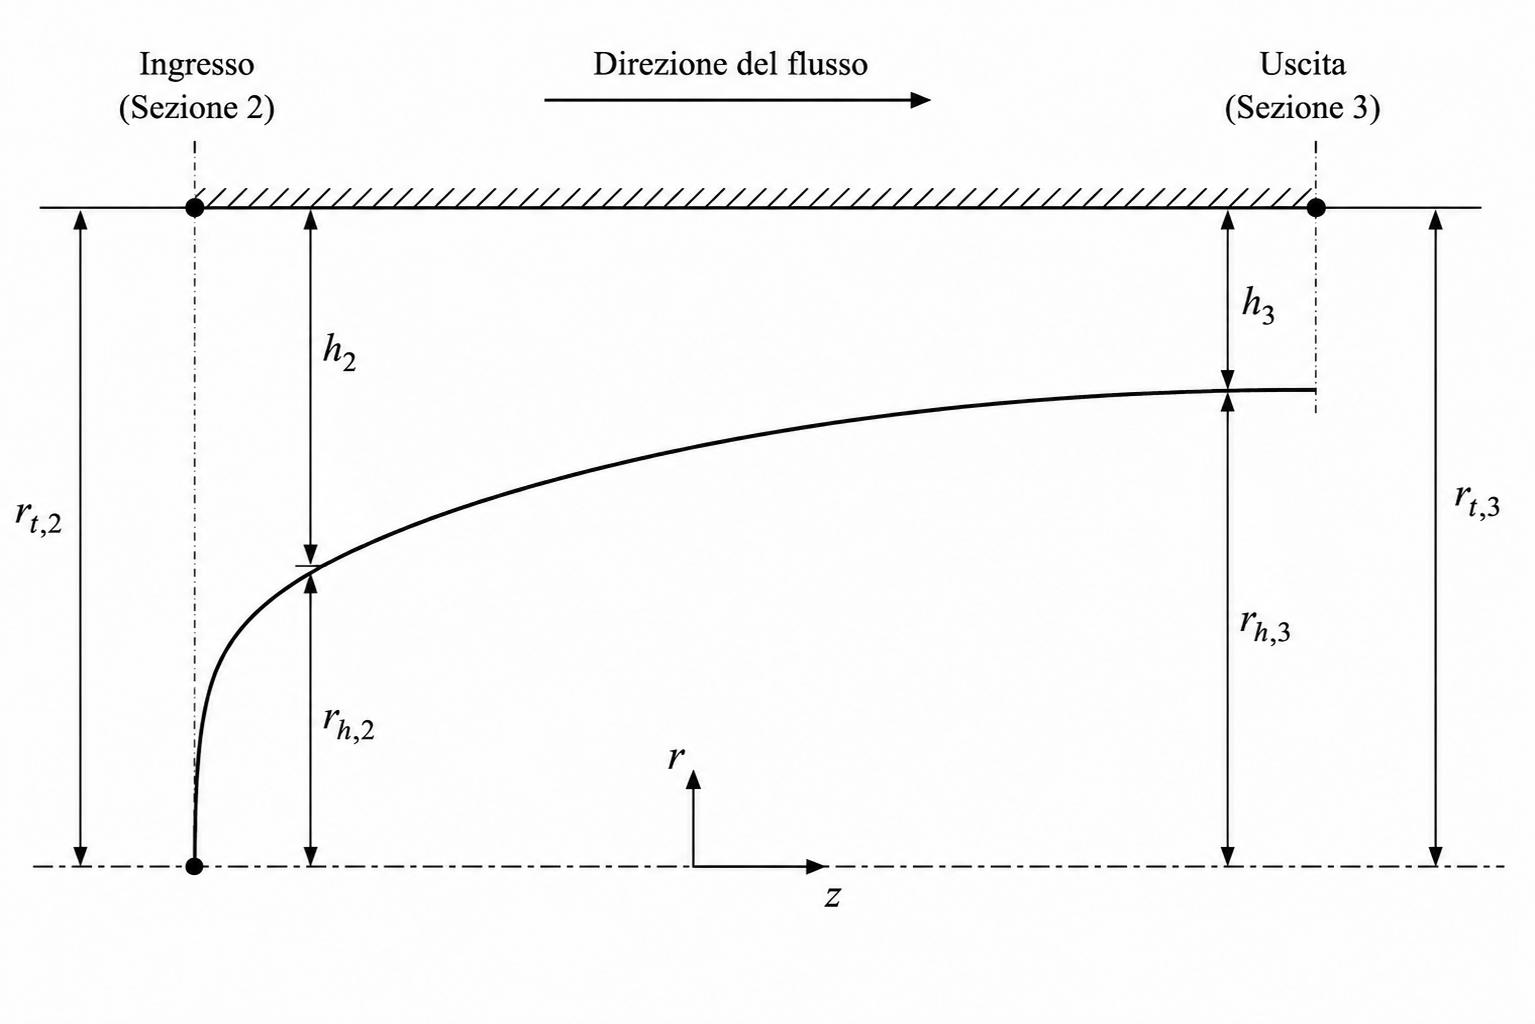
\includegraphics[width=\linewidth]
        {Graphics/turbogetto/compressore/schema_compressore.png}
    \end{minipage}%
    \hfill
    %---------------------------------------------------------
    % MINIPAGE DESTRA: tabella
    %---------------------------------------------------------
\begin{minipage}[c]{0.34\textwidth}
    \centering

    \footnotesize
    \fontsize{11pt}{11pt}\selectfont
    \renewcommand{\arraystretch}{1}
    \setlength{\tabcolsep}{3pt}

    \begin{tabular}{lc}
        \toprule
        \textbf{Dimensione} & \textbf{Valore [mm]} \\
        \midrule

        $r_{t,2}$ & 500 \\
        $r_{h,2}$ & 250 \\
        $r_{m,2}$ & 375 \\
        $h_2$     & 250 \\

        \addlinespace

        $r_{t,3}$ & 500 \\
        $r_{h,3}$ & 470 \\
        $r_{m,3}$ & 485 \\
        $h_3$     & 30.0 \\

        \bottomrule
    \end{tabular}
\end{minipage}

    \caption{Geometria del canale anulare del compressore e principali
    dimensioni nelle sezioni di ingresso e di uscita.}
    \label{fig:geometria_compressore}
\end{figure}

%---------------------------------
\begin{table}[H]
    \centering
    \caption{Principali parametri del compressore.}
    \label{tab:compressore_risultati}
    \fontsize{11pt}{11pt}\selectfont
    \renewcommand{\arraystretch}{1}
    \begin{tabular}{lcccc}
        \toprule
        \textbf{Grandezza} &
        \textbf{Simbolo} &
        \textbf{Valore} &
        \textbf{Limite} &
        \textbf{Unità} \\
        \midrule

        Rapporto di compressione
        & $\pi_c$ & 13.8 & -- & -- \\

        Rendimento politropico
        & $\eta_{p,c}$ & 0.900 & -- & -- \\

        Rendimento isoentropico
        & $\eta_c$ & 0.859 & -- & -- \\

        Potenza assorbita
        & $\dot{L}_c$ & 10.8 & -- & MW \\

        Velocità periferica di punta
        & $U_{tip}$ & 330 & -- & m/s \\

        Numero di stadi
        & $N_{\mathrm{stadi}}$ & 13 & $<15$ & -- \\

        Numero di pale rotoriche
        & $N_{\mathrm{pale,r}}$ & 50 & -- & -- \\

        \midrule

        Mach relativo massimo
        & $M_{\mathrm{rel}}$ & 0.946 & $<1$ & -- \\

        Fattore di De Haller
        & $DeHaller$ & 0.730 & $>0.72$ & -- \\

        Coefficiente di carico
        & $C_p$ & 0.468 & $<0.5$ & -- \\

        Coefficiente di diffusione rotore
        & $D_r$ & 0.443 & $<0.6$ & -- \\

        Coefficiente di diffusione statore
        & $D_s$ & 0.383 & $<0.6$ & -- \\

        Grado di reazione
        & $R$ & 0.796 & -- & -- \\

        \bottomrule
    \end{tabular}
\end{table}



%----------------
I risultati ottenuti rispettano i vincoli aerodinamici e geometrici
introdotti nell'ottimizzazione, in modo particolare il compressore presenta un rapporto di compressione
$\pi_c=13.8$ e richiede 13 stadi.
























\section{Camera di Combustione}
\label{sec:camera}

Il dimensionamento è stato condotto nel punto di progetto turbogetto ($M=0.85$, $h=12000$ m), a partire dalle condizioni totali in uscita dal diffusore ($P_{03}'$, $T_{03}'$, $M_{03}'$) e imponendo come vincolo la temperatura totale di uscita $T_{04}$ (TIT), scelta contenuta per limitare il carico termico sulla turbina.

\paragraph{Diffusore di raccordo compressore-camera.}
A monte della camera è presente un breve diffusore anulare, che decelera il flusso in uscita dal compressore ($M_3\approx0.32$) fino al Mach di ingresso in camera imposto per contenere le perdite nel combustore ($M_{3.5}=0.2$). La temperatura totale si conserva (trasformazione adiabatica), mentre la pressione totale subisce una perdita contenuta ($\pi_d=0.97$). Il semi-angolo di apertura è stato limitato a $\theta=3^\circ$ per evitare distacchi dello strato limite. Le condizioni risultanti in uscita ($P_{03}'=394.2$ kPa, $T_{03}'=570.9$ K) costituiscono l'ingresso del modello di camera descritto di seguit.

\paragraph{Scelte di progettazione.}
Si è adottato JP-7 ($f_{st}=0.068$) per l'elevata stabilità termica alle alte temperature di parete e per il potere calorifico, caratteristiche che lo rendono standard per motori a ciclo combinato operanti anche nel regime supersonico del secondo punto di progetto. La camera è di tipo anulare a doppia zona: una zona primaria (\textit{liner}), in cui l'aria ``calda'' reagisce fino a $T_{comb}$, prossima alle condizioni stechiometriche, e una zona di diluizione in cui l'aria ``fredda'' by-passata viene miscelata adiabaticamente per riportare la temperatura al valore target $T_{04}$. La doppia zona è necessaria perché una combustione condotta direttamente al rapporto aria/combustibile globale risulterebbe troppo povera per una fiamma stabile; l'architettura riproduce quella dei combustori anulari aeronautici reali, disaccoppiando stabilità di fiamma e temperatura di uscita.

%-----------------------------------------
\cici{
\begin{table}[H]
    \centering
    \caption{Vincoli di progetto della camera di combustione e relativo significato fisico.}
    \label{tab:vincoli_camera}
    \fontsize{11pt}{11pt}\selectfont
    \renewcommand{\arraystretch}{1}
    \begin{tabular}
        \toprule
        \textbf{Vincolo} & \textbf{Significato fisico} \\
        \midrule
        $T_{comb}$ & Fissa $\phi = f_{liner}/f_{st}$ nella zona primaria; mantiene $\phi$ in un intorno fisicamente sostenibile, evitando fiamma instabile o vicina allo spegnimento. \\
        $\Delta P/q_{ref}=\text{cost}$ & Fissa $A_{ref}$ tramite la correlazione classica per combustori anulari; governa il compromesso tra ingombro trasversale e perdita di pressione totale. \\
        $I = \dot{Q}/(V\,P_{03}')$ & Fissa il volume di reazione $V$ e quindi $L_c$; il vincolo di chiusura è $t_{res}=L_c/U_{liner} > 8$ ms (tempo caratteristico di combustione del JP-7), a garanzia della completezza della reazione. \\
        \bottomrule
    \end{tabular}
\end{table}
}
%------------------------------------
\begin{table}[H]
    \centering
    \fontsize{11pt}{11pt}\selectfont
    \renewcommand{\arraystretch}{1}
    \caption{Parametri principali della camera di combustione.}
    \label{tab:camera_combustione}
    \begin{tabular}{lccc}
        \toprule
        \textbf{Grandezza} & \textbf{Simbolo} & \textbf{Valore} & \textbf{Unità} \\
        \midrule
        Temperatura zona primaria & $T_{comb}$ & 2300 & K \\
        Rapporto di equivalenza & $\phi$ & 0.757 & -- \\
        Portata combustibile & $\dot{m}_{comb}$ & 0.938 & kg/s \\
        Sezione di riferimento & $A_{ref}$ & 0.396 & m$^2$ \\
        Volume camera & $V$ & 0.507 & m$^3$ \\
        Lunghezza assiale & $L_c$ & 1.28 & m \\
        Tempo di residenza & $t_{res}$ & 40.0 & ms \\
        Perdita di pressione & $\Delta P/P_{03}'$ & 6.00 & \% \\
        Temperatura in camera di combustione & $T_{04}$ & 1620 & K \\ 
        \bottomrule
    \end{tabular}
\end{table}
Il dimensionamento della camera è stato condotto imponendo la temperatura
$T_{comb}$ nella zona primaria, dalla quale viene determinato il rapporto
di equivalenza $\phi=f_{liner}/f_{st}$. La sezione di riferimento
$A_{ref}$ è stata ricavata imponendo un valore costante del rapporto
$\Delta P/q_{ref}$, mentre il volume di reazione $V$ è stato determinato
mediante il parametro di intensità di combustione
$I=\dot{Q}/(VP_{03}')$. L'intensità di combustione è stata fissata pari a
\(I=20\,\mathrm{MW/(m^3\,bar)}\), valore corrispondente al limite inferiore
dell'intervallo \(20{-}50\,\mathrm{MW/(m^3\,bar)}\) indicato in letteratura
per camere di combustione per i motori aeronautici \cite{cohen2001gas}.
La lunghezza della camera risultante è stata infine
verificata imponendo un tempo di residenza $t_{res}>8$ ms.

I risultati principali sono riassunti in Tabella~\ref{tab:camera_combustione}. I valori ottenuti rientrano nei range tipici per combustori anulari aeronautici: $\phi=0.757$ è moderatamente magro ma stabile (range tipico $[0.6,\,1.2]$); $t_{res}=40.0$ ms offre un margine ampio rispetto al vincolo minimo di 8 ms, indicando che la zona di reazione non opera al limite della propria capacità di completare la combustione. La perdita di pressione (6\%) si colloca nella parte alta del range tipico 3--6\%, compensata da una sezione frontale contenuta ($A_{ref}=0.396$ m$^2$, ben al di sotto del vincolo di 0.8 m$^2$) complessiva del propulsore.
\label{sec:turbina}
\hspace{2cm}
\section{Turbina}

%\subsection{Rafreddamento}
La turbina rappresenta uno dei componenti più sollecitati dal punto di vista termomeccanico. Le alte temperature raggiunte in camera di combustione impongono il raffreddamento delle palette, in modo particolare nei primi stadi dello statore e del rotore, esposti alle condizioni più critiche.  Poiché la modellazione  dell'intero sistema di raffreddamento richiederebbe una trattazione indipendente, nel modello sono state introdotte alcune semplificazioni:
\begin{itemize}
    \item L'aria spillata viene stimata in base alla temperatura di combustione, ricavata mediante i grafici riportati nella bibliografia~\cite{slidesRobertoAndriani} e descritti nell'Appendice~\ref{ap:appendixA}.
    \item Una miscelazione adiabatica nella turbina, tra l'aria appena uscita dalla camera di combustione e l'aria  spillata dal compressore.
    \item Si è introdotto un singolo rendimento meccanico per tenere conto della potenza richiesta da sistemi elettrici, idraulici e attriti meccanici ($\eta_m = 0.95$). 
\end{itemize}

\subsection{Primo stadio della turbina}
L'analisi è focalizzata sul singolo primo stadio i cui parametri operativi sono successivamente estesi per determinare il numero di stadi complessivi della turbina. 
Nello sviluppo del modello si assumono le seguenti ipotesi semplificative:
\begin{itemize}
    \item Viene trascurata ogni perdita di pressione nello statore e rotore. Di conseguenza, la componente assiale della velocità viene considerata costante ($v_{z} = \text{cost}$).
    \item Il raggio medio della turbina coincide con il raggio medio dell'ultimo stadio del compressore.
    \item Turbogetto a singolo albero, pertanto la velocità angolare della turbina coincide con quella del compressore. 
\end{itemize}

\textbf{Statore}\\
Per il calcolo dei parametri dello statore, il fluido viene fatto espandere fino al raggiungimento del blocco sonico, ossia una condizione di Mach pari a 1 all'uscita dello statore. La velocità in ingresso allo statore pari alla velocità di ingresso e uscita della turbina, è assunta completamente assiale con un numero di Mach all'ingresso pari a 0,5. Tale valore è stato scelto sulla base di un'analisi della variazione del numero di Mach in ingresso (Figura \ref{fig:turb:machRelativoEMachIngresso}) e delle dimensioni del turbogetto. In particolare,  un numero di Mach inferiore comporterebbe un aumento della potenza generata dallo stadio. Tuttavia, questa scelta determinerebbe anche un incremento dell'area di uscita della turbina e, di conseguenza, delle sue dimensioni. Poiché il guadagno in termini di potenza risulta limitato, si è ritenuto opportuno adottare un valore di Mach in ingresso pari a 0,5 minimizzando l'area di ingresso e di uscita della turbina.

\textbf{Rotore}\\
La velocità relativa in uscita dal rotore viene imposta in un intervallo di numero di Mach compreso tra 0,8 e 0,9. In particolare,un aumento del numero di Mach in uscita comporta un incremento del lavoro prodotto dallo stadio come mostrato nella Figura \ref{fig:turb:machRelativoEMachIngresso}. Inoltre, all'aumentare del numero di Mach in uscita si registra anche un leggero incremento del rendimento dello stadio. Pertanto si è scelto un numero di Mach pari a 0,9. 

\textbf{Triangoli di velocità}

Il lavoro estratto dal rotore può essere di tipo ad azione o a reazione. In particolare, la ripartizione dell'accelerazione del fluido, dipende dal grado di reazione dello stadio.



% Pala con profilo NACA 2412 approssimato.
% Uso: \DrawBlade{x}{y}{angolo}


% ============================================================
% PARAMETRI MODIFICABILI
% ============================================================
\def\Denoms{150}

% Triangolo di ingresso
\def\OoneX{0}
\def\OoneY{0}

% Estremo di V1
% VoneX diverso da OoneX rende V1 inclinato.
\def\VoneX{618/\Denoms}
\def\VoneY{-385/\Denoms}

% Estremo di W1
\def\WoneX{298/\Denoms}
\def\WoneY{-385/\Denoms}

% Valori visualizzati
\def\VoneValue{728}
\def\WoneValue{386}
\def\UoneValue{320}

% Angoli visualizzati
\pgfmathsetmacro{\AlphaOneValue}{round(10*atan2(abs(\VoneX),abs(\VoneY)))/10}
\def\BetaOneValue{58.1}

% Triangolo di uscita
\def\OtwoX{9}
\def\OtwoY{-5.7}

% Estremo di V2
\def\VtwoX{-124/\Denoms+\OtwoX}
\def\VtwoY{-385/\Denoms+\OtwoY}

% Estremo di W2
\def\WtwoX{-444/\Denoms+\OtwoX}
\def\WtwoY{-385/\Denoms+\OtwoY}

% Valori visualizzati
\def\VtwoValue{404}
\def\WtwoValue{587}
\def\UtwoValue{320}

% Angoli visualizzati

%\pgfmathsetmacro{\AlphaTwoValue}{round(10*atan2(abs(\VtwoX-\OtwoX),abs(\VtwoY-\OtwoY)))/10}

\def\AlphaTwoValue{17.9}

\def\BetaTwoValue{40}

% Pale
\def\BladeAngle{-105}
\def\BladeY{-3.3}

\begin{figure}[H]
\centering
\begin{tikzpicture}[
  scale=0.8,
  font=\fontsize{7}{8}\selectfont,
  absolute/.style={ultra thick,cyan!80!blue,-{Stealth[length=3mm,width=2.2mm]}},
  relative/.style={ultra thick,orange,-{Stealth[length=3mm,width=2.2mm]}},
  peripheral/.style={ultra thick,green!70!black,-{Stealth[length=3mm,width=2.2mm]}},
  reference/.style={dashed,gray!60,thin},
  velocitylabel/.style={text=black,fill=white,inner sep=2pt},
  angletext/.style={text=black,fill=white,inner sep=1pt}
]

% ============================================================
% TRIANGOLO DI INGRESSO
% ============================================================

\coordinate (O1) at (\OoneX,\OoneY);
\coordinate (V1) at (\VoneX,\VoneY);
\coordinate (W1) at (\WoneX,\WoneY);
\coordinate (VerticalOne) at (\OoneX,-3.1);

% Linea verticale di riferimento
\draw[reference] (O1) -- (VerticalOne);

% Vettore V1
\draw[absolute]
  (O1) -- (V1)
  node[velocitylabel,midway,right=10pt]
  {$v_{1.5}=\VoneValue\,\mathrm{m/s}$};

% Vettore W1
\draw[relative]
  (O1) -- (W1)
  node[velocitylabel,midway,below left=1pt]
  {$w_{1.5}=\WoneValue\,\mathrm{m/s}$};

% Vettore U1
\draw[peripheral]
  (W1) -- (V1)
  node[velocitylabel,midway,below=5pt]
  {$U=\UoneValue\,\mathrm{m/s}$};

% Arco beta 1
%\pic[
%  draw,
%  angle radius=1.25cm
%]
%  {angle=VerticalOne--O1--W1};
%
%\node[angletext]
%  at (0.70,-1.15)
%  {$\beta_1=\BetaOneValue^\circ$};

% Arco alpha 1
% Diventa visibile quando V1 viene inclinato.
\pic[
  draw,
  angle radius=0.72cm
]
  {angle=VerticalOne--O1--V1};

\node[angletext]
  at (1.6,0)
  {$\alpha_{1.5} = \pgfmathprintnumber[fixed, precision=1]{\AlphaOneValue}^\circ$}


% ============================================================
% PALE NACA
% ============================================================

\DrawBlade{0}{\BladeY}{\BladeAngle}
\DrawBlade{2}{\BladeY}{\BladeAngle}
\DrawBlade{4}{\BladeY}{\BladeAngle}
\DrawBlade{6}{\BladeY}{\BladeAngle}
\DrawBlade{8}{\BladeY}{\BladeAngle}




% ============================================================
% FRECCIA DI ROTAZIONE
% ============================================================

\node[
  single arrow,
  draw=green!70!black,
  fill=white,
  thick,
  minimum height=1cm,
  minimum width=0.5cm,
  single arrow head extend=0.1cm,
  anchor=east,
  shape border rotate=0
]
  (rotor) at (-0.5,-4.3) {};

\node[
  left=4pt,
  align=center,
  font=\sffamily\scriptsize
]
  at (rotor.west)
  {\textbf{Rotazione}\\\textbf{del rotore}};


% ============================================================
% PIANO DI USCITA
% ============================================================

\draw[gray!65,thin]
  (-1,-5.45) -- (9,-5.45);

\node[below,text=gray!65,font=\scriptsize]
  at (3.2,-5.45)
  {piano di uscita del rotore};


% ============================================================
% TRIANGOLO DI USCITA
% ============================================================

\coordinate (O2) at (\OtwoX,\OtwoY);
\coordinate (V2) at (\VtwoX,\VtwoY);
\coordinate (W2) at (\WtwoX,\WtwoY);
\coordinate (VerticalTwo) at (\OtwoX,-8.3);

% Linea verticale di riferimento
\draw[reference] (O2) -- (VerticalTwo);

% Vettore V2
\draw[absolute]
  (O2) -- (V2)
  node[velocitylabel, midway, below right=8pt, xshift=-4pt]
  {$v_2=\VtwoValue\,\mathrm{m/s}$};

% Vettore W2
\draw[relative]
  (O2) -- (W2)
  node[velocitylabel,midway,left=10pt]
  {$w_2=\WtwoValue\,\mathrm{m/s}$};

% Vettore U2
\draw[peripheral]
  (W2) -- (V2)
  node[velocitylabel,midway,below=8pt]
  {$U=\UtwoValue\,\mathrm{m/s}$};

% Arco alpha 2
\pic[
  draw,
  angle radius=0.5cm
]
  {angle=V2--O2--VerticalTwo};

\node[angletext]
  at (10.1,-6.3)
  {$\alpha_2=\AlphaTwoValue^\circ$};

% Arco beta 2
%\pic[
%  draw,
%  angle radius=1.55cm
%]
%  {angle=VerticalTwo--O2--W2};
%
%\node[angletext]
%  at (9.80,-6.65)
%  {$\beta_2=\BetaTwoValue^\circ$};
\draw[->, thick] (9,0) -- (10.5, 0) node[right] {$\theta$};
% Asse theta (verticale)
\draw[->, thick] (9,0) -- (9, -1.5) node[below] {$z$};
% Origine
\fill (0,0) circle (1.5pt);

  
\end{tikzpicture}
    \caption{Diagramma dei triangoli di velocità all'ingresso (1.5) e all'uscita (2) del rotore.}
    \label{fig:turb:triangoli}
\end{figure}




L'angolo di uscita dallo statore ($\alpha_1$ nella Figura \ref{fig:turb:triangoli}) non coincide con l'angolo ottimo, come mostrato nell'appendice \ref{ap:appendixB}. Sebbene il valore calcolato disti dall'ottimo teorico, questa differenza è dovuta al vincolo di progetto di tenere la velocità assiale costante. 

\begin{table}[H]
\centering
\caption{Principali parametri della turbina e grandezze fluidodinamiche
del singolo stadio.}
\label{tab:turbina:tabellaDati}

\scriptsize
\renewcommand{\arraystretch}{0.95}
\fontsize{11pt}{11pt}\selectfont
\renewcommand{\arraystretch}{1}
\begin{tabular*}{0.92\textwidth}
{@{\extracolsep{\fill}} lcc lcc}
    \toprule

    \multicolumn{6}{c}{\textbf{Parametri della turbina}} \\
    \midrule

    \textbf{Parametro} & \textbf{Valore} & \textbf{Unità} &
    \textbf{Parametro} & \textbf{Valore} & \textbf{Unità} \\
    \midrule

    $\dot{L}$            & 11.3  & MW
    & $\eta_t$           & 0.912 & -- \\

    $N_{\mathrm{stadi}}$ & 2     & --
    & $P_{05}$           & 112   & kPa \\

    $T_{05}$             & 1240  & K
    & $\beta$            & 0.303   & -- \\

    $A_{4}$             & 0.113   & m$^2$
    & $A_{5}$           & 0.329   & m$^2$ \\

    $x_{\mathrm{spill}}$ & 9.49  & \%
    &                    &       & \\

    \midrule

    \multicolumn{6}{c}{\textbf{Primo stadio}} \\
    \midrule

    $\dot{L}_{\mathrm{st}}$ & 8.09 & MW
    & $v_z$                   & 385  & m/s \\

    $R$                     & 0.229 & --
    & $U$                   & 320  & m/s \\


    \midrule
\end{tabular*}

% ============================================================
% STATORE / ROTORE con colonne simmetriche
% ============================================================

\begin{tabular*}{0.92\textwidth}{
@{\extracolsep{\fill}}
l
>{\centering\arraybackslash}p{0.12\textwidth}
>{\centering\arraybackslash}p{0.12\textwidth}
>{\centering\arraybackslash}p{0.12\textwidth}
>{\centering\arraybackslash}p{0.12\textwidth}
c
}
    \textbf{Grandezza} &
    \multicolumn{2}{c}{\textbf{Statore}} &
    \multicolumn{2}{c}{\textbf{Rotore}} &
    \textbf{Unità} \\

    \cmidrule(lr){2-3}
    \cmidrule(lr){4-5}

    &
    \textbf{In} &
    \textbf{Out} &
    \textbf{In} &
    \textbf{Out} &
    \\

    $T_0$
    & 1620 & 1620
    & 1530 & 1320
    & K \\

    $P_0$
    & 371 & 371
    & 371 & 152
    & kPa \\

    $v$
    & 385 & 728
    & 728 & 404
    & m/s \\

    $v_{\theta}$
    & 0.00 & 618
    & 618 & -124
    & m/s \\

    $w_{\theta}$
    & 0 & 298
    & 298 & -444
    & m/s \\

    $A$
    & 0.113 & 0.0843
    & 0.171 & 0.331
    & m$^2$ \\

    \bottomrule
\end{tabular*}

\end{table}


Nella Tabella \ref{tab:turbina:tabellaDati}, la temperatura totale in uscita dallo statore non combacia con la temperatura totale all'ingresso dello rotore. Questa discrepanza è dovuta al raffreddamento della turbina. Per permettere questo calcolo si è assunto di effettuare una miscelazione adiabatica a pressione costante subito dopo l'uscita dallo statore con tutta l'area di raffreddamento, senza alcuna variazione di velocità. Pertanto anche l'area di ingresso della turbina comprende solo i gas combusti in uscita dalla camera di combustione. 


\begin{figure}[H]
\centering
\begin{minipage}[c]{0.58\textwidth}
\begin{tikzpicture}[
    scale=0.8,
    thick,
    >=Stealth,
    font=\sffamily
]

    % --- Asse di rotazione e Linea Media ---
    % Asse di rotazione
    \draw[dash dot, thin] (1,0) -- (9,0);
    
    % Linea media di flusso (r_m1)
    \draw[dashed, thin] (1,2.7) -- (8.0,2.7);

    % --- Albero / Rotore (Shaft) ---
    \draw[thick] (3.2,0) ellipse (0.35cm and 0.5cm);
    \draw[thick] (3.2,-0.5) -- (7.2,-0.5);
    \draw[thick] (3.2,0.5) -- (4.1,0.5);
    \draw[thick] (7.2,-0.5) arc (-90:90:0.35cm and 0.5cm);
    \draw[thick] (4.7,0.5) -- (5.9,0.5);
    \draw[thick] (6.5,0.5) -- (7.2,0.5);

    

    % --- Palettature (N1, R1, N2, R2) ---

    % N1 (Statore 1)
    \draw[thick] (3.2,3.5) -- (3.2,1.84) -- (3.8,1.72) -- (3.8,3.7) -- cycle;
    \node at (3.5, 2.7) {N1};

    % R1 (Rotore 1)
    \draw[thick]  (4.1,0.5) -- (4.1,3.7) -- (4.7,3.9) -- (4.7,0.5);
    \draw[thick]  (4.1,1.66) -- (4.7,1.54);
    \node at (4.4, 2.7) {R1};

    % N2 (Statore 2)
    \draw[thick] (5.0,4.1) -- (5.0,1.48) -- (5.6,1.36) -- (5.6,4.3) -- cycle;
    \node at (5.3, 2.7) {N2};

    % R2 (Rotore 2)
    \draw[thick] (5.9,0.5) -- (5.9,4.3) -- (6.5,4.5) -- (6.5,0.5);
    \draw[thick]  (5.9,1.26) -- (6.5,1.12);
    \node at (6.2, 2.7) {R2};

    % --- Inviluppo Superiore (Cassa / Tip) ---
    \draw[ultra thick] (3.1,3.47) -- (6.6,4.63);

    % --- Cerchi Stazioni (4, 2, 5) ---
    % Stazione 4 (Ingresso)
    \node[draw, circle, inner sep=1pt, minimum size=5mm] at (3.2, 4) {\small 4};
    
    % Stazione 2 (Tra N1 e R1)
    %\node[draw, circle, inner sep=1pt, minimum size=5mm] at (3.95, 4.25) {\small 2};
    
    % Stazione 5 (Uscita R2)
    \node[draw, circle, inner sep=1pt, minimum size=5mm] at (6.5, 5.05) {\small 5};

    % --- Quote a Sinistra (Sezione d'Ingresso / Stazione 2) ---
    % Linee di riferimento orizzontali
    \draw[thin] (1, 3.7) -- (4.1, 3.7);
    \draw[thin] (2.3, 1.66) -- (4.1, 1.66);

    % Frecce verticali
    \draw[<->] (1.1, 0) -- (1.1, 3.7) node[midway, fill=white] {$r_{t1.5}$};
    \draw[<->] (1.7, 0) -- (1.7, 2.7) node[midway, fill=white] {$r_{m}$};
    \draw[<->] (2.3, 0) -- (2.3, 1.66) node[midway, fill=white] {$r_{h1.5}$};
    \draw[<->] (2.5, 1.66) -- (2.5, 3.7) node[midway, fill=white] {$h_{1.5}$};

    % --- Quote a Destra (Sezione d'Uscita / Stazione 5) ---
    % Linee di riferimento orizzontali
    \draw[thin] (6.5, 4.5) -- (9, 4.5);
    \draw[thin] (6.5, 1.12) -- (8.7, 1.12);

    % Frecce verticali
    \draw[<->] (7.3, 1.12) -- (7.3, 4.5) node[midway, fill=white] {$h_5$};
    \draw[<->] (8.1, 0) -- (8.1, 1.12) node[midway, fill=white] {$r_{h5}$};
    \draw[<->] (8.9, 0) -- (8.9, 4.5) node[midway, fill=white] {$r_{t5}$};

    % --- Equazione in basso centrata ---

\end{tikzpicture}
\end{minipage}%
\hfill
  % --- MINIPAGE DI DESTRA: Tabella ---
\begin{minipage}[c]{0.38\textwidth}
    \raggedleft
    
    \fontsize{11pt}{11pt}\selectfont
    \renewcommand{\arraystretch}{1}
    \setlength{\tabcolsep}{3.5pt}

    \begin{tabular}{cc}
        \toprule
        \textbf{Dimensione} & \textbf{Valore [mm]} \\
        \midrule

        $r_{t2}$ & 513  \\
        $r_{h2}$ & 457  \\
        $h_2$    & 56.3 \\

        \addlinespace

        $r_{t5}$ & 539 \\
        $r_{h5}$ & 431 \\
        $h_5$    & 108 \\

        \bottomrule
    \end{tabular}

    \label{tab:dati_turbina}
\end{minipage}
  \caption{Raggi di mozzo e di punta del rotore del primo stadio e dell'uscita della turbina, con indicazione dei valori e della relativa rappresentazione grafica.}
\end{figure}











\cici{ % togliere se si vuole vedere la tabella

\begin{table}[H]
\centering
\caption{Principali parametri della turbina e grandezze fluidodinamiche
del singolo stadio.}
\label{tab:turbina:tabellaDati}

\footnotesize
\setlength{\tabcolsep}{4pt}

% ============================================================
% TABELLA SINISTRA
% ============================================================
\begin{minipage}[t]{0.39\textwidth}
    \centering

    \begin{tabular}{lcc}
        \toprule
        \textbf{Parametro} &
        \textbf{Valore} &
        \textbf{Unità} \\
        \midrule

        \multicolumn{3}{l}{\textbf{Turbina globale}} \\
        \midrule

        $\dot{L}$            
        & 1200  & MW \\

        $\eta_N$             
        & 0.907 & -- \\

        $N_{\mathrm{stadi}}$ 
        & 2     & -- \\

        $P_{05}$             
        & 137   & kPa \\

        $T_{05}$             
        & 1110  & K \\

        $\beta$              
        & 2.2   & -- \\

        $A_{04}$             
        & 0.7   & m$^2$ \\

        $A_{05}$             
        & 0.3   & m$^2$ \\

        $x_{\mathrm{spill}}$ 
        & 8.89  & \% \\

        \addlinespace[2pt]

        \multicolumn{3}{l}{\textbf{Singolo stadio}} \\
        \midrule

        $\dot{L}_{\mathrm{st}}$
        & 1288 & MW \\

        $\eta_{\mathrm{iso}}$
        & 0.90 & -- \\

        $R$
        & 0.23 & -- \\

        $U$
        & 350 & m/s \\

        $v_z$
        & 200 & m/s \\

        \bottomrule
    \end{tabular}

\end{minipage}
\hfill
% ============================================================
% TABELLA DESTRA
% ============================================================
\begin{minipage}[t]{0.57\textwidth}
    \centering

    \begin{tabular}{lcccc}
        \toprule
        &
        \multicolumn{2}{c}{\textbf{Statore}} &
        \multicolumn{2}{c}{\textbf{Rotore}} \\
        \cmidrule(lr){2-3}
        \cmidrule(lr){4-5}

        \textbf{Grandezza} &
        \textbf{In} &
        \textbf{Out} &
        \textbf{In} &
        \textbf{Out} \\
        \midrule

        $T_0$ [K]
        & 1288 & 1288 & 1288 & 1243 \\

        $P_0$ [kPa]
        & 283 & 283 & 283 & 180 \\

        $v$ [m/s]
        & 701 & 701 & 701 & 340 \\

        $v_{\theta}$ [m/s]
        & 634 & 634 & 634 & -163 \\

        $w_{\theta}$ [m/s]
        & 300 & 300 & 300 & -463 \\

        $A$ [m$^2$]
        & 0.5 & 0.5 & 0.5 & 0.5 \\

        \bottomrule
    \end{tabular}

\end{minipage}

\end{table}


} %% togliere se si vuole vedere la tabella con \cici
\section{Ugello}
\label{sec:turboUgello}

% VERSIONE COMPRESSA
%------------------------------------------------
L'espansione dei gas combusti è affidata a un ugello convergente-divergente,
assunto operante in condizioni di espansione ottima e modellato con rendimento
$\eta_n=0.95$. La presenza del postbruciatore, inattivo durante il
funzionamento subsonico del turbogetto, è considerata mediante una perdita
di pressione totale $\pi_{ab}=0.98$.

Le aree di gola e di efflusso sono state dimensionate imponendo la condizione
di adattamento $P_e=P_{amb}$. Poiché le condizioni operative differiscono
tra turbogetto e ramjet, è stata prevista una geometria variabile dell'ugello,
in grado di modificare entrambe le sezioni caratteristiche. Il procedimento
di calcolo è riportato in Appendice~\ref{appB:ugello}.



%---------------------------------------

%L'ugello è l'ultimo componente del motore e ha il compito di espandere i gas combusti in modo da generare una spinta che possa essere utilizzata dal velivolo.

%Volendo massimizzare le prestazioni, viene preso in considerazione l'utilizzo di un ugello convergente-divergente. Per semplificare la trattazione del componente si considera di essere in un caso di espansione ottima. Inoltre, si suppone di avere un componente non isentropico con rendimento \(\eta_n=0.95\).

%A causa della presenza di un postbruciatore (che nella fase di volo subsonico rimane spento), i gas in uscita dalla turbina subiranno una perdita di carico \(\pi_{ab}=0.98\).

%Note le pressioni, ed una volta ricavata la differenza di temperatura attraverso il nozzle pressure ratio (NPR) totale è possibile ottenere un valore per la velocità in uscita la quale permette di calcolare l'ingombro delle sezioni di gola e di efflusso.
%Il valore delle aree non è stato considerato fisso per entrambe le modalità di funzionamento in quanto viene considerato l'utilizzo di un sistema a geometria variabile in modo da garantire un'alta flessibilità di utilizzo nei vari regimi di volo.

\begin{table}[H]
    \centering

    \caption{Valori ottenuti}
    \label{tab:my_table}

    \fontsize{11pt}{11pt}\selectfont
    \renewcommand{\arraystretch}{1}
    \setlength{\tabcolsep}{3.5pt}

    \begin{tabular}{cllc}
        \toprule
        \textbf{Grandezza} & 
        \textbf{Simbolo} & 
        \textbf{Valore} & 
        \textbf{Unità di misura} \\
        \midrule

        Pressione totale in uscita     & $P_{06}$ & $98.9$  & \text{kPa} \\
        Temperatura totale in uscita   & $T_{06}$ & $1240$  & \text{K} \\
        Mach di efflusso               & $M_{06}$ & $1.74$  & -- \\
        Velocità di efflusso           & $V_e$    & $978$   & \text{m/s} \\
        Area di gola                   & $A^\star$& $0.274$  & $\text{m}^2$ \\
        Area di efflusso               & $A_e$    & $0.385$  & $\text{m}^2$ \\

        \bottomrule
    \end{tabular}
\end{table}
\label{sec:turbina}
\hspace{2cm}
\section{Prestazioni}



\begin{figure}[H]
    \centering

    \begin{minipage}[c]{0.62\linewidth}
        \centering
        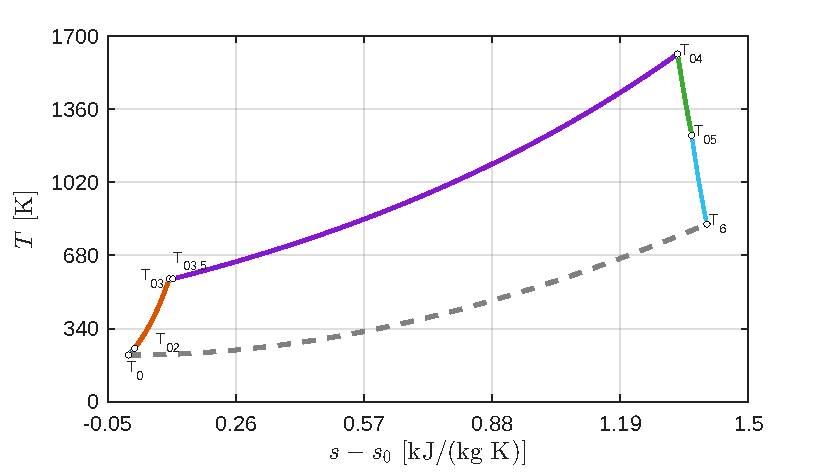
\includegraphics[width=\linewidth]
        {Graphics/turbogetto/prestazioni/ciclo.pdf}
        \caption{Rappresentazione del ciclo termodinamico del turbogetto.}
        \label{fig:prestazione:ciclo}
    \end{minipage}
    \hfill
\begin{minipage}[c]{0.34\linewidth}
    \centering

    \captionof{table}{Pressioni e temperature nei punti del ciclo.}
    \label{tab:pressioni}

    \fontsize{11pt}{11pt}\selectfont
    \renewcommand{\arraystretch}{1}
    \setlength{\tabcolsep}{3.5pt}

    \begin{tabular}{ccc}
        \toprule
        \textbf{Punto} & \textbf{$P$ [kPa]} & \textbf{$T$ [K]} \\
        \midrule
        $0$    & 19.2 & 216  \\
        $02$   & 29.4 & 248  \\
        $03$   & 406  & 571  \\
        $03.5$ & 394  & 571  \\
        $04$   & 371  & 1620 \\
        $05$   & 112  & 1240 \\
        $6$    & 19.2 & 825  \\
        \bottomrule
    \end{tabular}
\end{minipage}

\end{figure}

I principali risultati prestazionali ottenuti nel punto di progetto sono
riportati in Tabella~\ref{tab:prestazioni}.

\begin{table}[H]
\centering
\caption{Prestazioni principali del turbogetto, calcolate secondo la
procedura riportata in Appendice~\ref{appB:prestazioni}.}
\label{tab:prestazioni}
\fontsize{11pt}{11pt}\selectfont
\renewcommand{\arraystretch}{1}
\begin{tabular}{lrl}
\toprule
\textbf{Parametro} & \textbf{Valore} & \textbf{Unità} \\
\midrule
Spinta                    & 25.0  & kN \\
Spinta specifica          & 754 & m/s \\
TSFC                      & 0.135 & kg/(N$\cdot$h) \\
Rendimento propulsivo     & 41.2 & \% \\
Rendimento termodinamico  & 37.4 & \% \\
Rendimento globale        & 15.4 & \% \\
\bottomrule
\end{tabular}
\end{table}

La scelta di massimizzare la spinta specifica conduce a un valore di TSFC
superiore a quello di turbogetti ottimizzati prevalentemente sul consumo,
per i quali possono essere raggiunti valori inferiori a
$0.11\ \mathrm{kg/(N\,h)}$ \cite{Useller1954J71A2}. Tale risultato è
coerente con l'elevata temperatura di combustione adottata, che incrementa
la velocità di efflusso e quindi la spinta specifica, penalizzando al tempo
stesso il rendimento propulsivo \cite{slidesRobertoAndriani}.

\begin{table}[H]
\centering
\fontsize{11pt}{11pt}\selectfont
\renewcommand{\arraystretch}{1}
\caption{Portate massiche del turbogetto nel punto di progetto.}
\label{tab:mass}
\begin{tabular}{lrl}
\toprule
\textbf{Parametro} & \textbf{Valore} & \textbf{Unità} \\
\midrule
$\dot{m}_{\text{aria}}$         & 33.1 & kg/s \\
$\dot{m}_{\text{spillata}}$     & 3.23  & kg/s \\
$\dot{m}_{\text{combustibile}}$ & 0.938  & kg/s \\
$\dot{m}_{\text{totale}}$       & 34.1 & kg/s \\
\bottomrule
\end{tabular}
\end{table}

La portata d'aria richiesta risulta pari a $33.1\ \mathrm{kg/s}$, valore
ottenuto dall'ottimizzazione per soddisfare il requisito di spinta
contenendo al tempo stesso le dimensioni del propulsore. Di tale portata,
$3.23\ \mathrm{kg/s}$ vengono spillati dal compressore per il raffreddamento
della turbina, mentre la portata di combustibile risulta limitata a
$0.938\ \mathrm{kg/s}$.

Il modello introduce alcune semplificazioni, in particolare nella
modellazione della combustione e del raffreddamento della turbina, che
possono influenzare la stima delle prestazioni globali. La configurazione
ottenuta rispetta comunque i vincoli imposti durante l'ottimizzazione e
presenta dimensioni contenute, con raggio massimo all'ingresso della
turbina pari a $539\ \mathrm{mm}$. L'elevata spinta specifica favorisce
quindi una configurazione compatta, facilitando l'integrazione con il
ramjet nel sistema propulsivo complessivo.


































%----------------------------------------------------------------------------------------------------------------------------


%Risultano esserci inoltre alcune inefficienze e semplificazioni che dovrebbero essere prese in considerazione in caso di sviluppi futuri e che dovrebbero essere modificate. In particolare l'angolo $\alpha$ ottimo non verificato per la turbina, dovuto all'ipotesi di tenere la velocità assiale costante.  Il raffreddamento della turbina, che presenta notevoli approssimazioni su tutto il sistema coinvolto, per semplicità non vengono discussi spillamenti extra per sottosistemi. (possiamo mettere anche il fatto che si posso aggiungere molti piu vincoli nel ottimizzazione)




\label{ch:chapter_three}%
\chapter{Ramjet}

%\newpage
\label{sec:presa_ramjet}
\section{Presa d'Aria Supersonica}

% VERSIONE ACCORCIATA
La presa d'aria del ramjet è stata dimensionata nel punto di progetto
($M_0=3.5$, $h=25000$ m) con l'obiettivo di decelerare il flusso fino a
condizioni compatibili con la combustione, massimizzando il recupero di
pressione totale e contenendo al tempo stesso l'ingombro del componente.

\paragraph{Architettura: presa a compressione esterna multirampa.}
È stata adottata una configurazione a compressione esterna su tre rampe,
ciascuna generatrice di un urto obliquo, seguite da un urto normale
terminale che porta il flusso a condizioni subsoniche. Tale architettura
è stata scelta per limitare le elevate perdite di pressione totale che,
a $M_0=3.5$, caratterizzerebbero una decelerazione mediante un singolo
urto normale. La configurazione a tre rampe rappresenta quindi un
compromesso tra recupero di pressione totale, complessità geometrica e
ingombro della presa. Il flusso è stato modellato come adiabatico e non
viscoso, assumendo $T_0=\mathrm{cost}$ e considerando esclusivamente le
perdite di pressione totale associate agli urti, trascurando gli effetti
viscosi e di strato limite sulle rampe.

\paragraph{Ottimizzazione degli urti.}
Definito il numero di rampe, la deflessione complessiva è stata ripartita
secondo il criterio di Oswatitsch. A parità di condizioni iniziali, il
recupero di pressione totale viene massimizzato distribuendo la
compressione tra urti di uguale intensità. Nel modello è stato quindi
imposto lo stesso rapporto di pressione statica attraverso i tre urti
obliqui e tale rapporto è stato determinato mediante la massimizzazione
del recupero di pressione totale complessivo. Ne risultano deflessioni
progressivamente crescenti, pari a $11.8^\circ$, $14.4^\circ$ e
$17.7^\circ$.

A valle del terzo urto il flusso permane supersonico; è stato quindi
introdotto un urto normale terminale per raggiungere condizioni
subsoniche. Questa soluzione comporta un'ulteriore perdita di pressione
totale, ma permette di limitare il numero di rampe e di ottenere una
configurazione geometricamente più compatta.

\paragraph{Dimensionamento geometrico.}
La geometria è stata costruita a partire dalla condizione teorica di
\textit{shock-on-lip}, facendo convergere gli urti verso il labbro della
presa. Rispetto alla configurazione ideale è stato tuttavia introdotto un
margine longitudinale $\Delta s$, arretrando il cowl rispetto al punto
teorico di convergenza. Tale margine è stato introdotto per rendere la
geometria meno sensibile alle variazioni del numero di Mach rispetto al
punto di progetto, che modificano l'inclinazione e quindi la posizione
degli urti. L'area di cattura $A_{\mathrm{catt}}$ è stata invece
determinata dalla portata d'aria richiesta dal ramjet mediante
l'equazione di continuità.

 Il procedimento di calcolo,
il confronto tra differenti numeri di urti e il dimensionamento
geometrico completo sono riportati in Appendice~\ref{app:presa_ramjet}.

La configurazione ottenuta presenta un recupero di pressione totale
$\pi_{\mathrm{tot}}=0.731$ e un'efficienza adiabatica
$\eta_d=0.879$. L'urto normale terminale porta il flusso a
$M_2=0.72$: tale valore, pur essendo subsonico, risulta ancora elevato
per l'ingresso nella camera di combustione e richiede pertanto
un'ulteriore diffusione subsonica a valle della presa.




% ============================================================
% PRESA D'ARIA TBCC - MACH 3.5
% ============================================================


% ============================================================
% 1. PARAMETRI PRINCIPALI
% ============================================================

% Dati ramjet.presaAria
\def\hCatt{1.1005}
\def\LSuper{2.2532}

\def\LRampaOneTwo{1.4907}
\def\LRampaTwoThree{0.7145}
\def\LRampaThreeFour{0.4435}

\def\wCatt{2.2011}

% Valori MATLAB
\def\deltaOneRaw{0.2057}
\def\deltaTwoRaw{0.2521}
\def\deltaThreeRaw{0.3093}

\def\thetaOneRaw{0.4544}
\def\thetaTwoRaw{0.5811}
\def\thetaThreeRaw{0.8046}

% Mach
\def\Mzero{3.5}

% Aree
\def\AtwoRam{0.5273}

% ATTENZIONE:
% sostituire col vero valore di motore.presaAria.A2
\def\AtwoTurbo{0.5273}

% Scala globale
\def\UnitScale{2.45}



% ============================================================
% 2. POSIZIONI MODIFICABILI DELLE SCRITTE
% ============================================================
%
% DX > 0  -> destra
% DX < 0  -> sinistra
%
% DY > 0  -> alto
% DY < 0  -> basso
% ============================================================

% theta 1
\def\ThetaOneDX{0.09}
\def\ThetaOneDY{0.18}

% delta 1
\def\DeltaOneDX{-0.03}
\def\DeltaOneDY{0.13}

% theta 2
\def\ThetaTwoDX{0.1}
\def\ThetaTwoDY{0.05}

% delta 2
\def\DeltaTwoDX{-0.02}
\def\DeltaTwoDY{0.14}

% theta 3
\def\ThetaThreeDX{0.1}
\def\ThetaThreeDY{0.1}

% delta 3
\def\DeltaThreeDX{-0.02}
\def\DeltaThreeDY{0.19}

% Shock point
\def\ShockTextDX{-0.5}
\def\ShockTextDY{0}

% Offset
\def\OffsetTextDX{-0.2}
\def\OffsetTextDY{-0.08}

% Ingresso compressore
\def\CompressorTextDX{-0.71}
\def\CompressorTextDY{-0.1}

% Mach
\def\MachTextDX{-0.10}
\def\MachTextDY{0.00}

% Post combustore
\def\PostTextDX{-0.2}
\def\PostTextDY{0.00}

% Etichette B C D E
\def\BTextDX{-0.05}
\def\BTextDY{0.05}

\def\CTextDX{0.00}
\def\CTextDY{0.06}

\def\DTextDX{0.00}
\def\DTextDY{0.06}

\def\ETextDX{0.00}
\def\ETextDY{0.06}



% ============================================================
% 3. CONVERSIONE ANGOLI
% ============================================================

\pgfmathsetmacro{\deltaOne}{deg(\deltaOneRaw)}
\pgfmathsetmacro{\deltaTwo}{deg(\deltaTwoRaw)}
\pgfmathsetmacro{\deltaThree}{deg(\deltaThreeRaw)}

\pgfmathsetmacro{\thetaOne}{deg(\thetaOneRaw)}
\pgfmathsetmacro{\thetaTwo}{deg(\thetaTwoRaw)}
\pgfmathsetmacro{\thetaThree}{deg(\thetaThreeRaw)}

\pgfmathsetmacro{\thetaFlow}{
    \deltaOne+\deltaTwo+\deltaThree
}



% ============================================================
% 4. AREE E ALTEZZE
% ============================================================

\pgfmathsetmacro{\hComp}{
    2*sqrt(\AtwoTurbo/pi)
}



% ============================================================
% 5. COORDINATE RAMPE
% ============================================================

\pgfmathsetmacro{\xB}{0}
\pgfmathsetmacro{\yB}{\hCatt}

\pgfmathsetmacro{\xC}{
    \xB+\LRampaOneTwo*cos(\deltaOne)
}

\pgfmathsetmacro{\yC}{
    \yB-\LRampaOneTwo*sin(\deltaOne)
}

\pgfmathsetmacro{\xD}{
    \xC+\LRampaTwoThree*cos(\deltaOne+\deltaTwo)
}

\pgfmathsetmacro{\yD}{
    \yC-\LRampaTwoThree*sin(\deltaOne+\deltaTwo)
}

\pgfmathsetmacro{\xE}{
    \xD+\LRampaThreeFour*cos(\thetaFlow)
}

\pgfmathsetmacro{\yE}{
    \yD-\LRampaThreeFour*sin(\thetaFlow)
}



% ============================================================
% 6. SHOCK POINT
% ============================================================

\pgfmathsetmacro{\xShock}{\LSuper}
\pgfmathsetmacro{\yShock}{0}



% ============================================================
% 7. OFFSET LABBRO
% ============================================================

\pgfmathsetmacro{\offsetLabbro}{
    0.05*\LSuper
}

\pgfmathsetmacro{\xLip}{
    \xShock+\offsetLabbro*cos(\thetaFlow)
}

\pgfmathsetmacro{\yLip}{
    \yShock-\offsetLabbro*sin(\thetaFlow)
}



% ============================================================
% 8. GEOMETRIA INTERNA
% ============================================================

\pgfmathsetmacro{\xHinge}{
    \xE+0.80*\LSuper
}

\pgfmathsetmacro{\xMax}{
    \xHinge+0.25*\LSuper
}

\pgfmathsetmacro{\yFloor}{
    -0.45*\hCatt
}

\pgfmathsetmacro{\yHinge}{
    \yFloor+sqrt(\AtwoRam/pi)
}

\pgfmathsetmacro{\yRoof}{
    \yHinge+\hComp
}



% ============================================================
% 9. PUNTI BEZIER - TETTO
% ============================================================

\pgfmathsetmacro{\RoofPoneX}{
    \xE+0.5*(\xHinge-\xE)
}

\pgfmathsetmacro{\RoofPoneY}{
    \yE
}

\pgfmathsetmacro{\RoofPtwoX}{
    \xHinge-0.2*(\xHinge-\xE)
}

\pgfmathsetmacro{\RoofPtwoY}{
    \yRoof
}



% ============================================================
% 10. PUNTI BEZIER - PARATIA MOBILE
% ============================================================

\pgfmathsetmacro{\dxFlap}{
    \xHinge-\xE
}

\pgfmathsetmacro{\FlapPoneX}{
    \xE+0.35*\dxFlap
}

\pgfmathsetmacro{\FlapPoneY}{
    \yE-0.25*\dxFlap*tan(\thetaFlow)
}

\pgfmathsetmacro{\FlapPtwoX}{
    \xHinge-0.35*\dxFlap
}

\pgfmathsetmacro{\FlapPtwoY}{
    \yHinge
}



% ============================================================
% 11. PUNTI BEZIER - PAVIMENTO RAMJET
% ============================================================

\pgfmathsetmacro{\dxFloor}{
    \xHinge-\xLip
}

\pgfmathsetmacro{\FloorPoneX}{
    \xLip+0.35*\dxFloor
}

\pgfmathsetmacro{\FloorPoneY}{
    \yLip-0.25*\dxFloor*tan(\thetaFlow)
}

\pgfmathsetmacro{\FloorPtwoX}{
    \xHinge-0.35*\dxFloor
}

\pgfmathsetmacro{\FloorPtwoY}{
    \yFloor
}



% ============================================================
% 12. ANGOLI ONDE D'URTO
% ============================================================

\pgfmathsetmacro{\aShockOne}{
    atan2(\yShock-\yB,\xShock-\xB)
}

\pgfmathsetmacro{\aShockTwo}{
    atan2(\yShock-\yC,\xShock-\xC)
}

\pgfmathsetmacro{\aShockThree}{
    atan2(\yShock-\yD,\xShock-\xD)
}



% ============================================================
% 13. DIREZIONE RAMPE
% ============================================================

\pgfmathsetmacro{\aRampOne}{
    -\deltaOne
}

\pgfmathsetmacro{\aRampTwo}{
    -(\deltaOne+\deltaTwo)
}

\pgfmathsetmacro{\aRampThree}{
    -(\deltaOne+\deltaTwo+\deltaThree)
}



% ============================================================
% 14. PARAMETRI ARCHI E FRECCE
% ============================================================

\pgfmathsetmacro{\rTheta}{
    0.16*\LSuper
}

\pgfmathsetmacro{\rDelta}{
    0.08*\LSuper
}

\pgfmathsetmacro{\Ldash}{
    0.20*\LSuper
}

\pgfmathsetmacro{\Larr}{
    0.08*\LSuper
}



% ============================================================
% 15. POSIZIONI FRECCE FLUSSO
% ============================================================

% Rampa 1
\pgfmathsetmacro{\mXOne}{
    (\xB+\xC)/2
}

\pgfmathsetmacro{\yShockOne}{
    \yB+
    (\yShock-\yB)/(\xShock-\xB)*
    (\mXOne-\xB)
}

\pgfmathsetmacro{\mYOne}{
    ((\yB+\yC)/2+\yShockOne)/2
}


% Rampa 2
\pgfmathsetmacro{\mXTwo}{
    (\xC+\xD)/2
}

\pgfmathsetmacro{\yShockTwo}{
    \yC+
    (\yShock-\yC)/(\xShock-\xC)*
    (\mXTwo-\xC)
}

\pgfmathsetmacro{\mYTwo}{
    ((\yC+\yD)/2+\yShockTwo)/2
}


% Rampa 3
\pgfmathsetmacro{\mXThree}{
    (\xD+\xE)/2
}

\pgfmathsetmacro{\yShockThree}{
    \yD+
    (\yShock-\yD)/(\xShock-\xD)*
    (\mXThree-\xD)
}

\pgfmathsetmacro{\mYThree}{
    ((\yD+\yE)/2+\yShockThree)/2
}


% Flusso interno
\pgfmathsetmacro{\mXFour}{
    (\xE+\xLip)/2+
    0.04*\LSuper*cos(\aRampThree)
}

\pgfmathsetmacro{\mYFour}{
    (\yE+\yLip)/2+
    0.04*\LSuper*sin(\aRampThree)
}



% ============================================================
% 16. FIGURA
% ============================================================

\begin{figure}[htbp]

\centering

\begin{tikzpicture}[
    scale = 0.8,
     transform shape,
    x=\UnitScale cm,
    y=\UnitScale cm,
    line cap=round,
    line join=round,
    font=\scriptsize,
    >={Stealth[length=2.6mm,width=2mm]}
]


% ============================================================
% FUSOLIERA SUPERIORE
% ============================================================

\draw[
    black,
    line width=0.8pt
]
({-0.15*\LSuper},\hCatt)
--
(\xMax,\hCatt);



% ============================================================
% RAMPE
% ============================================================

\draw[
    black,
    line width=1.3pt
]
(\xB,\yB)
--
(\xC,\yC)
--
(\xD,\yD)
--
(\xE,\yE);



% ============================================================
% ONDE D'URTO
% ============================================================

\draw[
    red,
    line width=1.3pt
]
(\xB,\yB)
--
(\xShock,\yShock);

\draw[
    red,
    line width=1.3pt
]
(\xC,\yC)
--
(\xShock,\yShock);

\draw[
    red,
    line width=1.3pt
]
(\xD,\yD)
--
(\xShock,\yShock);

\draw[
    red,
    line width=1.3pt
]
(\xE,\yE)
--
(\xShock,\yShock);



% ============================================================
% SHOCK POINT
% ============================================================

\fill[
    red
]
(\xShock,\yShock)
circle[radius=2pt];


\node[
    red,
    font=\bfseries\scriptsize
]
at
(
    {\xShock+\ShockTextDX},
    {\yShock+\ShockTextDY}
)
{
    Shock point
};



% ============================================================
% OFFSET LABBRO
% ============================================================

\draw[
    green!60!black,
    line width=3pt
]
(\xShock,\yShock)
--
(\xLip,\yLip);


\node[
    green!55!black,
    font=\bfseries\scriptsize
]
at
(
    {\xLip+\OffsetTextDX},
    {\yLip+\OffsetTextDY}
)
{
    Offset
};



% ============================================================
% TETTO TURBOGETTO
% ============================================================

\draw[
    black,
    line width=1.3pt
]
(\xE,\yE)
..
controls
    (\RoofPoneX,\RoofPoneY)
and
    (\RoofPtwoX,\RoofPtwoY)
..
(\xHinge,\yRoof)
--
(\xMax,\yRoof);



% ============================================================
% PARATIA MOBILE
% ============================================================

\draw[
    orange!85!black,
    line width=2.2pt
]
(\xE,\yE)
..
controls
    (\FlapPoneX,\FlapPoneY)
and
    (\FlapPtwoX,\FlapPtwoY)
..
(\xHinge,\yHinge);


\filldraw[
    fill=orange!85!black,
    draw=black,
    line width=0.5pt
]
(\xHinge,\yHinge)
circle[radius=2pt];



% ============================================================
% PAVIMENTO RAMJET
% ============================================================

\draw[
    black,
    line width=1.3pt
]
(\xLip,\yLip)
..
controls
    (\FloorPoneX,\FloorPoneY)
and
    (\FloorPtwoX,\FloorPtwoY)
..
(\xHinge,\yFloor)
--
(\xMax,\yFloor);



% ============================================================
% LINEA DIVISORIA
% ============================================================

\draw[
    black,
    line width=1.3pt
]
(\xHinge,\yHinge)
--
(\xMax,\yHinge);



% ============================================================
% INGRESSO COMPRESSORE
% ============================================================

\draw[
    magenta,
    line width=3pt
]
(\xMax,\yHinge)
--
(\xMax,\yRoof);


\node[
    magenta,
    font=\bfseries\scriptsize
]
at
(
    {\xMax+\CompressorTextDX},
    {(\yHinge+\yRoof)/2+\CompressorTextDY}
)
{
    Ingresso compressore
};



% ============================================================
% FRECCIA MACH
% ============================================================

\draw[
    ->,
    black,
    line width=1.5pt
]
({-0.1*\LSuper},{0.5*\hCatt})
--
({0.05*\LSuper},{0.5*\hCatt});


\node[
    font=\bfseries
]
at
(
    {-0.28*\LSuper+\MachTextDX},
    {0.5*\hCatt+\MachTextDY}
)
{
    $M_0=\Mzero$
};



% ============================================================
% POST COMBUSTORE
% ============================================================

\node[
    gray,
    font=\itshape\scriptsize
]
at
(
    {
      \xHinge
      +0.5*(\xMax-\xHinge)
      +\PostTextDX
    },
    {
      \yFloor
      +0.5*(\yHinge-\yFloor)
      +\PostTextDY
    }
)
{
    Post combustore $\rightarrow$
};



% ============================================================
% RAMPA 1
% ============================================================

\draw[
    dashed,
    cyan!70!blue,
    line width=0.8pt
]
(\xB,\yB)
--
++(\Ldash,0);


\draw[
    cyan!70!blue,
    line width=1pt
]
(\xB,\yB)
++(0:\rTheta)
arc[
    start angle=0,
    end angle=\aShockOne,
    radius=\rTheta
];


\draw[
    red,
    line width=1pt
]
(\xB,\yB)
++(0:\rDelta)
arc[
    start angle=0,
    end angle=\aRampOne,
    radius=\rDelta
];


\node[
    cyan!70!blue,
    font=\bfseries
]
at
(
    {
      \xB
      +1.12*\rTheta*cos(\aShockOne/2)
      +\ThetaOneDX
    },
    {
      \yB
      +1.12*\rTheta*sin(\aShockOne/2)
      +\ThetaOneDY
    }
)
{
    $\theta_1$
};


\node[
    red,
    font=\bfseries
]
at
(
    {
      \xB
      +1.30*\rDelta*cos(\aRampOne/2)
      +\DeltaOneDX
    },
    {
      \yB
      +1.30*\rDelta*sin(\aRampOne/2)
      +\DeltaOneDY
    }
)
{
    $\delta_1$
};


\draw[
    ->,
    black,
    line width=1.5pt
]
(
    {\mXOne-\Larr*cos(\aRampOne)/2+0.7},
    {\mYOne-\Larr*sin(\aRampOne)/2-0.35}
)
--
(
    {\mXOne+\Larr*cos(\aRampOne)/2+0.7},
    {\mYOne+\Larr*sin(\aRampOne)/2-0.35}
);



% ============================================================
% RAMPA 2
% ============================================================

\draw[
    dashed,
    cyan!70!blue,
    line width=0.8pt
]
(\xC,\yC)
--
++(\Ldash,0);


\draw[
    cyan!70!blue,
    line width=1pt
]
(\xC,\yC)
++(0:\rTheta)
arc[
    start angle=0,
    end angle=\aShockTwo,
    radius=\rTheta
];


\draw[
    red,
    line width=1pt
]
(\xC,\yC)
++(0:\rDelta)
arc[
    start angle=0,
    end angle=\aRampTwo,
    radius=\rDelta
];


\node[
    cyan!70!blue,
    font=\bfseries
]
at
(
    {
      \xC
      +1.12*\rTheta*cos(\aShockTwo/2)
      +\ThetaTwoDX
    },
    {
      \yC
      +1.12*\rTheta*sin(\aShockTwo/2)
      +\ThetaTwoDY
    }
)
{
    $\theta_2$
};


\node[
    red,
    font=\bfseries
]
at
(
    {
      \xC
      +1.30*\rDelta*cos(\aRampTwo/2)
      +\DeltaTwoDX
    },
    {
      \yC
      +1.30*\rDelta*sin(\aRampTwo/2)
      +\DeltaTwoDY
    }
)
{
    $\delta_2$
};


\draw[
    ->,
    black,
    line width=1.5pt
]
(
    {\mXTwo-\Larr*cos(\aRampTwo)/2+0.2},
    {\mYTwo-\Larr*sin(\aRampTwo)/2-0.2}
)
--
(
    {\mXTwo+\Larr*cos(\aRampTwo)/2+0.2},
    {\mYTwo+\Larr*sin(\aRampTwo)/2-0.2}
);



% ============================================================
% RAMPA 3
% ============================================================

\draw[
    dashed,
    cyan!70!blue,
    line width=0.8pt
]
(\xD,\yD)
--
++(\Ldash,0);


\draw[
    cyan!70!blue,
    line width=1pt
]
(\xD,\yD)
++(0:\rTheta)
arc[
    start angle=0,
    end angle=\aShockThree,
    radius=\rTheta
];


\draw[
    red,
    line width=1pt
]
(\xD,\yD)
++(0:\rDelta)
arc[
    start angle=0,
    end angle=\aRampThree,
    radius=\rDelta
];


\node[
    cyan!70!blue,
    font=\bfseries
]
at
(
    {
      \xD
      +1.12*\rTheta*cos(\aShockThree/2)
      +\ThetaThreeDX
    },
    {
      \yD
      +1.12*\rTheta*sin(\aShockThree/2)
      +\ThetaThreeDY
    }
)
{
    $\theta_3$
};


\node[
    red,
    font=\bfseries
]
at
(
    {
      \xD
      +1.30*\rDelta*cos(\aRampThree/2)
      +\DeltaThreeDX
    },
    {
      \yD
      +1.30*\rDelta*sin(\aRampThree/2)
      +\DeltaThreeDY
    }
)
{
    $\delta_3$
};


\draw[
    ->,
    black,
    line width=1.5pt
]
(
    {\mXThree-\Larr*cos(\aRampThree)/2},
    {\mYThree-\Larr*sin(\aRampThree)/2}
)
--
(
    {\mXThree+\Larr*cos(\aRampThree)/2},
    {\mYThree+\Larr*sin(\aRampThree)/2}
);



% ============================================================
% FRECCIA FLUSSO INTERNO
% ============================================================

\draw[
    ->,
    black,
    line width=1.5pt
]
(
    {\mXFour-\Larr*cos(\aRampThree)/2},
    {\mYFour-\Larr*sin(\aRampThree)/2}
)
--
(
    {\mXFour+\Larr*cos(\aRampThree)/2},
    {\mYFour+\Larr*sin(\aRampThree)/2}
);



% ============================================================
% ETICHETTE B C D E
% ============================================================

\node
at
(
    {\xB+\BTextDX},
    {\yB+\BTextDY}
)
{
    $B$
};


\node
at
(
    {\xC+\CTextDX},
    {\yC+\CTextDY}
)
{
    $C$
};


\node
at
(
    {\xD+\DTextDX},
    {\yD+\DTextDY}
)
{
    $D$
};


\node
at
(
    {\xE+\ETextDX},
    {\yE+\ETextDY}
)
{
    $E$
};

%%% lunghezaa


\end{tikzpicture}

\caption{
Presa d'aria TBCC a $M_0=\Mzero$.
}

\end{figure}





\begin{figure}[H]
    \centering

    % --- MINIPAGE DI SINISTRA: IMMAGINE ---
    \begin{minipage}[c]{0.55\textwidth}
        \centering
        % ============================================================
% PRESA D'ARIA TBCC - VERSIONE BIANCO E NERO
% ============================================================


% ============================================================
% 1. PARAMETRI PRINCIPALI
% ============================================================

% Dati reali MATLAB
\def\hCatt{1.1005}
\def\LSuper{2.2532}

\def\LRampaOneTwo{1.4907}
\def\LRampaTwoThree{0.7145}
\def\LRampaThreeFour{0.4435}

% Delta s
\def\DeltaS{0.2253}

% Angoli MATLAB originali
% Servono SOLO per costruire la geometria.
% Non vengono visualizzati.
\def\deltaOneRaw{0.2057}
\def\deltaTwoRaw{0.2521}
\def\deltaThreeRaw{0.3093}

% Mach
\def\Mzero{3.5}

% Aree
\def\AtwoRam{0.5273}

% Sostituire con motore.presaAria.A2 se hai il valore preciso
\def\AtwoTurbo{0.5273}

% Scala globale
\def\UnitScale{2.45}



% ============================================================
% 2. POSIZIONI MODIFICABILI DELLE SCRITTE
% ============================================================
%
% DX positivo = destra
% DX negativo = sinistra
%
% DY positivo = alto
% DY negativo = basso
% ============================================================

% Shock point
\def\ShockTextDX{-0.20}
\def\ShockTextDY{-0.08}

% Mach
\def\MachTextDX{-0.10}
\def\MachTextDY{0.00}

% Compressore
\def\CompressorTextDX{-0.15}
\def\CompressorTextDY{0.00}

% Post combustore
\def\PostTextDX{0.00}
\def\PostTextDY{0.00}

% B
\def\BTextDX{-0.04}
\def\BTextDY{0.06}

% C
\def\CTextDX{0.00}
\def\CTextDY{0.07}

% D
\def\DTextDX{0.00}
\def\DTextDY{0.07}

% E
\def\ETextDX{0.00}
\def\ETextDY{0.07}

% A = Shock point
\def\ATextDX{-0.08}
\def\ATextDY{0.04}

% A' = punto dopo Delta_s
\def\AprimeTextDX{0.05}
\def\AprimeTextDY{0.04}



% ============================================================
% 3. CONVERSIONE ANGOLI
% ============================================================

% I valori MATLAB vengono usati con sin/cos,
% quindi li convertiamo internamente per TikZ.

\pgfmathsetmacro{\deltaOne}{deg(\deltaOneRaw)}
\pgfmathsetmacro{\deltaTwo}{deg(\deltaTwoRaw)}
\pgfmathsetmacro{\deltaThree}{deg(\deltaThreeRaw)}

\pgfmathsetmacro{\thetaFlow}{
    \deltaOne+\deltaTwo+\deltaThree
}



% ============================================================
% 4. ALTEZZA COMPRESSORE
% ============================================================

\pgfmathsetmacro{\hComp}{
    2*sqrt(\AtwoTurbo/pi)
}



% ============================================================
% 5. COORDINATE RAMPE
% ============================================================

% B
\pgfmathsetmacro{\xB}{0}
\pgfmathsetmacro{\yB}{\hCatt}

% C
\pgfmathsetmacro{\xC}{
    \xB+\LRampaOneTwo*cos(\deltaOne)
}

\pgfmathsetmacro{\yC}{
    \yB-\LRampaOneTwo*sin(\deltaOne)
}

% D
\pgfmathsetmacro{\xD}{
    \xC+\LRampaTwoThree*cos(\deltaOne+\deltaTwo)
}

\pgfmathsetmacro{\yD}{
    \yC-\LRampaTwoThree*sin(\deltaOne+\deltaTwo)
}

% E
\pgfmathsetmacro{\xE}{
    \xD+\LRampaThreeFour*cos(\thetaFlow)
}

\pgfmathsetmacro{\yE}{
    \yD-\LRampaThreeFour*sin(\thetaFlow)
}



% ============================================================
% 6. SHOCK POINT = A
% ============================================================

\pgfmathsetmacro{\xShock}{\LSuper}
\pgfmathsetmacro{\yShock}{0}



% ============================================================
% 7. PUNTO A' DOPO DELTA S
% ============================================================

% Delta_s è interpretato come distanza orizzontale,
% come nella figura di riferimento.

\pgfmathsetmacro{\xLip}{
    \xShock+\DeltaS
}

% Il punto continua nella direzione della terza rampa
\pgfmathsetmacro{\yLip}{
    \yShock-\DeltaS*tan(\thetaFlow)
}



% ============================================================
% 8. GEOMETRIA INTERNA
% ============================================================

\pgfmathsetmacro{\xHinge}{
    \xE+0.80*\LSuper
}

\pgfmathsetmacro{\xMax}{
    \xHinge+0.25*\LSuper
}

\pgfmathsetmacro{\yFloor}{
    -0.45*\hCatt
}

\pgfmathsetmacro{\yHinge}{
    \yFloor+sqrt(\AtwoRam/pi)
}

\pgfmathsetmacro{\yRoof}{
    \yHinge+\hComp
}



% ============================================================
% 9. BEZIER - TETTO
% ============================================================

\pgfmathsetmacro{\RoofPoneX}{
    \xE+0.5*(\xHinge-\xE)
}

\pgfmathsetmacro{\RoofPoneY}{
    \yE
}

\pgfmathsetmacro{\RoofPtwoX}{
    \xHinge-0.2*(\xHinge-\xE)
}

\pgfmathsetmacro{\RoofPtwoY}{
    \yRoof
}



% ============================================================
% 10. BEZIER - PARATIA
% ============================================================

\pgfmathsetmacro{\dxFlap}{
    \xHinge-\xE
}

\pgfmathsetmacro{\FlapPoneX}{
    \xE+0.35*\dxFlap
}

\pgfmathsetmacro{\FlapPoneY}{
    \yE-0.25*\dxFlap*tan(\thetaFlow)
}

\pgfmathsetmacro{\FlapPtwoX}{
    \xHinge-0.35*\dxFlap
}

\pgfmathsetmacro{\FlapPtwoY}{
    \yHinge
}



% ============================================================
% 11. BEZIER - PAVIMENTO
% ============================================================

\pgfmathsetmacro{\dxFloor}{
    \xHinge-\xLip
}

\pgfmathsetmacro{\FloorPoneX}{
    \xLip+0.35*\dxFloor
}

\pgfmathsetmacro{\FloorPoneY}{
    \yLip-0.25*\dxFloor*tan(\thetaFlow)
}

\pgfmathsetmacro{\FloorPtwoX}{
    \xHinge-0.35*\dxFloor
}

\pgfmathsetmacro{\FloorPtwoY}{
    \yFloor
}



% ============================================================
% 12. FIGURA
% ============================================================


\centering

\begin{tikzpicture}[
    x=\UnitScale cm,
    y=\UnitScale cm,
    line cap=round,
    line join=round,
    font=\scriptsize,
    >={Stealth[length=2.5mm,width=1.8mm]}
]

\clip
  ({-0.42*\LSuper},{\yFloor-0.45})
  rectangle
  ({\xHinge-0.65*\LSuper},{\hCatt+0.15});

% ============================================================
% FUSOLIERA SUPERIORE / REFERENCE AXIS
% ============================================================

\draw[
    black,
    line width=0.9pt
]
({-0.15*\LSuper},\hCatt)
--
(\xMax,\hCatt);





% ============================================================
% RAMPE B-C-D-E
% ============================================================

\draw[
    black,
    line width=1.3pt
]
(\xB,\yB)
--
(\xC,\yC)
--
(\xD,\yD)
--
(\xE,\yE);



% ============================================================
% ONDE D'URTO - TUTTE NERE
% ============================================================

\draw[
    black,
    line width=1.1pt
]
(\xB,\yB)
--
(\xShock,\yShock);


\draw[
    black,
    line width=1.1pt
]
(\xC,\yC)
--
(\xShock,\yShock);


\draw[
    black,
    line width=1.1pt
]
(\xD,\yD)
--
(\xShock,\yShock);


\draw[
    black,
    line width=1.1pt
]
(\xE,\yE)
--
(\xShock,\yShock);



% ============================================================
% SHOCK POINT
% ============================================================




% ============================================================
% TRATTO A -> A'
% ============================================================

\draw[
    black,
    dashed,
    line width=1pt
]
(\xShock,\yShock)
--
(\xLip,\yLip);



% ============================================================
% ETICHETTE A E A'
% ============================================================

\node
at
(
    {\xShock+\ATextDX},
    {\yShock+\ATextDY-0.1}
)
{
    $A$
};


\node
at
(
    {\xLip+\AprimeTextDX},
    {\yLip+\AprimeTextDY}
)
{
    $A'$
};



% ============================================================
% TETTO
% ============================================================

\draw[
    black,
    line width=1.3pt
]
(\xE,\yE)
..
controls
    (\RoofPoneX,\RoofPoneY)
and
    (\RoofPtwoX,\RoofPtwoY)
..
(\xHinge,\yRoof)
--
(\xMax,\yRoof);



% ============================================================
% PARATIA MOBILE
% ============================================================

\draw[
    black,
    line width=1.6pt
]
(\xE,\yE)
..
controls
    (\FlapPoneX,\FlapPoneY)
and
    (\FlapPtwoX,\FlapPtwoY)
..
(\xHinge,\yHinge);


\fill[
    black
]
(\xHinge,\yHinge)
circle[radius=1.8pt];



% ============================================================
% PAVIMENTO
% ============================================================

\draw[
    black,
    line width=1.3pt
]
(\xLip,\yLip)
..
controls
    (\FloorPoneX,\FloorPoneY)
and
    (\FloorPtwoX,\FloorPtwoY)
..
(\xHinge,\yFloor)
--
(\xMax,\yFloor);



% ============================================================
% LINEA DIVISORIA
% ============================================================

\draw[
    black,
    line width=1.2pt
]
(\xHinge,\yHinge)
--
(\xMax,\yHinge);



% ============================================================
% FACCIA COMPRESSORE
% ============================================================

\draw[
    black,
    line width=2.3pt
]
(\xMax,\yHinge)
--
(\xMax,\yRoof);








% ============================================================
% ETICHETTE B C D E
% ============================================================

\node
at
(
    {\xB+\BTextDX},
    {\yB+\BTextDY}
)
{
    $B$
};


\node
at
(
    {\xC+\CTextDX},
    {\yC+\CTextDY}
)
{
    $C$
};


\node
at
(
    {\xD+\DTextDX},
    {\yD+\DTextDY}
)
{
    $D$
};


\node
at
(
    {\xE+\ETextDX},
    {\yE+\ETextDY}
)
{
    $E$
};



% ============================================================
% QUOTA VERTICALE h
% ============================================================

% Posizione della quota
\pgfmathsetmacro{\xHeightDim}{
    -0.38*\LSuper
}

% Linee di estensione
\draw[
    black,
    thin
]
(\xHeightDim,\hCatt)
--
(\xB,\hCatt);


\draw[
    black,
    thin
]
(\xHeightDim,\yShock)
--
(\xShock,\yShock);


% Freccia verticale
\draw[
    <->,
    black,
    line width=0.9pt
]
(\xHeightDim,\yShock)
--
(\xHeightDim,\hCatt);


% Etichetta h
\node[
    rotate=90,
    fill=white,
    inner sep=2pt
]
at
(
    \xHeightDim,
    {(\hCatt+\yShock)/2}
)
{
    $h$
};



% ============================================================
% QUOTA L_SUPER
% ============================================================

\pgfmathsetmacro{\yLsuperDim}{
    \yFloor-0.28
}

% Estensioni verticali
\draw[
    black,
    thin
]
(\xB,\yShock)
--
(\xB,\yLsuperDim);


\draw[
    black,
    thin
]
(\xShock,\yShock)
--
(\xShock,\yLsuperDim);


% Quota
\draw[
    <->,
    black,
    line width=0.9pt
]
(\xB,\yLsuperDim)
--
(\xShock,\yLsuperDim);


\node[
    fill=white,
    inner sep=2pt
]
at
(
    {(\xB+\xShock)/2},
    \yLsuperDim
)
{
    $L_{\mathrm{SUPER}}$
};



% ============================================================
% QUOTA DELTA_S
% ============================================================

\pgfmathsetmacro{\yDeltaDim}{
    \yLsuperDim+0.16
}

% Estensione shock point
\draw[
    black,
    thin
]
(\xShock,\yShock)
--
(\xShock,\yDeltaDim);


% Estensione A'
\draw[
    black,
    thin
]
(\xLip,\yLip)
--
(\xLip,\yDeltaDim);


% Quota Delta_s
\draw[
    <->,
    black,
    line width=0.9pt
]
(\xShock,\yDeltaDim)
--
(\xLip,\yDeltaDim);


\node[
    fill=white,
    inner sep=1pt
]
at
(
    {(\xShock+\xLip)/2},
    \yDeltaDim
)
{
    $\Delta_s$
};


\end{tikzpicture}


\caption{
Schema geometrico della presa d'aria TBCC.}

    \end{minipage}%
    \hfill
    % --- MINIPAGE DI DESTRA: TABELLA ---
    \begin{minipage}[c]{0.44\textwidth}
        \centering


               \captionof{table}{Parametri principali della presa d'aria supersonica del ramjet.}
               
        \scriptsize
        \renewcommand{\arraystretch}{1}
        \setlength{\tabcolsep}{3.5pt}

 
        \fontsize{11pt}{11pt}\selectfont
        \begin{tabular}{lcc}
            \toprule
            \textbf{Parametro} & \textbf{Valore} & \textbf{Unità} \\
            \midrule
            $\delta_1$ & 11.8 & $^\circ$ \\
            $\delta_2$ & 14.4 & $^\circ$ \\
            $\delta_3$ & 17.7 & $^\circ$ \\
            $\theta_1$ & 26.0 & $^\circ$ \\
            $\theta_2$ & 33.3 & $^\circ$ \\
            $\theta_3$ & 46.1 & $^\circ$ \\
            \midrule
            $\pi_{\mathrm{tot}}$ & 0.731 & -- \\
            $\eta_d$             & 0.879 & -- \\
            $M_2$                & 0.720 & -- \\
            $T_{02}$             & 765 & K \\
            $P_{02}$             & 142 & kPa \\
            \midrule
            $A_{\mathrm{catt}}$  & 2.42 & m$^2$ \\
            $A_2$                & 0.526 & m$^2$ \\
            $h_{\mathrm{catt}}$  & 1.10 & m \\
            $L_{\mathrm{super}}$ & 2.25 & m \\
            $\Delta s$           & 0.225 & m \\
            \bottomrule
        \end{tabular}

 
    \label{tab:miei_parametri}

        \label{tab:miei_parametri}
    \end{minipage}

\end{figure}


%-------------------------------------------------------------------------------------------------------------------------------------------------------


























\section{Camera di combustione}
\label{sec:camera_combustione}

La camera di combustione del ramjet coincide con il postbruciatore utilizzato dal motore turbogetto, essendo principalmente utilizzato in regime supersonico, il postbruciatore viene quindi dimensionato in questa modalità

\subsection{Anulus}
 L'anulus è posizionato successivamente alla presa d'aria. Viene modellato come un condotto toroidale esterno al motore turbogetto atto a portare il flusso d'aria all'interno della camera di combustione del ramjet. L'area di uscita la quale viene calcolata imponendo un numero di Mach in uscita \(M_{03}=0.6\) risulta pari a \(A_{out}=0.578\) \(m^{2}\) con raggio \(r_{out}=0.6889\) \(m\).
L'intero sistema viene considerato ideale. Nel dimensionamento si assume che, a valle della turbina, il corpo centrale
si raccordi progressivamente fino a chiudersi, consentendo di modellare il
postbruciatore mediante una sezione circolare piena equivalente.

%aggiungi aree

\subsection{Camera/Postbruciatore}
Per garantire un'adeguata stabilità di fiamma si assume un ulteriore rallentamento dell'aria in ingresso imponendo un numero di Mach pari a \(0.25\) in entrata al postbruciatore. Inoltre viene considerato un valore di bloccaggio \(B=0.25\) per gli stabilizzatori di fiamma, mentre il rapporto lunghezza/diametro è stato fissato a \(L/H=2.8\).
Dato che in questo caso la combustione avviene all'interno del postbruciatore, diversamente dal caso subsonico, la perdita di pressione assume un valore maggiore, ovvero \(\pi_{ab}=0.96\) mentre la temperatura totale raggiunta grazie alla combustione è di \(T_{04}=2100 \text{ K}\).
Dal punto di vista del carburante viene utilizzato lo stesso tipo di carburante usato nel turbogetto (JP-7).

\begin{table}[H]
    \centering
    \fontsize{11pt}{11pt}\selectfont
    \renewcommand{\arraystretch}{1}
    \begin{tabular}{cllc}
         \toprule
         \textbf{Grandezza} & \textbf{Simbolo} & \textbf{Valore} & \textbf{Unità di misura} \\
         \midrule
         Rapporto f & $f$ & $0.0413$ & - \\
         Raggio & $r$ & $0.610$ & \text{m} \\
         Lunghezza & $L$ & $3.42$ & \text{m} \\
         Diametro stabilizzatore di fiamma & $d$ & $0.305$ & \text{m} \\
         Pressione totale in uscita & $P_{04}$ & $137$ & \text{kPa} \\
         \bottomrule
    \end{tabular}
\caption{Valori ottenuti per la camera di combustione/postbruciatore}
\label{tab:camera_combustione ramjet}
\end{table}
%aggiungere disegno
\section{Ugello}
Come nel caso subsonico, è stato inizialmente assunto di essere in un caso di espansione ottima ma in seguito alle prime analisi, a causa di una quota di funzionamento maggiore, l'area di efflusso dell'ugello è risultata troppo alta; è stato quindi considerato un ugello che permette di avere un flusso sottoespanso in uscita.
Il valore di pressione in uscita è stato quindi fissato a \(4\) volte la pressione ambiente a \(h=25 \text{ km}\).
Il resto del dimensionamento è stato poi eseguito con le stesse modalità del caso subsonico.

\begin{table}[H]
    \centering
    \caption{Valori ottenuti per l'ugello}
    \renewcommand{\arraystretch}{1}
    \fontsize{11pt}{11pt}\selectfont

    \begin{tabular}{cllc}
         \toprule
         \textbf{Grandezza} & \textbf{Simbolo} & \textbf{Valore} & \textbf{Unità di misura} \\
         \midrule
         Pressione totale in uscita & $P_{05}$ & $114$ & \text{kPa} \\
         Temperatura totale in uscita & $T_{05}$ & $2100$ & \text{K} \\
         Mach di efflusso & $M_{05}$ & $2.23$ & - \\
         Velocità di efflusso & $V_{e}$ & $1480$ & \text{m/s} \\
         Area di gola & $A^\star$ & $0.891$ & $\text{m}^2$ \\
         Area di efflusso & $A_{e}$ & $1.93$ & $\text{m}^2$ \\
         \bottomrule
    \end{tabular}
\label{tab:ugello_ramjet}
\end{table}
Come detto in precedenza la variazione delle aree di gola e di efflusso è resa possibile grazie ad un sistema di superfici mobili.
%inserire disegno

\label{sec:prestazioni_ramjet}
\hspace{2cm}
\section{Prestazioni}


\begin{figure}[H]
    \centering


    %------------------------------------------------
    % CICLO TERMODINAMICO A SINISTRA
    %------------------------------------------------
    \begin{minipage}[c]{0.64\linewidth}
        \centering
        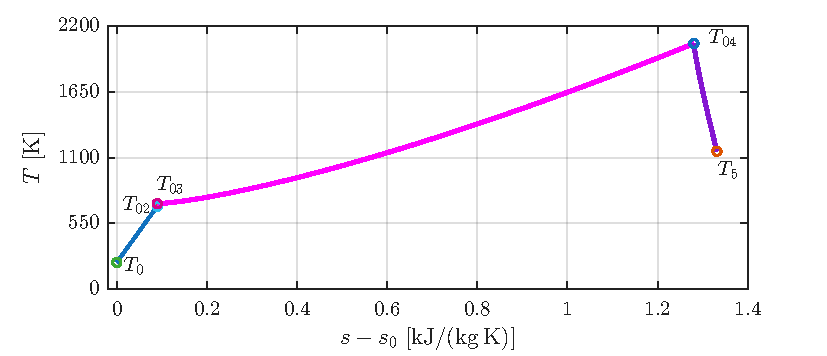
\includegraphics[width=\linewidth]
        {Graphics/ramjet/ciclo_termodinamico_ramjet.pdf}
    \end{minipage}
    \hfill
   %------------------------------------------------
% TABELLA PRESSIONI E TEMPERATURE TOTALI A DESTRA
%------------------------------------------------
\begin{minipage}[c]{0.33\linewidth}
    \centering
    \renewcommand{\arraystretch}{1}
    \fontsize{11pt}{11pt}\selectfont
    \caption{Pressioni e temperature nei punti del ciclo.}
    \begin{tabular}{ccc}
        \toprule
        \textbf{Punto} &
        \textbf{$P$ [kPa]} &
        \textbf{$T$ [K]} \\
        \midrule
        $0$ & 2.55 & 221 \\
        $02$ & 142  & 765 \\
        $03$ & 142  & 765 \\
        $04$ & 137  & 2100 \\
        $5$ & 10.2  & 1150 \\
        \bottomrule
    \end{tabular}
\end{minipage}

\caption{Ciclo termodinamico del ramjet e principali grandezze totali
nelle stazioni del motore.}
\label{fig:prestazioni_ciclo_ramjet}
\end{figure}


\begin{table}[H]
\centering
\renewcommand{\arraystretch}{1}
\fontsize{11pt}{11pt}\selectfont
\caption{Prestazioni principali del ramjet, calcolate secondo la procedura riportata in Appendice~\ref{appC:prestazioni}.}
\label{tab:prestazioni_ramjet}
\begin{tabular}{lrl}
\toprule
\textbf{Parametro} & \textbf{Valore} & \textbf{Unità} \\
\midrule
Spinta                    & 65.0    & kN \\
Spinta specifica         & 643 & m/s \\
TSFC                      & 0.231 & kg/(N$\cdot$h) \\
Rendimento propulsivo     & 81.7  & \% \\
Rendimento termodinamico  & 45.7  & \% \\
Rendimento globale        & 37.4  & \% \\
\bottomrule
\end{tabular}
\end{table}
I principali risultati prestazionali ottenuti nel punto di progetto del ramjet ($M_0=3.5$, $h=25000$ m) sono riportati in Tabella~\ref{tab:prestazioni_ramjet}. Il TSFC ottenuto, pari a $0.231\ \mathrm{kg/(N\,h)}$, risulta inferiore
al limite di $0.278\ \mathrm{kg/(N\,h)}$ imposto dal vincolo di missione
(Appendice~A.3). Il rendimento propulsivo raggiunge l'$81.7\%$: il valore
elevato è associato al ridotto scarto tra la velocità di efflusso e quella
di volo, condizione favorevole alla conversione dell'energia cinetica del
getto in spinta utile. Il rendimento termodinamico risulta pari al
$45.7\%$, mentre dalla combinazione dei due contributi si ottiene un
rendimento globale del $37.4\%$.

\begin{table}[H]
\centering
\renewcommand{\arraystretch}{1}
\fontsize{11pt}{11pt}\selectfont
\caption{Portate massiche del ramjet nel punto di progetto.}
\label{tab:mass_ramjet}
\small
\begin{tabular}{lrl}
\toprule
\textbf{Parametro} & \textbf{Valore} & \textbf{Unità} \\
\midrule
$\dot{m}_{\text{aria}}$         & 101 & kg/s \\
$\dot{m}_{\text{combustibile}}$ & 4.18   & kg/s \\
$\dot{m}_{\text{totale (gas)}}$ & 105 & kg/s \\
\bottomrule
\end{tabular}
\end{table}

Nel punto di progetto il ramjet elabora una portata d'aria di
$101\ \mathrm{kg/s}$, alla quale si aggiungono $4.18\ \mathrm{kg/s}$ di
combustibile, ottenendo una portata complessiva dei gas pari a
$105\ \mathrm{kg/s}$. La maggiore portata d'aria rispetto al turbogetto
è associata alle differenti condizioni operative e, in particolare, alla
maggiore spinta richiesta, pari a $65\ \mathrm{kN}$.

Nel modello del ramjet non sono previsti spillamenti di portata per il
raffreddamento delle turbomacchine, assenti in questa configurazione.
Ciò consente inoltre di adottare una temperatura totale a valle della
combustione pari a $T_{04}=2100\ \mathrm{K}$, superiore alla temperatura
massima imposta nel dimensionamento del turbogetto dalla presenza della
turbina.

Il vincolo geometrico sul diametro di efflusso ($D_{eflusso}<1.6$ m, Tabella 1.4) risulta rispettato, con $D_E=1.57\ \mathrm{m}$: tale vincolo, introdotto proprio per evitare un'espansione completa fino alla pressione ambiente alla quota di crociera (che alle alte quote comporterebbe aree di efflusso eccessive), si riflette in un ugello volutamente sottoespanso, con pressione statica in uscita $P_E=10.2\ \mathrm{kPa}$ superiore alla pressione ambiente $P_0=2.5\ \mathrm{kPa}$ a $25000$ m. Questa scelta comporta una perdita di spinta rispetto all'espansione ottima, compensata dal contenimento dell'ingombro trasversale del propulsore, coerentemente con l'obiettivo di integrazione del ramjet nella configurazione a ciclo variabile con il turbogetto.

\label{ch:chapter_finale}%
\chapter{Conclusioni e sviluppi futuri}

\section{Conclusioni}

La metodologia sviluppata ha consentito di ottenere una configurazione turbogetto--ramjet
compatibile con i requisiti assegnati nei due punti di progetto, integrando nello stesso
processo il dimensionamento termodinamico e geometrico dei principali componenti. Il
turbogetto, dimensionato per una spinta di 25 kN a $M=0.85$ e $h=12$ km, presenta un
TSFC di 0.135 kg/(N$\cdot$h) e un ingombro radiale massimo di 539 mm, con tutti i vincoli
aerodinamici e geometrici imposti in ottimizzazione rispettati. Il ramjet, dimensionato per 65 kN a $M=3.5$ e $h=25$ km,
presenta un TSFC di 0.231 kg/(N$\cdot$h), ampiamente entro il limite di missione, con un
diametro di efflusso di 1.57 m compatibile con il vincolo geometrico imposto.

%---------------------------------------
\section{Sviluppi futuri}

La struttura modulare della procedura di calcolo consente di aumentare
progressivamente il livello di dettaglio del modello, introducendo nuovi
sottosistemi oppure sostituendo quelli esistenti con formulazioni più
accurate. In seguito sono riportati possibili miglioramenti.

Un primo affinamento riguarda il modello termodinamico. Le proprietà dei fluidi sono state
valutate assumendo $c_p$ e $\gamma$ costanti e la combustione senza determinazione esplicita della
composizione dei prodotti. L'introduzione di proprietà dipendenti dalla temperatura e di un
modello di equilibrio chimico consentirebbe di aggiornare localmente entalpia, temperatura e
rendimento del ciclo.

La modellazione del flusso interno può essere estesa introducendo perdite viscose distribuite
nei condotti e perdite localizzate nelle transizioni geometriche. Un modello quasi-
monodimensionale, eventualmente affiancato da analisi CFD nei componenti più critici,
permetterebbe di valutare perdite di pressione totale, sviluppo dello strato limite, separazioni e
disuniformità del flusso nelle sezioni di interfaccia.

Per il compressore, il dimensionamento può essere esteso ai singoli stadi, aggiornando
localmente triangoli di velocità, grado di reazione, solidità e coefficienti di diffusione.
L'introduzione di correlazioni per perdite di profilo, flussi secondari e giochi di estremità
permetterebbe inoltre di verificare i margini rispetto a stallo e choking lungo l'intera macchina.

Per la turbina, il modello di raffreddamento può essere sostituito da una ripartizione stadio
per stadio della portata spillata tra statore e rotore, includendo raffreddamento interno,
film cooling e miscelazione con il flusso principale. Il conseguente bilancio termico locale
consentirebbe di stimare la temperatura del metallo e di introdurre direttamente
nell'ottimizzazione vincoli termici e aerodinamici sui singoli stadi.
%-------------------------------------------------------------------------
%	BIBLIOGRAPHY
%-------------------------------------------------------------------------

\addtocontents{toc}{\vspace{2em}} % Add a gap in the Contents, for aesthetics
\bibliography{Thesis_bibliography} % The references information are stored in the file named "Thesis_bibliography.bib"

%-------------------------------------------------------------------------
%	APPENDICES
%-------------------------------------------------------------------------

\appendix
\chapter{Appendix A}
\label{ap:appendixA}
\section{Verifica della convergenza dell'ottimizzazione}
\label{app:convergenza_turbojet}

Data la natura stocastica dell'algoritmo genetico, la robustezza delle
soluzioni è stata verificata mediante 150 esecuzioni indipendenti con
differenti popolazioni iniziali. L'andamento del minimo cumulativo della
funzione obiettivo è riportato in Figura~\ref{app:fig:cumulative_min_turbojet}
per il turbogetto e in Figura~\ref{app:fig:cumulative_min_ramjet}
per il ramjet.

\begin{figure}[H]
    \centering
    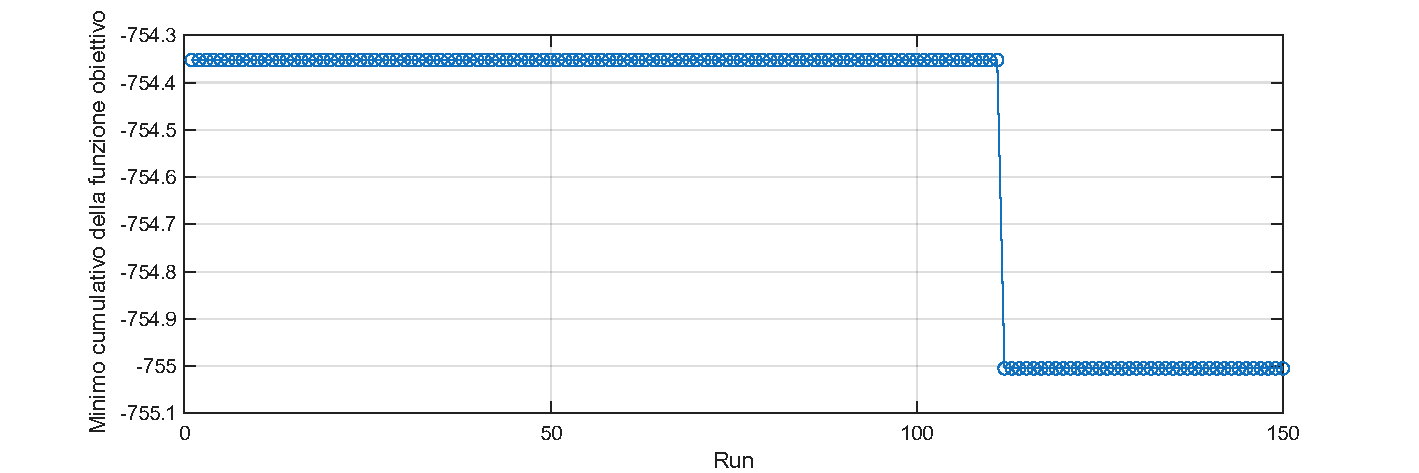
\includegraphics[width=1.1\linewidth]
    {Graphics/turbogetto/prestazioni/minimo_comulativo2.pdf}
    \caption{Andamento del minimo cumulativo della funzione obiettivo
    nelle 150 esecuzioni indipendenti dell'ottimizzazione del turbogetto.}
    \label{app:fig:cumulative_min_turbojet}
\end{figure}

\begin{figure}[H]
    \centering
    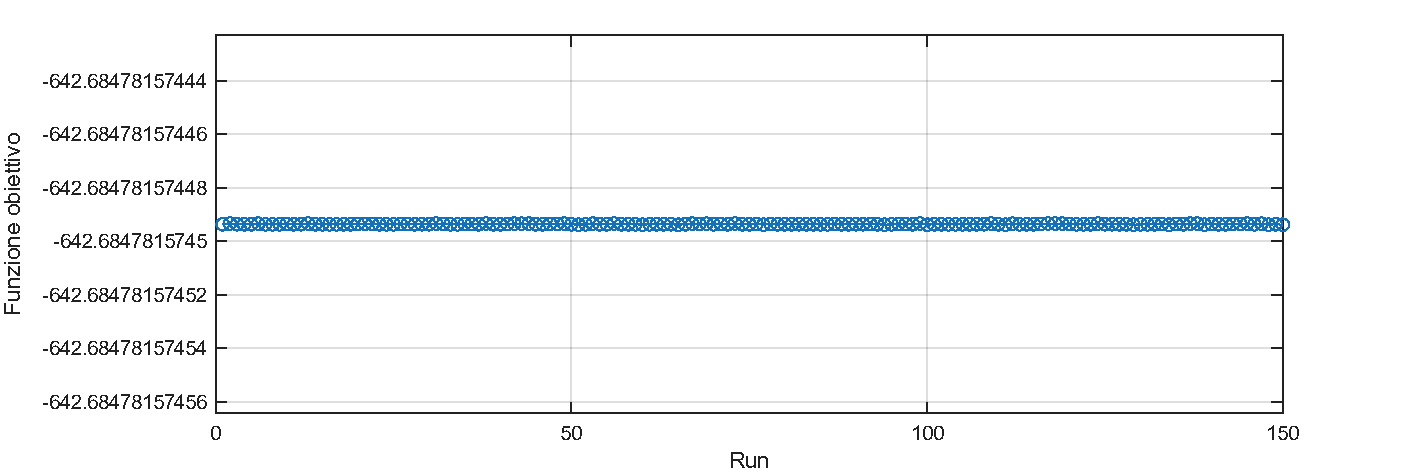
\includegraphics[width=1.1\linewidth]
    {Graphics/turbogetto/prestazioni/minimo_comulativo_ramjet}
    \caption{Andamento del minimo cumulativo della funzione obiettivo
    nelle 150 esecuzioni indipendenti dell'ottimizzazione del ramjet.}
    \label{app:fig:cumulative_min_ramjet}
\end{figure}

In entrambi i casi, la progressiva stabilizzazione del minimo cumulativo
mostra che l'aumento del numero di esecuzioni non determina ulteriori
riduzioni significative della funzione obiettivo. Tale comportamento
fornisce un'indicazione della limitata dipendenza delle soluzioni finali
dalle popolazioni iniziali.


%------------------------------------------
\section{Calcolo condizioni di volo turbogetto}
\label{app:appendiceA.1}
Le grandezze termodinamiche alla quota di volo $h=12000$ m possono essere calcolate utilizzando il modello dell'Atmosfera Standard Internazionale (ISA) dal quale si ricavano le seguenti grandezze statiche \cite{USStandardAtmosphere1976}.

\begin{align*}
    P_s = 19330 \, \text{Pa}\\
    T_s = 216.7 \,\text{K}
\end{align*}

Considerando un numero di Mach pari a $M =0.85$ imposto dalla missione, la velocità di volo risulta:

\begin{gather*}
    a = \sqrt{\gamma R T_s} = 295.1 \,\text{m/s}\\
    v_{\text{volo,tj}} = aM = 250.8 \,\text{m/s}
\end{gather*}

Calcolo delle grandezze totali
\begin{align*}
    T_{0}  &= T_s \left( 1 + \frac{\gamma-1}{2}M^2\right) = 248.0K \\
    P_{0}   &= P_s\left( 1 + \frac{\gamma-1}{2}M^2\right)^{\frac{\gamma}{\gamma-1}} = 30920Pa 
\end{align*}

\section{Calcolo delle condizioni di volo del ramjet}
Le grandezze termodinamiche alla quota di volo $h = 25000$ m vengono calcolate mediante il modello ISA:

\begin{gather*}
    P_s = 2549 \, \text{Pa}\\
    T_s = 221.7 \,\text{K}
\end{gather*}

Imponendo il numero di Mach di missione pari a $M = 3.5$ la velocità di volo risulta:

\begin{gather}
    a = \sqrt{\gamma R T_s} = 298.5 \,\text{m/s} \notag\\
    v_{\text{volo,rj}} = aM = 1045 \,\text{m/s}
    \label{eq:AppAVelocitàVoloRamjet}
\end{gather}

Le grandezze totali risultano:

\begin{align*}
    T_{0} &= T_s \left( 1 + \frac{\gamma-1}{2}M^2\right)
           = 765 \,\text{K} \\
    P_{0} &= P_s \left( 1 + \frac{\gamma-1}{2}M^2\right)^{\frac{\gamma}{\gamma-1}}
           = 194 \,\text{KPa}
\end{align*}

\section{Vincoli di volo ramjet}

La missione prevede una spinta totale di 65 kN. Il ramjet deve consumare al massimo $48000$ kg di carburante nella configurazione a due motori per coprire un range di $5000$ km alla velocità di volo calcolata \eqref{eq:AppAVelocitàVoloRamjet}. Pertanto un singolo motore deve consumare al massimo $m_{\text{c,disp}}$ = $24000$ kg di carburante.
Il tempo di missione può essere calcolato come

\begin{equation*}
    t_{\text{missione}} =
    \frac{\text{Range}}{v_{\text{volo,rj}}}
    = 4785 \,\text{s}
\end{equation*}

È quindi possibile calcolare la portata massima di carburante per completare la missione:

\begin{equation*}
    \dot{m}_{\text{c,max}} =
    \frac{m_{\text{c,disp}}}{t_{\text{missione}}}
    = 5.016 \,\text{kg/s}
\end{equation*}

Nota la spinta richiesta per il singolo motore, è possibile calcolare il TSFC massimo. 

\begin{equation*}
    TSFC_\text{max} =
    \frac{\dot{m}_{\text{c,max}} \cdot 3600}{F}
    = 0.2778 \,\text{kg/(Nh)}
\end{equation*}

\section{Spillamento d'aria per il raffreddamento della turbina}
\label{app:sezione:spillamentoArea}

Il raffreddamento della turbina è necessario per consentire il funzionamento ad alte temperature del motore. La portata d'aria richiesta può essere stimata a partire dalla temperatura SOT (Stator Outlet Temperature), calcolata in condizioni di blocco sonico del NGV (Nozzle Guide Vane) mediante la relazione \cite{slidesRobertoAndriani}:
\begin{equation}
    SOT = \frac{2}{\gamma_g+1}T_{04}
    \label{appA:eq:SOT}
\end{equation}

I dati di \cite{slidesRobertoAndriani} e la valutazione della $SOT$ tramite la Eq. \ref{appA:eq:SOT} permettono di determinare la frazione di aria spillata in funzione della temperatura di uscita dalla camera di combustione $T_{04}$, come mostrato in Figura \ref{appA:fig:frazioneDiAriaSpillata}.

\begin{figure} [H]
    \centering
    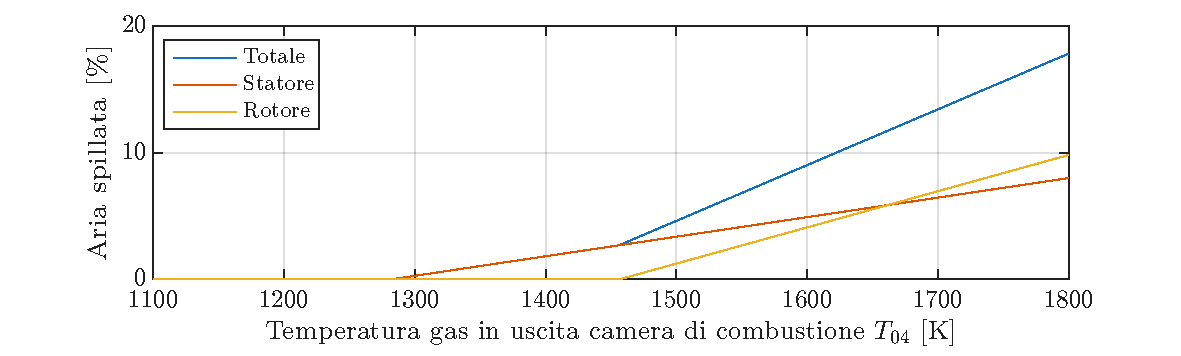
\includegraphics[width=0.9\linewidth]{Graphics/turbogetto/turbina/coolPercentagevsT04.pdf}
    \caption{Frazione di aria spillata dal compressore (\%) in funzione della temperatura $T_{04}$ [K].}
    \label{appA:fig:frazioneDiAriaSpillata}
\end{figure}

Posto il limite di $SOT \in [1100,1650] \text{ K}$, le funzioni analitiche per statore, rotore e totale che descrivono l'aria spillata dal compressore presentano la seguente formulazione in funzione della variabile di calcolo $SOT$:

\begin{equation*}
x_{\text{spillata, statore}}(\text{SOT}) = \begin{cases} 
0 & \text{se } \text{SOT} < 1100 \text{ K} \\ 
\frac{0.09}{550}(\text{SOT} - 1100) & \text{se } 1100 \le \text{SOT} \le 1650 \text{ K} 
\end{cases}
\end{equation*}

\begin{equation*}
x_{\text{spillata, rotore}}(\text{SOT}) = \begin{cases} 
0 & \text{se } \text{SOT} < 1250 \text{ K} \\ 
\frac{0.05}{350}(\text{SOT} - 1250) & \text{se } 1250 \le \text{SOT} \le 1650 \text{ K} \end{cases}
\end{equation*}

aria spillata totale dal compressore:
\begin{equation*}
x_{\text{spillata}}(\text{SOT}) = \begin{cases} 
0 & \text{se } \text{SOT} < 1100 \text{ K} \\ 
\frac{0.09}{550}(\text{SOT} - 1100) & \text{se } 1100 \le \text{SOT} < 1250 \text{ K} \\ 
\frac{0.09}{550}(\text{SOT} - 1100) + \frac{0.05}{350}(\text{SOT} - 1250) & \text{se } 1250 \le \text{SOT} \le 1650 \text{ K} \\ 
\end{cases}
\end{equation*}

\chapter{Appendix B}
\label{ap:appendixB}
%------------------------------------------------------------
\section{Diffusore subsonico}
%------------------------------------------------------------
\label{app:presa_aria_subsonica}

Le condizioni di volo alla quota di progetto sono ricavate mediante il modello ISA e le relazioni riportate in Appendice~\ref{app:appendiceA.1}.

Nel modello viene considerata una presa d'aria non ideale. Il rendimento isentropico del diffusore viene imposto pari a

\begin{equation*}
\eta_d=0.975
\end{equation*}

Il corrispondente coefficiente di recupero della pressione totale è calcolato mediante la relazione 

\begin{equation*}
\pi_D=
\left(
\frac{
1+\eta_d\frac{\gamma_a-1}{2}M_0^2
}{
1+\frac{\gamma_a-1}{2}M_0^2
}
\right)^{\frac{\gamma_a}{\gamma_a-1}}
=0.989
\end{equation*}

Per l'ipotesi adiabatica la temperatura totale si conserva, mentre la perdita di pressione totale è introdotta mediante $\pi_D$:
\begin{equation*}
    T_{02}=T_{00}
\end{equation*}
\begin{equation*}
    P_{02}=\pi_D P_{00}
\end{equation*}

dove $T_{00}$ e $P_{00}$ sono le grandezze totali della corrente indisturbata, calcolate in Appendice~\ref{app:appendiceA.1}.


\subsection{Condizioni statiche all'uscita della presa d'aria}

All'uscita del diffusore è imposto un numero di Mach $M_2=0.5$. Le corrispondenti grandezze statiche sono determinate dalle relazioni isoentropiche:

\begin{equation*}
    T_2=
    \frac{T_{02}}
    {1+\frac{\gamma_a-1}{2}M_2^2}
\end{equation*}

\begin{equation*}
    P_2=
    \frac{P_{02}}
    {\left(1+\frac{\gamma_a-1}{2}M_2^2\right)^{\frac{\gamma_a}{\gamma_a-1}}}
\end{equation*}

La densità, la velocità del suono e la velocità del flusso risultano:

\begin{equation*}
    \rho_2=\frac{P_2}{R_aT_2}
\end{equation*}

\begin{equation*}
    a_2=\sqrt{\gamma_aR_aT_2}
\end{equation*}

\begin{equation*}
    V_2=M_2a_2
\end{equation*}


\subsection{Dimensionamento geometrico }

La sezione di ingresso della presa d'aria è determinata mediante l'equazione di continuità:

\begin{equation*}
A_0=
\frac{\dot{m}_{air}}
{\rho_0V_0}
\end{equation*}

La sezione all'uscita del diffusore, coincidente con la sezione di ingresso del compressore, risulta:

\begin{equation*}
A_2=
\frac{\dot{m}_{air}}
{\rho_2V_2}
\end{equation*}

Assumendo una sezione circolare, i diametri delle sezioni di ingresso e di uscita sono:

\begin{equation*}
D_1=
\sqrt{\frac{4A_0}{\pi}}
\end{equation*}

\begin{equation*}
D_2=
\sqrt{\frac{4A_2}{\pi}}
\end{equation*}

Dal rapporto tra le due sezioni si ricava:

\begin{equation*}
\frac{D_2}{D_1}
=
\sqrt{\frac{A_2}{A_0}}
\end{equation*}

Al fine di contenere la lunghezza del diffusore è stato adottato un rapporto geometrico costante pari a

\begin{equation*}
\frac{L}{D_1}=1.5.
\end{equation*}

L'angolo totale di divergenza viene quindi ricavato imponendo la geometria di un diffusore conico:

\begin{equation*}
\frac{D_2}{D_1}
=
1+
2\left(\frac{L}{D_1}\right)\tan\phi
\end{equation*}

da cui si ottiene l'angolo totale di divergenza:

\[
2\phi = 6.69^\circ.
\]

La configurazione individuata viene infine verificata mediante il diagramma riportato in Figura~\ref{fig:diffusoreSubsonico}. Il punto ottenuto ricade nella regione \emph{No appreciable stall}.

\begin{figure}[H]
    \centering
    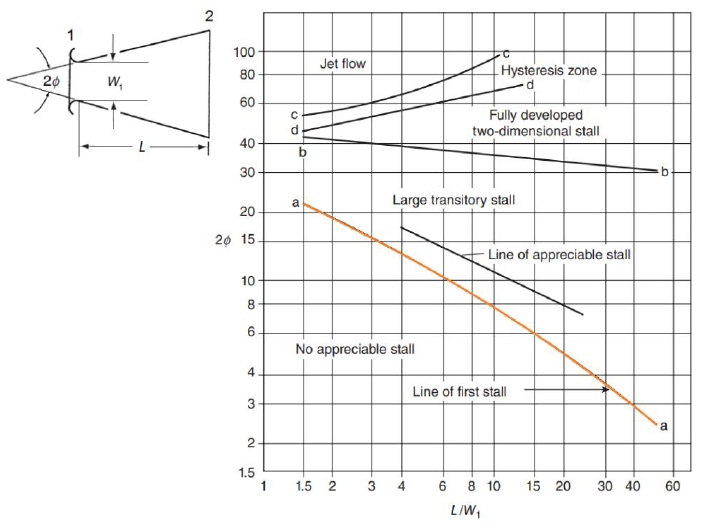
\includegraphics[width=0.82\linewidth]{Graphics/turbogetto/presaAria/Geometria_diffusore_subsonico.png}
    \caption{Diagramma utilizzato per la verifica della geometria del diffusore subsonico.}
    \label{fig:diffusoreSubsonico}
\end{figure}

La lunghezza del diffusore risulta infine:

\begin{equation*}
L=
\left(\frac{L}{D_1}\right)D_1.
\end{equation*}



%------------------------------------------------------------
\section{Compressore}
%------------------------------------------------------------
\label{app:compressore}
Il dimensionamento del compressore è stato effettuato a partire dalle
condizioni totali fornite dalla presa d'aria e dai parametri di progetto
$\pi_c$, $U_{tip}$ e $\eta_{p,c}$.

\subsection{Prestazioni termodinamiche}

Assumendo un rendimento politropico costante
$\eta_{p,c}=0.90$, il corrispondente rendimento isoentropico è

\begin{equation*}
\eta_c=
\frac{\pi_c^{\frac{\gamma_a-1}{\gamma_a}}-1}
{\pi_c^{\frac{\gamma_a-1}{\gamma_a\eta_{p,c}}}-1}.
\end{equation*}

Le condizioni totali all'uscita del compressore risultano

\begin{equation*}
P_{03}=\pi_c P_{02},
\end{equation*}

\begin{equation*}
T_{03s}=T_{02}\pi_c^{\frac{\gamma_a-1}{\gamma_a}},
\qquad
T_{03}=T_{02}+\frac{T_{03s}-T_{02}}{\eta_c}.
\end{equation*}

Il lavoro specifico e la potenza assorbita sono quindi

\begin{equation*}
l_c=c_{p,a}(T_{03}-T_{02}),
\qquad
\dot{L}_c=\dot{m}_{air}l_c.
\end{equation*}


\subsection{Dimensionamento Geometrico}

All'ingresso del compressore è imposto $M_2=0.5$. Le condizioni statiche
sono ricavate dalle corrispondenti grandezze totali:

\begin{equation*}
T_2=
\frac{T_{02}}
{1+\frac{\gamma_a-1}{2}M_2^2},
\qquad
P_2=
\frac{P_{02}}
{\left(1+\frac{\gamma_a-1}{2}M_2^2\right)^
{\frac{\gamma_a}{\gamma_a-1}}},
\end{equation*}

\begin{equation*}
\rho_2=\frac{P_2}{R_aT_2},
\qquad
a_2=\sqrt{\gamma_aR_aT_2},
\qquad
V_a=M_2a_2.
\end{equation*}

L'area anulare di ingresso è determinata dalla continuità:

\begin{equation*}
A_2=\frac{\dot{m}_{air}}{\rho_2V_a}.
\end{equation*}

Assumendo un rapporto mozzo-punta

\begin{equation*}
\lambda=\frac{r_{h,2}}{r_{t,2}}=0.5,
\end{equation*}

si ottengono

\begin{equation*}
r_{t,2}=
\sqrt{\frac{A_2}{\pi(1-\lambda^2)}},
\qquad
r_{h,2}=\lambda r_{t,2},
\end{equation*}

\begin{equation*}
r_{m,2}=\frac{r_{t,2}+r_{h,2}}{2},
\qquad
h_2=r_{t,2}-r_{h,2}.
\end{equation*}

Nota la velocità periferica di punta $U_{tip}$, ottenuta dal processo di
ottimizzazione,

\begin{equation*}
\omega=\frac{U_{tip}}{r_{t,2}},
\qquad
U=\omega r_{m,2}.
\end{equation*}

Assumendo velocità assiale e raggio di punta costanti lungo il
compressore, le condizioni statiche all'uscita sono

\begin{equation*}
T_3=T_{03}-\frac{V_a^2}{2c_{p,a}},
\qquad
a_3=\sqrt{\gamma_aR_aT_3},
\qquad
M_3=\frac{V_a}{a_3},
\end{equation*}

\begin{equation*}
P_3=
\frac{P_{03}}
{\left(1+\frac{\gamma_a-1}{2}M_3^2\right)^
{\frac{\gamma_a}{\gamma_a-1}}},
\qquad
\rho_3=\frac{P_3}{R_aT_3}.
\end{equation*}

La geometria della sezione di uscita è quindi determinata mediante

\begin{equation*}
A_3=\frac{\dot{m}_{air}}{\rho_3V_a},
\qquad
r_{t,3}=r_{t,2},
\end{equation*}

\begin{equation*}
r_{h,3}=
\sqrt{r_{t,3}^2-\frac{A_3}{\pi}},
\qquad
r_{m,3}=\frac{r_{t,3}+r_{h,3}}{2},
\qquad
h_3=r_{t,3}-r_{h,3}.
\end{equation*}


\subsection{Dimensionamento del primo stadio}

Il primo stadio è dimensionato al raggio medio assumendo velocità assiale
costante e ingresso assiale nel rotore:

\begin{equation*}
V_{\theta,1}=0,
\qquad
W_{\theta,1}=V_{\theta,1}-U,
\qquad
W_1=\sqrt{V_a^2+W_{\theta,1}^2}.
\end{equation*}

Per il dimensionamento preliminare viene imposto il limite di De Haller

\begin{equation*}
\frac{W_2}{W_1}=0.72,
\end{equation*}

da cui

\begin{equation*}
W_2=0.72W_1,
\qquad
W_{\theta,2}=-\sqrt{W_2^2-V_a^2},
\qquad
V_{\theta,2}=W_{\theta,2}+U.
\end{equation*}

Applicando l'equazione di Eulero, il lavoro specifico teorico dello
stadio risulta

\begin{equation*}
l_{st,teo}=U(V_{\theta,2}-V_{\theta,1}),
\end{equation*}

da cui viene stimato il numero di stadi:

\begin{equation*}
N_{stadi}
=
\left\lceil
\frac{l_c}{l_{st,teo}}
\right\rceil.
\end{equation*}

Poiché $N_{stadi}$ deve assumere un valore intero, il lavoro specifico
viene successivamente ridistribuito uniformemente tra gli stadi:

\begin{equation*}
l_{st}=\frac{l_c}{N_{stadi}},
\end{equation*}

e il triangolo di velocità viene ricalcolato mediante

\begin{equation*}
V_{\theta,2}
=
V_{\theta,1}+\frac{l_{st}}{U}.
\end{equation*}

Le velocità risultanti sono quindi

\begin{align*}
V_1 &= \sqrt{V_a^2+V_{\theta,1}^2}, &
V_2 &= \sqrt{V_a^2+V_{\theta,2}^2},\\
W_{\theta,1} &= V_{\theta,1}-U, &
W_{\theta,2} &= V_{\theta,2}-U,\\
W_1 &= \sqrt{V_a^2+W_{\theta,1}^2}, &
W_2 &= \sqrt{V_a^2+W_{\theta,2}^2}.
\end{align*}

Il fattore di De Haller finale viene pertanto verificato sul triangolo
ricalcolato e può risultare superiore al valore limite inizialmente
imposto.


\subsection{Verifiche aerodinamiche}

Sul triangolo di velocità ricalcolato vengono valutati

\begin{equation*}
DeHaller=\frac{W_2}{W_1},
\qquad
C_p=1-\left(\frac{W_2}{W_1}\right)^2,
\end{equation*}

e gli angoli relativi del rotore

\begin{equation*}
\beta_1=\arctan\left(\frac{W_{\theta,1}}{V_a}\right),
\qquad
\beta_2=\arctan\left(\frac{W_{\theta,2}}{V_a}\right).
\end{equation*}

I massimi numeri di Mach assoluto e relativo sono

\begin{equation*}
M_{abs}=
\max\left(\frac{V_1}{a_2},\frac{V_2}{a_2}\right),
\qquad
M_{rel}=
\max\left(\frac{W_1}{a_2},\frac{W_2}{a_2}\right).
\end{equation*}

Assumendo $\sigma_r=1.0$ e $\sigma_s=1.25$, i coefficienti di
diffusione di rotore e statore sono

\begin{equation*}
D_r=
1-\frac{W_2}{W_1}
+
\frac{|V_{\theta,2}-V_{\theta,1}|}
{2\sigma_r W_1},
\end{equation*}

\begin{equation*}
D_s=
1-\frac{V_a}{V_2}
+
\frac{|V_{\theta,2}-V_{\theta,1}|}
{2\sigma_s V_2}.
\end{equation*}

Il grado di reazione al raggio medio è

\begin{equation*}
R=
1-\frac{V_{\theta,1}+V_{\theta,2}}{2U}.
\end{equation*}


\subsection{Numero di pale rotoriche}

La corda al raggio medio viene determinata imponendo

\begin{equation*}
Re_c=\frac{W_1c_m}{\nu}\geq 3\times10^5.
\end{equation*}

Assumendo il valore limite,

\begin{equation*}
c_m=\frac{3\times10^5\,\nu}{W_1}.
\end{equation*}

Dalla solidity rotorica $\sigma_r=c_m/s_r=1$ segue

\begin{equation*}
s_r=\frac{c_m}{\sigma_r},
\end{equation*}

e il numero di pale viene determinato come

\begin{equation*}
N_{pale,r}
=
\left\lceil
\frac{2\pi r_{m,2}}{s_r}
\right\rceil.
\end{equation*}


\section{Diffusore}
\label{app:diffusore}

Si riporta di seguito la catena di calcolo completa alla base dei risultati del diffusore di raccordo compressore-camera, presentati nella Sezione~\ref{sec:camera}.

Le condizioni di ingresso ($T_{03}$, $P_{03}$, $M_3$) coincidono con le grandezze totali e il numero di Mach in uscita dal compressore. La temperatura totale si conserva lungo il condotto (trasformazione adiabatica), mentre la pressione totale è ridotta dal rendimento pneumatico assegnato:
\begin{equation*}
    T_{03.5} = T_{03}, \qquad P_{03.5} = \pi_d\,P_{03}.
\end{equation*}

Le grandezze statiche in ingresso, necessarie per il calcolo dell'area di passaggio, si ottengono dalle relazioni isoentropiche applicate al Mach $M_3$:
\begin{equation*}
    T_3 = \frac{T_{03}}{1+\dfrac{\gamma-1}{2}M_3^2}, \qquad
    P_3 = \frac{P_{03}}{\left(1+\dfrac{\gamma-1}{2}M_3^2\right)^{\gamma/(\gamma-1)}}, \qquad
    \rho_3 = \frac{P_3}{R\,T_3},
\end{equation*}
da cui la velocità $v_3 = M_3\sqrt{\gamma R T_3}$ e, per continuità, la sezione di ingresso:
\begin{equation*}
    A_3 = \frac{\dot{m}_{aria}}{\rho_3\,v_3}.
\end{equation*}

Le medesime relazioni, valutate sul Mach di uscita imposto $M_{3.5}$ e sulle grandezze totali $T_{03.5}$, $P_{03.5}$, forniscono le condizioni statiche e la sezione di uscita:
\begin{equation*}
    T_{3.5} = \frac{T_{03.5}}{1+\dfrac{\gamma-1}{2}M_{3.5}^2}, \qquad
    P_{3.5} = \frac{P_{03.5}}{\left(1+\dfrac{\gamma-1}{2}M_{3.5}^2\right)^{\gamma/(\gamma-1)}}, \qquad
    \rho_{3.5} = \frac{P_{3.5}}{R\,T_{3.5}},
\end{equation*}
\begin{equation*}
    v_{3.5} = M_{3.5}\sqrt{\gamma R T_{3.5}}, \qquad A_{3.5} = \frac{\dot{m}_{aria}}{\rho_{3.5}\,v_{3.5}}.
\end{equation*}

Assumendo una geometria anulare con raggio medio $r_{medio}$ coincidente con quello dell'ultimo stadio del compressore, le altezze del canale in ingresso e in uscita si ricavano da
\begin{equation*}
    h_3 = \frac{A_3}{2\pi\,r_{medio}}, \qquad h_{3.5} = \frac{A_{3.5}}{2\pi\,r_{medio}}.
\end{equation*}

La lunghezza assiale del diffusore è infine determinata imponendo il semi-angolo di apertura $\theta$, in modo da limitare il rischio di distacco dello strato limite lungo le pareti divergenti:
\begin{equation*}
    L_D = \frac{h_{3.5}-h_3}{2\tan\theta}.
\end{equation*}

%------------------------------------------------------------
\section{Camera di Combustione}
%------------------------------------------------------------
\label{app:camera_combustione}


Si riporta di seguito la catena di calcolo completa alla base dei risultati presentati nella Sezione~\ref{sec:camera}, relativa al modello a doppia zona del combustore anulare nel punto di progetto turbogetto.

\subsection{Grandezze statiche in ingresso}

Le condizioni disponibili a valle del diffusore ($P_{03}'$, $T_{03}'$, $M_{03}'$) sono espresse in termini di grandezze totali. Il calcolo della densità del flusso in ingresso alla camera richiede le corrispondenti grandezze statiche, ottenute mediante le relazioni isoentropiche:
\begin{equation*}
    T_3 = \frac{T_{03}'}{1 + \dfrac{\gamma_a - 1}{2} M_{03}'^2}, \qquad
    P_3 = \frac{P_{03}'}{\left(1 + \dfrac{\gamma_a - 1}{2} M_{03}'^2\right)^{\gamma_a/(\gamma_a - 1)}}, \qquad
    \rho_3 = \frac{P_3}{R_a T_3}.
\end{equation*}

\subsection{Rapporti combustibile/aria e rapporto di equivalenza}

Applicando il bilancio entalpico separatamente nella zona primaria (a temperatura $T_{comb}$) e sull'intero sistema (a temperatura $T_{04}$) si ottengono rispettivamente il rapporto combustibile/aria locale e quello globale:
\begin{equation*}
    f_{liner} = \frac{c_{p,g}\,T_{comb} - c_{p,a}\,T_{03}'}{LHV\,\eta_b - c_{p,g}\,T_{comb} + c_{p,f}\,T_{fuel}}, \qquad
    f_{global} = \frac{c_{p,g}\,T_{04} - c_{p,a}\,T_{03}'}{LHV\,\eta_b - c_{p,g}\,T_{04} + c_{p,f}\,T_{fuel}},
\end{equation*}
con $T_{fuel} = 273.15$ K temperatura di ingresso del combustibile. Il rapporto di equivalenza della zona primaria segue come
\begin{equation*}
    \phi = \frac{f_{liner}}{f_{st}}, \qquad f_{st} = 0.068.
\end{equation*}

\subsection{Suddivisione delle portate d'aria}

La frazione di portata che alimenta la zona primaria si ricava imponendo la conservazione dell'entalpia nella miscelazione adiabatica tra i gas a $T_{comb}$ e l'aria fredda by-passata a $T_{03}'$:
\begin{equation*}
    \dot{m}_{air,calda}\left(c_{p,g}T_{comb} - c_{p,a}T_{03}'\right) = \dot{m}_{air}\left(c_{p,g}T_{04} - c_{p,a}T_{03}'\right)
    \ \Longrightarrow \
    \dot{m}_{air,calda} = \dot{m}_{air}\,\frac{c_{p,g}T_{04} - c_{p,a}T_{03}'}{c_{p,g}T_{comb} - c_{p,a}T_{03}'},
\end{equation*}
da cui $\dot{m}_{air,fredda} = \dot{m}_{air} - \dot{m}_{air,calda}$. Portata di combustibile e calore rilasciato risultano
\begin{equation*}
    \dot{m}_{comb} = f_{global}\,\dot{m}_{air}, \qquad \dot{Q} = \dot{m}_{comb}\,LHV\,\eta_b.
\end{equation*}

\subsection{Dimensionamento trasversale}

Dalla correlazione $\Delta P/q_{ref} = \text{cost}$ si ricava la sezione di riferimento:
\begin{equation*}
    A_{ref} = \sqrt{\frac{R_g}{2}\left(\frac{\dot{m}_{air}\sqrt{T_{03}'}}{P_{03}'}\right)^2 \frac{k_{din}}{\Delta P/P_{03}'}},
\end{equation*}
con $k_{din}$ coefficiente di perdita dinamica. Dal raggio medio anulare ereditato dal compressore, $r_{medio} = r_{M3}$, si ottiene l'altezza del canale $h_{ref} = A_{ref}/(2\pi\,r_{medio})$, mentre le grandezze di verifica nella sezione di riferimento sono
\begin{equation*}
    U_{ref} = \frac{\dot{m}_{air}}{\rho_3\,A_{ref}}, \qquad q_{ref} = \frac{1}{2}\rho_3 U_{ref}^2, \qquad M_{ref} = \frac{U_{ref}}{\sqrt{\gamma_g R_g T_{03}'}}.
\end{equation*}
Per il calcolo del tempo di residenza sono necessarie le grandezze locali nel liner, ottenute scalando l'area di riferimento sulla sola frazione di portata calda:
\begin{equation*}
    A_{liner} = A_{ref}\,\frac{\dot{m}_{air,calda}}{\dot{m}_{air}}, \qquad \rho_{liner} = \frac{P_3}{R_g\,T_{comb}}, \qquad U_{liner} = \frac{\dot{m}_{air,calda} + \dot{m}_{comb}}{A_{liner}\,\rho_{liner}}.
\end{equation*}

\subsection{Dimensionamento volumetrico, longitudinale e verifica del tempo di residenza}

Dal vincolo sull'intensità di combustione $I = \dot{Q}/(V\,P_{03}')$ si ricava il volume della camera e, nota $A_{ref}$, la lunghezza assiale:
\begin{equation*}
    V = \frac{\dot{Q}}{I\,P_{03}'}, \qquad L_c = \frac{V}{A_{ref}}.
\end{equation*}
Il tempo di residenza nella zona primaria, confrontato con il vincolo $t_{res} > 8$ ms imposto in ottimizzazione, è dato da
\begin{equation*}
    t_{res} = \frac{L_c}{U_{ref}}.
\end{equation*}

\subsection{Condizioni di uscita}

Pressione e temperatura totali in uscita dalla camera risultano
\begin{equation*}
    P_{04} = \left(1 - \frac{\Delta P}{P_{03}'}\right)P_{03}', \qquad T_{04} = \text{TIT imposta in ottimizzazione (Sezione 1.2)}.
\end{equation*}

Di seguito viene schematizzata la ripartizione del flusso d'aria e le successive fasi di trasformazione termodinamica all'interno della camera di combustione:
\begin{figure}[H]
    \centering
    \resizebox{\textwidth}{!}{%
    \begin{tikzpicture}[
        node distance = 10mm and 14mm,
        box/.style = {rectangle, draw, rounded corners=2pt, minimum width=30mm, minimum height=11mm,
                       align=center, font=\small, fill=gray!8},
        arr/.style = {-{Latex[length=2mm]}, thick},
        lbl/.style = {font=\scriptsize, align=center, fill=white, inner sep=1pt}
    ]

        \node[box] (diff) {Diffusore\\(uscita)\\[1pt]\footnotesize $T_{03}'$, $P_{03}'$};

        \node[box, above right=14mm and 24mm of diff, fill=orange!12] (liner) {Zona primaria\\(liner)\\[1pt]\footnotesize $T_{comb}$};

        \node[box, below right=14mm and 24mm of diff, fill=teal!10] (dil) {Aria di\\diluizione\\[1pt]\footnotesize $T_{03}'$};

        \node[box, right=24mm of diff, fill=violet!10] (mix) at ($(liner)!0.5!(dil)+(24mm,0)$) {Miscelazione\\adiabatica};

        \node[box, right=14mm of mix, fill=gray!15] (out) {Uscita\\camera\\[1pt]\footnotesize $T_{04}$, $P_{04}$};

        \node[above=6mm of liner, font=\scriptsize] (fuel) {JP-7};

      
        \draw[arr] (diff.east) -- ++(6mm,0) |- (liner.west) node[lbl, pos=0.3, above] {$\dot{m}_{air,calda}$};
        \draw[arr] (diff.east) -- ++(6mm,0) |- (dil.west) node[lbl, pos=0.3, below] {$\dot{m}_{air,fredda}$};
        \draw[arr] (fuel) -- (liner.north) node[lbl, midway, right] {$\dot{m}_{comb}$};

    
        \draw[arr] (liner.south) -- ++(0,-5mm) -| (mix.north);
   
        \draw[arr] (dil.north) -- ++(0,5mm) -| (mix.south);

        \draw[arr] (mix.east) -- (out.west) node[lbl, midway, above] {$\dot{m}_{gas}$};

        % Portata totale in ingresso
        \node[lbl, above=1mm of diff, fill=none] {$\dot{m}_{air}$};

    \end{tikzpicture}%
    }
    \caption{Schema funzionale della camera di combustione e ripartizione delle portate massiche.}
    \label{fig:schema_camera}
\end{figure}



%------------------------------------------------------------
\section{Turbina}
%------------------------------------------------------------
\label{appB:turbina}

Il lavoro prodotto dalla turbina è calcolato applicando un rendimento al lavoro del compressore. Tale rendimento serve a tenere conto degli attriti meccanici e di tutti i sistemi che richiedono potenza generata dalla turbina (elettrico, idraulico...). Pertanto viene applicato il rendimento meccanico $\eta_m = 0.95$:
\begin{equation*}
   \dot{L}_{\text{turbina}} = \frac{\dot{L}_{\text{compressore}}}{\eta_m}
\end{equation*}

Si definisce la frazione di aria spillata dal compressore come:
\begin{equation*}
    x_{\text{spillaggio}}(T_{\text{04}}) = \frac{\dot{m}_{\text{spillata}}}{\dot{m}_{\text{totale}}} 
\end{equation*}

Tale grandezza è funzione della temperatura di combustione del turbogetto e si ricava tramite Appendice~\ref{ap:appendixA}. Notare che la $\dot{m}_\text{totale}$ corrisponde alla portata totale in uscita dal motore, mentre la percentuale ricavata in Appendice ~\ref{ap:appendixA} corrisponde alla percentuale di aria spillata dal compressore. Pertanto:
\begin{equation*}
    x_\text{spillaggio} = \frac{x_\text{spillata(SOT)}\dot{m}_\text{aria}}{\dot{m}_\text{totale}}
\end{equation*}



La portata in uscita dalla camera di combustione si esprime come:
\begin{equation*}
    \dot{m}_{\text{camera}} = (1 - x_{\text{spillaggio}}) \dot{m}_{\text{totale}} 
\end{equation*}

\textbf{Grandezze totali all'uscita della turbina}\\
Applicando la conservazione dell'energia per un sistema aperto in condizioni
stazionarie, l'equazione di bilancio si riduce a:
\begin{align*}
    \frac{dE}{dt} &= \sum_{k}\dot{m}_k h_{0,k} + \dot{Q}^{\leftarrow} - \dot{L}^{\rightarrow} = 0 \\
    &= \dot{m}_{\text{camera}} c_{p,\text{g}} T_{04} + \dot{m}_{\text{spillata}} c_{p,\text{a}} T_{03} - \dot{m}_{\text{totale}} c_{p,\text{g}} T_{05} +\dot{Q}_{\text{turbina}}- \dot{L}_{\text{turbina}}  = 0
\end{align*}
Facendo l'ipotesi di turbina adiabatica e riarrangiando l'equazione di bilancio per esplicitare la temperatura di fine espansione $T_{05}$, si ottiene:
\begin{equation*}
    T_{05} = T_{04} (1 - x_{\text{spillaggio}}) + x_{\text{spillaggio}} \frac{c_{p,\text{a}}}{c_{p,\text{g}}} T_{03} - \frac{\dot{L}_{\text{compressore}}}{\dot{m}_{\text{totale}} c_{p,\text{g}} \eta_m}
\end{equation*}

Infine, applicando la relazione di espansione isoentropica mediante il rendimento politropico pari a $\eta_{\text{p,t}}$ = 0.9, si ricava il rapporto di pressione della turbina $\beta_{\text{turbina}}$:
\begin{equation*}
\beta_{\text{turbina}} = \left( \frac{T_{05}}{T_{04}} \right)^{\frac{\gamma_g}{(\gamma_g-1)\eta_{\text{p,t}}}}
\label{eqAPP:betaTurbinaCalc}
\end{equation*}
La pressione totale all'uscita della turbina si calcola come:
\begin{equation*}
P_{05} = \beta_{\text{turbina}} P_{04}
\end{equation*}

Il rendimento isoentropico della turbina è definito come:
\begin{equation*}
    \eta_t = \frac{\dot{L}_{\text{reale}}}{\dot{L}_{\text{ideale}}} = \frac{1 - \beta^{\frac{\gamma-1}{\gamma} \eta_{\text{p,t}}}}{1 - \beta^{\frac{\gamma-1}{\gamma}}}
\end{equation*}

\subsection{Stadio della turbina}
L'analisi è focalizzata sul singolo stadio (primo stadio) i cui parametri operativi sono successivamente estesi per determinare il numero di stadi complessivi della turbina.
Nello sviluppo del modello si assumono le seguenti ipotesi semplificative:
\begin{itemize}
\item Si trascura ogni perdita di pressione nello statore e nel rotore. Di conseguenza, la componente assiale della velocità è considerata costante ($v_{z} = \text{cost}$).
\item Il raggio medio della turbina coincide con il raggio medio dell'ultimo stadio del compressore.
\item Si considera un turbogetto a singolo albero, pertanto la velocità angolare $\omega$ della turbina coincide con quella del compressore.
\end{itemize}

Per permettere di calcolare le grandezze nello stadio di una turbina raffreddata si applica una semplificazione: una miscelazione adiabatica a pressione totale costante dopo lo statore del primo stadio con tutta l'aria di raffreddamento. Tale temperatura si calcola come:
\begin{equation}
T_{0M} = \frac{(1 - x_{\text{spillaggio}}) c_{p,g} T_{04} + x_{\text{spillaggio}} c_{p,a} T_{\text{spillaggio}}}{(1 - x_{\text{spillaggio}}) c_{p,g} + x_{\text{spillaggio}} c_{p,a}}
\label{appB:turbina:eq:miscelazione}
\end{equation}
La pressione totale $P_{0M}$ rimane invariata pari a $P_{04}.$ Inoltre si è ipotizzato che per tale miscelazione le velocità non vengono influenzate. 

Per chiarezza, nella turbina le proprietà nello statore/rotore hanno la seguente nomenclatura:
\begin{itemize}
    \item $[var]_1 \,\,\,=$ proprietà all'ingresso dello statore
    \item $[var]_\text{1.5} =$ proprietà all'uscita dello statore equivalenti all'ingresso del rotore
    \item $[var]_\text{2}\,\,\,=$ proprietà all'uscita del rotore
\end{itemize}

Notare che, nella divisione tra statore e rotore (1.5) vengono usati i pedici 's' statore e 'r' rotore per differenziare l'uscita dello statore con l'entrata del rotore. 


\subsection{Dimensionamento dello statore}
Nelle turbine, lo statore è utilizzato per orientare il flusso per il corretto ingresso nel rotore e in certe configurazioni il fluido viene espanso convertendo entalpia in energia cinetica. Il numero di Mach in uscita dallo statore è imposto pari a Mach = 1. Invece, le condizioni all'ingresso dello statore sono imposte dalla camera di combustione, in particolare il numero di Mach è compreso tra $0.4$ e $0.5$.

Le proprietà statiche d'ingresso si calcolano dalle grandezze totali mediante le relazioni isoentropiche:

\begin{equation*}
T_1 = T_{04} \left( 1 + \frac{\gamma_g - 1}{2} M_1^2 \right)^{-1}
\end{equation*}
\begin{equation*}
P_1= P_{04} \left( 1 + \frac{\gamma_g - 1}{2} M_1^2 \right)^{-\frac{\gamma_g}{\gamma_g - 1}} 
\end{equation*}
\begin{equation*}
    \rho_1 = \frac{P_1}{R_g T_1} 
\end{equation*}
\begin{equation*}
    v_1 = M_1 \sqrt{\gamma_g R_g T_1} 
\end{equation*}
\begin{equation*}
    A_1 = \frac{\dot{m}_\text{totale}(1-x_\text{spillaggio})}{\rho_1 v_1}
\end{equation*}


La sezione di uscita si calcola imponendo condizioni soniche all'uscita.

\begin{equation*}
T_{1.5,s} = T_{04} \left( 1 + \frac{\gamma_g - 1}{2} \right)^{-1}
\end{equation*}
\begin{equation*}
    P_{1.5,s} = P_{04} \left( 1 + \frac{\gamma_g - 1}{2} \right)^{-\frac{\gamma_g}{\gamma_g - 1}} 
\end{equation*}
\begin{equation*}
    \rho_{1.5,s} = \frac{P_{1.5,s}}{(R_g T_{1.5,s})}   
\end{equation*}
\begin{equation*}
    v_{1.5} = \sqrt{\gamma_g R_g T_{1.5,s}}
\end{equation*}
\begin{equation*}
    A_{t} = \frac{\dot{m}_\text{totale}(1-x_\text{spillaggio})}{\rho_{1.5,s} v_{1.5}}
\end{equation*}


Data la conservazione della velocità assiale, si ricavano la velocità trasversale e il relativo angolo con l'asse assiale. Pertanto:
\begin{align*}
    &v_{\theta,1.5} = \sqrt{v_{1.5}^2-v_{z,1.5}^2} =  \sqrt{v_{1.5}^2-v_{z}^2} \\
    &\alpha_{1.5}  \,\,=\arctan\left(\frac{v_{\theta,1.5}}{v_{z,1.5}}\right)
\end{align*}

\subsection{Dimensionamento del rotore}
Per la sezione di ingresso del rotore si prende in considerazione la velocità $v_\text{z} = v_\text{z,1.5}$ dato che il rotore è in rotazione. Dato che si applica una miscelazione adiabatica per simulare il raffreddamento dopo lo statore (equazione \ref{appB:turbina:eq:miscelazione}), vengono calcolate le temperature e pressioni totali e statiche per calcolare l'area di ingresso dello statore. 
\begin{equation*}
T_{1.5,r} = T_{0M} - \frac{v_{1.5}^2}{2cp_g}
\end{equation*}
\begin{equation*}
    M_{1.5,r} = \frac{v_{1.5}}{\sqrt{\gamma_gR_gT_{1.5,r}}}
\end{equation*}
\begin{equation*}
P_{1.5,r}= P_{0M} \left( 1 + \frac{\gamma_g - 1}{2} M_{1.5,r}^2 \right)^{-\frac{\gamma_g}{\gamma_g - 1}} 
\end{equation*}
\begin{equation*}
    \rho_{1.5,r} = \frac{P_{1.5,r}}{R_g T_{1.5,r}} 
\end{equation*}
\begin{equation*}
    A_{{1.5,r}} = \frac{\dot{m}_\text{totale}}{\rho_{{1.5,r}} v_{z,1.5}}
\end{equation*}

Si ricava il raggio di punta e del mozzo:
\begin{align*}
    h_{1.5} &= \frac{A_{1.5}}{2 \pi r_m} \\[6pt]
    r_{t,1.5} &= r_m + \frac{h_{1.5}}{2} \\[6pt]
r_{h,1.5} &= r_m - \frac{h_{1.5}}{2}
\end{align*}

Le velocità relative del rotore si calcolano mediante la seguente formula:
\begin{equation}
\vec{v} = \vec{w} + \vec{U}
\label{appB:eq:turbina:velocità}
\end{equation}
In particolare si calcola $w_{1.5}$ come:
\begin{equation*}
    \begin{cases}  w_{\theta,1.5} = v_{\theta,1.5} - U \\  w_{z,1.5} = v_{z,1.5} \end{cases}
\end{equation*}
La velocità U è equivalente alla velocità delle palette al raggio medio dell'ultimo stadio del compressore. Tra il compressore 
Come già discusso nella Sezione \ref{sec:turbina}, la velocità relativa in uscita dal rotore è imposta pari a Mach 0.9. Risolvendo per la velocità relativa $w_2$ utilizzando la conservazione dell'energia nel sistema di riferimento relativo:
\begin{equation*}
    a_{1.5,r} = \sqrt{\gamma_gR_gT_{1.5,r}}
\end{equation*}
\begin{equation*}
    M_{w,1.5} = \frac{\omega_{1.5}}{a_{1.5,r}}
\end{equation*}
\begin{equation*}
    w_{2} = \sqrt{\frac{a_{\text{1.5,r}}^2 + \frac{\gamma_g - 1}{2} w_{\text{1.5}}^2}{\frac{\gamma_g - 1}{2} + \frac{1}{M_{w,2}^2}}}
\end{equation*} 

Le componenti $w_\theta$ e la velocità $v_2$ si calcolano mediante Pitagora e l'equazione \eqref{appB:eq:turbina:velocità}:
\begin{equation*}
    \omega_{\theta,2} = -\sqrt{\omega _2^2-\omega_{z,2}^2} = -\sqrt{\omega _2^2-v_{z}^2}
\end{equation*}
\begin{equation*}
    \begin{cases}  v_{\theta,2} = \omega_{\theta,2} + U \\  v_{z,2} = \omega_{z,2} \end{cases}
\end{equation*}
    
Conoscendo le velocità si calcolano le proprietà termodinamiche all'uscita del rotore utilizzando l'equivalenza tra il lavoro calcolato in termini delle turbomacchine e in senso termodinamico. Si ricava che:
\begin{equation*}
T_{02} = T_{0M} - \frac{U (v_{\theta,1.5} - v_{\theta,2})}{c_{p,g}}
\end{equation*}
La pressione totale si calcola tramite una trasformazione isoentropica e viene poi utilizzata per calcolare le grandezze statiche da cui, mediante l'equazione di continuità, si calcola la grandezza dell'area all'uscita. La velocità utilizzata nell'equazione di continuità è di nuovo la sola velocità assiale.

\begin{equation*}
T_2 = T_{02} - \frac{v_2^2}{2cp_g}
\end{equation*}
\begin{equation*}
    M_2 = \frac{v_2}{\sqrt{\gamma_gR_gT_2}}
\end{equation*}
\begin{equation*}
    P_{02} = P_{0M} \left(\frac{T_{02}}{T_{0M}}\right)^{\frac{\gamma_g}{\gamma_g-1}}
\end{equation*}
\begin{equation*}
P_2= P_{02} \left( 1 + \frac{\gamma_g - 1}{2} M_2^2 \right)^{-\frac{\gamma_g}{\gamma_g - 1}} 
\end{equation*}
\begin{equation*}
    \rho_2 = \frac{P_2}{R_g T_2} 
\end{equation*}
\begin{equation*}
    A_2 = \frac{\dot{m}_\text{totale}}{\rho_2 v_{z,2}}
\end{equation*}

Si ricava il raggio di punta e del mozzo:
\begin{align*}
    h_{2} &= \frac{A_{2}}{2 \pi r_m} \\[6pt]
    r_{t,2} &= r_m + \frac{h_{2}}{2} \\[6pt]
r_{h,2} &= r_m - \frac{h_{2}}{2}
\end{align*}

Il lavoro del singolo stadio si calcola utilizzando le velocità all'ingresso e all'uscita dello statore:
\begin{equation*}
    L_{\text{stadio}} = U \left( v_{\theta,1.5} - v_{\theta,2} \right) \dot{m}_{\text{totale}}
\end{equation*}
Da tale relazione si ricava il numero di stadi della turbina, il primo stadio è uno stadio rappresentativo degli stadi, utilizzato per stimare il numero di stadi:
\begin{equation*}
    n_{\text{stadi}} = \left\lceil \frac{L_{\text{turbina}}}{L_{\text{stadio}}} \right\rceil 
\end{equation*}
Il grado di reazione della turbina invece si calcola tramite la seguente equazione:
\begin{equation*}
R = 1 - \frac{v_{\theta,1.5} + v_{\theta,2}}{2U}
\end{equation*}


\subsection{Sezioni Turbina}
La sezione di ingresso e di uscita della turbina si calcola utilizzando l'equazione di continuità. In particolare, conoscendo la velocità assiale $v_z$, le proprietà statiche si calcolano come:
\begin{equation*}
    T_4 = T_{04} -\frac{v_z^2}{2c_{p,g}}
\end{equation*}
\begin{equation*}
    M_4 = \frac{v_z}{\sqrt{\gamma_gR_gT_4}}
\end{equation*}
\begin{equation*}
    P_4 =  P_{04} \left( 1 + \frac{\gamma_g - 1}{2} M_4^2 \right)^{-\frac{\gamma_g}{\gamma_g - 1}} 
\end{equation*}
\begin{equation*}
    \rho_4 = \frac{P_4}{R_g T_4} 
\end{equation*}
\begin{equation*}
    A_4 = \frac{\dot{m}_\text{totale}(1-x_\text{spillaggio})}{\rho_4 v_z}
\end{equation*}

Per l'uscita:
\begin{equation*}
    T_5 = T_{05} -\frac{v_z^2}{2c_{p,g}}
\end{equation*}
\begin{equation*}
    M_5 = \frac{v_z}{\sqrt{\gamma_gR_gT_5}}
\end{equation*}
\begin{equation*}
    P_5 =  P_{05} \left( 1 + \frac{\gamma_g - 1}{2} M_5^2 \right)^{-\frac{\gamma_g}{\gamma_g - 1}} 
\end{equation*}
\begin{equation*}
    \rho_5 = \frac{P_5}{R_g T_5} 
\end{equation*}
\begin{equation*}
    A_5 = \frac{\dot{m}_\text{totale}}{\rho_5 v_z}
\end{equation*}

Si ricava il raggio di punta e del mozzo:
\begin{align*}
    h_5 &= \frac{A_5}{2 \pi r_m} \\[6pt]
    r_{t,5} &= r_m + \frac{h_5}{2} \\[6pt]
r_{h,5} &= r_m - \frac{h_5}{2}
\end{align*}

\subsection{Controllo dell'angolo ottimo}
L'angolo ottimo di uscita del flusso dallo statore dipende dal numero di Mach in ingresso. In particolare, tramite la Figura \ref{appB:turbina:fig:alphaottimo}, è possibile ricavare l'angolo $\alpha$ ottimo per un numero di Mach in ingresso pari a 0,5 e in uscita pari a 1.

\begin{figure}[H]
    \centering
    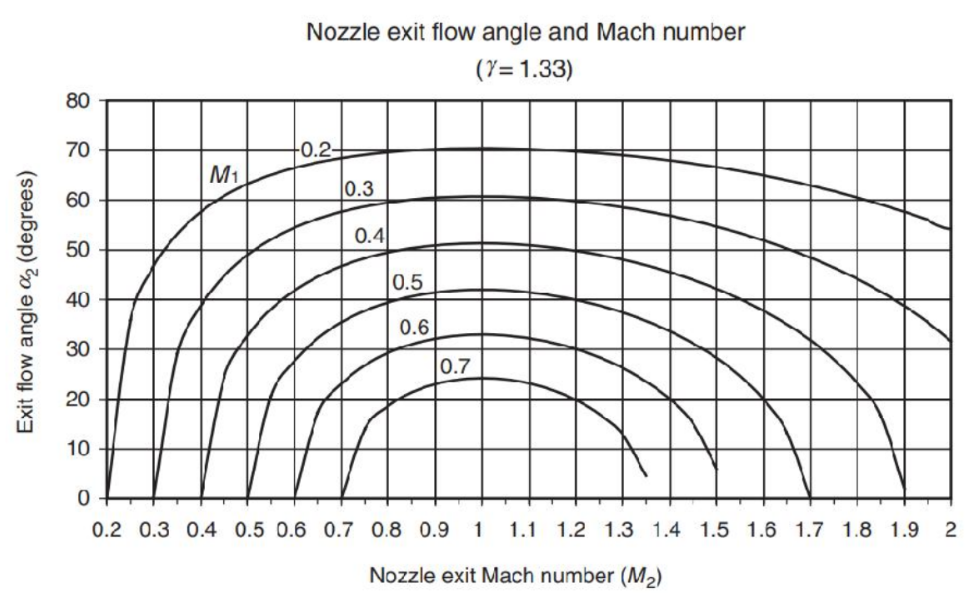
\includegraphics[width=0.7\linewidth]{Graphics/turbogetto/turbina/nozzleExit.png}
    \caption{Rappresentazione dell'angolo $\alpha$ ottimo in funzione del numero di Mach in ingresso e in uscita della turbina.}
    \label{appB:turbina:fig:alphaottimo}
\end{figure}

Per un Mach in ingresso di 0.5 l'angolo massimo risulta pari a 44°. Tale valore differisce da quello calcolato. Questa discrepanza è dovuta all'ipotesi di velocità assiale costante che impone matematicamente l'angolo a un valore di 58°. Di conseguenza la condizione di angolo $\alpha$ ottimo non risulta verificata ma in ogni caso l'angolo risulta essere prossimo alla condizione di ottimo. Una soluzione a tale problema è rimuovere il vincolo della velocità assiale costante.

\subsection{Andamento Stadio Turbina}
\begin{figure}[H]
    \centering
    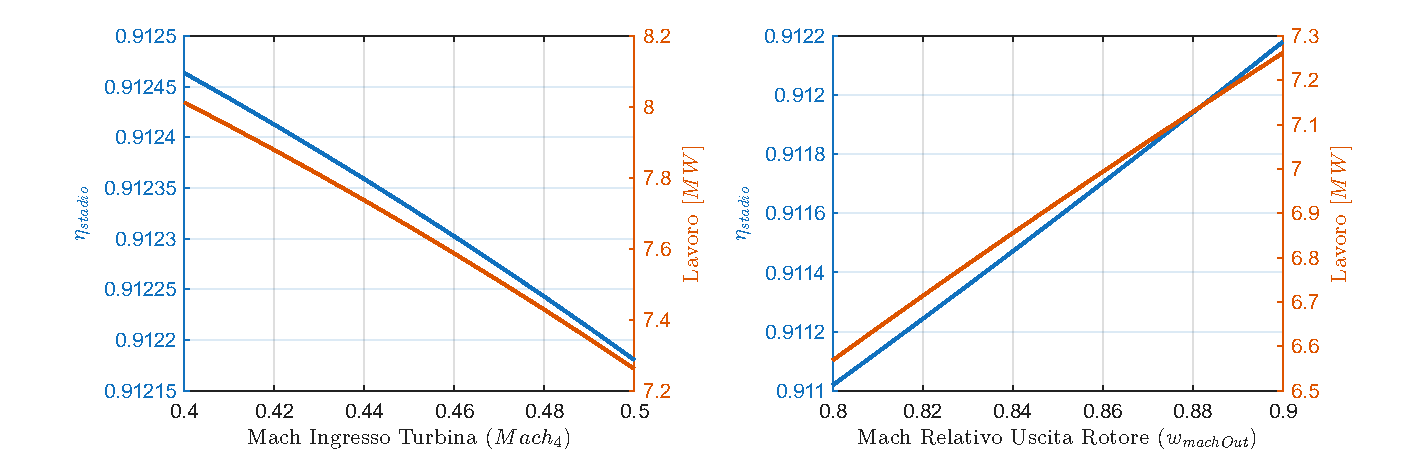
\includegraphics[width=1\linewidth]{Graphics/turbogetto/turbina/Analisi_Parametrica_Turbina__Effetto_Mach.pdf}
    \caption{(Sinistra) andamento del rendimento di stadio in funzione del numero di Mach all'ingresso della turbina.
    (Destra) andamento del rendimento di stadio in funzione del numero di Mach all'uscita del rotore.}
    \label{fig:turb:machRelativoEMachIngresso}
\end{figure}

\section{Ugello}
\label{appB:ugello}

Nel nostro caso viene considerato un ugello convergente-divergente con un rendimento \(\eta_{n}=0.95\) che opera in espansione ottima.
Nel caso il componente fosse ideale, la temperatura in uscita sarebbe:
\begin{equation*}
    T_{6_{\text{is}}} = T_{05} \text{NPR}^{\frac{1-\gamma}{\gamma}}
\end{equation*}
dove \(\text{NPR} = \frac{P_{05}}{P_{\text{amb}}}\).
Possiamo quindi ricavare il valore effettivo:
\begin{equation*}
    T_{6} = T_{05} - \eta_{n}(T_{05} - T_{06_{\text{is}}})
\end{equation*}
e trovare poi la velocità di efflusso con annesso numero di Mach:
\begin{equation*}
    u_{e} = \sqrt{2C_{p}(T_{05} - T_{6})}
\end{equation*}
\begin{equation*}
    M_{6} =\frac{u_{e}} {\sqrt{\gamma R T_{6}}}
\end{equation*}
Inoltre si ha la conservazione della temperatura totale e si ha, naturalmente, una variazione della pressione totale:
\begin{equation*}
    T_{06} =T_{05}
\end{equation*}
\begin{equation*}
    P_{06}=P_{05}(1 + \frac{\gamma-1}{2}M_{6}^2)^\frac{\gamma}{\gamma-1}
\end{equation*}
Per il dimensionamento delle aree di gola e di efflusso si fa affidamento alle seguenti formule:
\[ A^{\star}=\frac{\dot{m}\sqrt{RT_{06}}}{\Gamma P_{06}} \]
\[\frac{A_e}{A^{\star}}=\frac{1}{M_6} \left( \frac{1+\frac{\gamma-1}{2}M_6^{2}}{\frac{\gamma+1}{2}} \right)^{\frac{\gamma+1}{2(\gamma-1)}}\]


\section{Prestazioni}
\label{appB:prestazioni}
In regime subsonico le prestazioni del motore aerospaziale vengono calcolate a partire dalla velocità di volo $V_0$, dalla velocità di uscita dei gas dall'ugello $u_e$ e dalle rispettive portate di massa. I principali parametri di prestazione sono:

\textbf{Spinta} \\
\begin{equation*}
    F = \dot{m}_{\text{gas}} u_e - \dot{m}_{\text{aria}} V_0
\end{equation*}

\textbf{Consumo Specifico a Spinta (TSFC)} \\
Il consumo specifico di combustibile per unità di spinta $TSFC$ è espresso in $\left[\frac{\text{kg}}{\text{N} \cdot \text{h}}\right]$:
\begin{equation*}
    TSFC = \frac{\dot{m}_{\text{comb}}}{F} \cdot 3600
\end{equation*}

\textbf{Rendimenti del Motore} \\
I rendimenti descrivono la conversione dell'energia chimica del combustibile in potenza propulsiva:
\begin{itemize}
    \item \textbf{Rendimento Termico ($\eta_{\text{th}}$):} 
    \begin{equation*}
        \eta_{\text{th}} = \frac{\frac{1}{2} \dot{m}_{\text{gas}} u_{eq}^2 - \frac{1}{2} \dot{m}_{\text{aria}} V_0^2}{\dot{m}_{\text{comb}} LHV}
    \end{equation*}

    \item \textbf{Rendimento Propulsivo ($\eta_p$):} 
    \begin{equation*}
        \eta_p = \frac{F V_0}{\frac{1}{2} \dot{m}_{\text{gas}} u_{eq}^2 - \frac{1}{2} \dot{m}_{\text{aria}} V_0^2}
    \end{equation*}

    \item \textbf{Rendimento Globale ($\eta_g$):} 
    \begin{equation*}
        \eta_g = \eta_\text{th}\eta_p= \frac{F V_0}{\dot{m}_{\text{comb}} LHV}
    \end{equation*}
\end{itemize}

\textbf{Spinta Specifica}
\begin{equation*}
    F_s = \frac{F}{\dot{m}_{\text{aria}}}
\end{equation*}
La spinta specifica è il parametro di ottimizzazione utilizzato nel simulatore per ridurre le dimensioni del propulsore. 

\chapter{Appendix C}
\label{ap:appendixC}
\section{Presa d'Aria Supersonica}
\label{app:presa_ramjet}


\subsection{Ottimizzazione degli angoli di rampa}

La ripartizione della deflessione totale tra i tre urti obliqui è stata determinata secondo il criterio di Oswatitsch, imponendo che i tre urti abbiano la medesima componente di Mach normale $M_n$. Il problema si riduce alla ricerca di un unico parametro libero, il rapporto di pressione statica associato a $M_n$, che massimizza il recupero di pressione totale complessivo del sistema di tre urti obliqui più urto normale terminale. Tale ricerca è stata condotta numericamente mediante una funzione di ottimizzazione scalare vincolata (\texttt{fminbnd}), che esplora l'intervallo di rapporti di pressione statica ammissibili, escludendo agli estremi le soluzioni fisicamente non accettabili (onde non compressive da un lato, distacco dell'urto o flusso a valle subsonico prematuro dall'altro). Ad ogni tentativo la funzione obiettivo ricostruisce in cascata i tre urti obliqui e l'urto normale terminale a partire dal valore di $M_n$ candidato, verificando ad ogni stadio la realizzabilità fisica della soluzione (angoli reali, Mach a valle supersonico), e restituisce il recupero di pressione totale risultante. Il valore di $M_n$ che massimizza tale recupero viene poi utilizzato per la ricostruzione dettagliata dei tre urti nella fase successiva.

\subsection{Urti obliqui}

Noto $M_n$ dall'ottimizzazione, gli angoli e le grandezze a valle di ciascun urto obliquo sono calcolati in cascata, utilizzando come numero di Mach a monte di ciascun urto quello ottenuto a valle dell'urto precedente. Per il generico urto $i$-esimo, l'angolo dell'onda si ricava da
\begin{equation*}
    \theta_i = \arcsin\!\left(\frac{M_n}{M_{i-1}}\right),
\end{equation*}
mentre l'angolo di deflessione del flusso attraverso la relazione $\theta$-$\beta$-$M$:
\begin{equation*}
    \delta_i = \arctan\!\left[\frac{2\cot\theta_i\left(M_{i-1}^2\sin^2\theta_i - 1\right)}{M_{i-1}^2(\gamma+\cos 2\theta_i)+2}\right].
\end{equation*}
Il numero di Mach a valle dell'urto si ottiene dalla componente normale post-urto, comune a tutti e tre gli urti data la costanza di $M_n$,
\begin{equation*}
    M_i = \frac{1}{\sin(\theta_i-\delta_i)}\sqrt{\frac{1+\dfrac{\gamma-1}{2}M_n^2}{\gamma M_n^2 - \dfrac{\gamma-1}{2}}},
\end{equation*}
e viene utilizzato come Mach a monte per il calcolo dell'urto successivo. Il recupero di pressione totale di ciascun urto, essendo funzione della sola componente normale $M_n$ (identica per costruzione nei tre urti), risulta lo stesso per tutti e tre:
\begin{equation*}
    \pi_i = \left[\frac{\frac{\gamma+1}{2}M_n^2}{1+\frac{\gamma-1}{2}M_n^2}\right]^{\frac{\gamma}{\gamma-1}} \left[\frac{1}{\frac{2\gamma}{\gamma+1}M_n^2 - \frac{\gamma-1}{\gamma+1}}\right]^{\frac{1}{\gamma-1}}.
\end{equation*}

\subsection{Urto normale terminale}

Il terzo urto obliquo lascia il flusso ancora supersonico ($M_3>1$); la chiusura della presa avviene mediante un urto normale, per il quale il Mach a valle si ricava dalla consueta relazione delle onde d'urto normali,
\begin{equation*}
    M_4 = \sqrt{\frac{M_3^2 + \dfrac{2}{\gamma-1}}{\dfrac{2\gamma}{\gamma-1}M_3^2 - 1}},
\end{equation*}
mentre il recupero di pressione totale $\pi_4$ è dato dalla stessa espressione utilizzata per gli urti obliqui, valutata questa volta direttamente su $M_3$ (Mach a monte dell'urto normale).

\subsection{Calcolo gasdinamico a cascata}

Il recupero di pressione totale complessivo si ottiene moltiplicando i quattro contributi in cascata,
\begin{equation*}
    P_{01}=P_{00}\,\pi_1, \quad P_{02}=P_{01}\,\pi_2, \quad P_{03}=P_{02}\,\pi_3, \quad P_{04}=P_{03}\,\pi_4, \qquad \pi_{tot} = \frac{P_{04}}{P_{00}}.
\end{equation*}
L'intero processo di compressione è stato considerato adiabatico, per cui la temperatura totale si conserva dalle condizioni di volo indisturbate fino all'uscita della presa. Le condizioni statiche in ingresso alla camera di combustione (stazione 2) si ottengono dalle relazioni isoentropiche applicate al Mach subsonico $M_4$ a valle dell'urto normale:
\begin{equation*}
    T_2 = \frac{T_{00}}{1+\dfrac{\gamma-1}{2}M_4^2}, \qquad
    P_2 = \frac{P_{04}}{\left(1+\dfrac{\gamma-1}{2}M_4^2\right)^{\gamma/(\gamma-1)}}, \qquad
    \rho_2 = \frac{P_2}{R\,T_2},
\end{equation*}
da cui la velocità di ingresso in camera $V_2 = M_4\sqrt{\gamma R T_2}$. L'efficienza adiabatica della presa, che confronta il recupero di pressione totale reale con quello di una compressione isentropica alla stessa deflessione complessiva, è definita come
\begin{equation*}
    \eta_d = \frac{\pi_{tot}^{(\gamma-1)/\gamma}\left(1+\dfrac{\gamma-1}{2}M_0^2\right) - 1}{\dfrac{\gamma-1}{2}M_0^2}.
\end{equation*}

\subsection{Dimensionamento geometrico}

L'area di cattura è ricavata dalla portata d'aria richiesta dal motore, applicando la continuità alle condizioni di volo indisturbate:
\begin{equation*}
    A_{catt} = \frac{\dot{m}}{\rho_0 V_0}.
\end{equation*}
Assumendo una sezione di cattura quadrata, l'altezza e la larghezza caratteristiche risultano $h_{catt}=\sqrt{A_{catt}/2}$ e $w_{catt}=2\,h_{catt}$.

La geometria delle rampe è stata determinata imponendo la condizione di \textit{shock-on-lip}, secondo cui il labbro del cowl esterno intercetta esattamente il punto di intersezione del terzo urto obliquo. La lunghezza della prima rampa e la lunghezza della relativa onda d'urto si ricavano per via trigonometrica dal triangolo rettangolo formato dall'altezza di cattura e dall'angolo dell'onda:
\begin{equation*}
    L_{super} = \frac{h_{catt}}{\tan\theta_1}, \qquad L_{onda,1} = \frac{h_{catt}}{\sin\theta_1}.
\end{equation*}
Per la seconda e la terza rampa, le lunghezze delle rampe e delle rispettive onde d'urto si ottengono applicando il teorema dei seni al triangolo definito dall'onda incidente e dalla rampa successiva:
\begin{equation*}
    L_{rampa,12} = L_{onda,1}\,\frac{\sin(\theta_2+\delta_1-\theta_1)}{\sin(\pi-\theta_2)}, \qquad
    L_{onda,2} = L_{onda,1}\,\frac{\sin(\theta_1-\delta_1)}{\sin(\pi-\theta_2)},
\end{equation*}
\begin{equation*}
    L_{rampa,23} = L_{onda,2}\,\frac{\sin(\theta_3+\delta_2-\theta_2)}{\sin(\pi-\theta_3)}, \qquad
    L_{onda,3} = L_{onda,2}\,\frac{\sin(\theta_2-\delta_2)}{\sin(\pi-\theta_3)}.
\end{equation*}
La rampa di gola, su cui si richiude l'urto normale perpendicolarmente al flusso proveniente dal terzo urto obliquo, e l'altezza di gola si ricavano dall'ultimo triangolo caratteristico:
\begin{equation*}
    L_{rampa,34} = L_{onda,3}\cos(\theta_3-\delta_3), \qquad h_{gola} = L_{onda,3}\sin(\theta_3-\delta_3).
\end{equation*}
L'area di gola è infine ottenuta dalla continuità alle condizioni di ingresso camera,
\begin{equation*}
    A_{gola} = \frac{\dot{m}}{\rho_2 V_2}, \qquad w_{gola} = \frac{A_{gola}}{h_{gola}},
\end{equation*}
mentre $\Delta s$ il margine longitudinale del cowl rispetto allo shock-on-lip è stimato come:
\begin{equation*}
     \Delta s = 0.1\,L_{super}
\end{equation*}




\section{Anulus} 
Per il calcolo della sezione in ingresso utilizziamo la portata in entrata, essendo questa nota insieme al diametro esterno del turbogetto, quindi:
\begin{equation*}
    A_{in}=\frac{\dot{m}}{\rho u_{in}}
\end{equation*}
\begin{equation*}
    r_{in}= \sqrt{\frac{A_{in}}{\pi} + r_{ext}^2 }
\end{equation*}
Il valore del numero di Mach all'uscita è fissato a \[M=0.6\], da questo si dimensiona l'area in uscita con la quale si può ottenere questo valore
\begin{equation*}
    A_{{out}} = A_{{in}} \frac{Ma_{{in}}}{Ma_{{out}}} ( \frac{1 + \frac{\gamma-1}{2} Ma_{{out}}^2}{1 + \frac{\gamma-1}{2} Ma_{{in}}^2})^{\frac{\gamma+1}{2(\gamma-1)}}
\end{equation*}
\begin{equation*}
    r_{out}= \sqrt{\frac{A_{out}}{\pi} + r_{ext}^2 }
\end{equation*}
Per il calcolo della velocità in uscita:
\begin{equation*}
    T_{out}=\frac{T_{0_{in}}}{1+\frac{\gamma-1}{2}M_{out}^2}
\end{equation*}
\begin{equation*}
    u_{out}=M_{out}\sqrt{\gamma R T_{out}}
\end{equation*}

\section{Camera di combustione}
In seguito all'anulus si impone un'ulteriore rallentamento fino ad ottenere \[M=0.25\] noto questo possiamo calcolare l'area della camera di combustione
\begin{equation*}
    A_{{camera}} = \frac{\dot{m}_{air} \sqrt{T_{0_{in}}}}{P_{0_{in}} M_{in} \sqrt{\frac{\gamma_{aria}}{R_{aria}}}} \left( 1 + \frac{\gamma_{aria}-1}{2} M_{in}^2 \right)^{\frac{\gamma_{aria}+1}{2(\gamma_{aria}-1)}}
\end{equation*}
\begin{equation*}
    D_{camera}=2\sqrt{\frac{A_{camera}}{\pi}}
\end{equation*}
Fissato il valore del rapporto lunghezza/diametro \text{LH} e il bloccaggio \text{B} posso calcolare la lunghezza e le dimensioni dei stabilizzatori di fiamma
\begin{equation*}
    L=D_{camera}LH
\end{equation*}
\begin{equation*}
    D_{fh}=B\frac{D_{camera}}{2}
\end{equation*}
La temperatura totale si conserva mentre ho una perdita di pressione dato che $\pi_{ab}=0.96$. Ottenute queste grandezze, è possibile ricavare la portata di carburante necessaria:
\begin{equation*}
    f = \frac{c_{p,g} T_{\max} - c_{p,a} T_{0,\text{in}}}{\Delta h_{\text{fuel}} \cdot \eta_c - c_{p,g} T_{\max}},
    \label{eq:rapporto_f}
\end{equation*}
la portata di carburante può quindi essere calcolata come:
\begin{equation*}
    \dot{m}_{\text{fuel}} = f \dot{m}_{\text{air}}.
    \label{eq:portata_fuel}
\end{equation*}




\section{Ugello}
Noti i valori in ingresso (essendo gli stessi di uscita della camera di combustione) e considerato di avere una pressione in uscita pari a \[P_5=\pi_{esp}P_{amb}\] possiamo procedere in maniere analoga al caso subsonico

Nel caso il componente fosse ideale, la temperatura in uscita sarebbe:
\begin{equation*}
    T_{5_{\text{is}}} = T_{04} \text{NPR}^{\frac{1-\gamma}{\gamma}}
\end{equation*}
dove \(\text{NPR} = \frac{P_{04}}{P_{5}}\).
Considerando che la temperatura totale si conserva possiamo quindi ricavare il valore effettivo:
\begin{equation*}
    T_{5} = T_{04} - \eta_{n}(T_{05} - T_{5_{\text{is}}})
\end{equation*}
e trovare poi la velocità di efflusso con annesso numero di Mach:
\begin{equation*}
    u_{e} = \sqrt{2C_{p}(T_{04} - T_{5})}
\end{equation*}
\begin{equation*}
    M_{5} =\frac{u_{e}} {\sqrt{\gamma R T_{5}}}
\end{equation*}
Inoltre si ha, naturalmente, una variazione della pressione totale:
\begin{equation*}
    T_{05} =T_{04}
\end{equation*}
\begin{equation*}
    P_{05}=P_{04}(1 + \frac{\gamma-1}{2}M_{5}^2)^\frac{\gamma}{\gamma-1}
\end{equation*}
Per il dimensionamento delle aree di gola e di efflusso si fa affidamento alle seguenti formule:
\[ A^{\star}=\frac{\dot{m}\sqrt{RT_{05}}}{\Gamma P_{05}} \]
\[A_e=A^{\star}\frac{1}{M_5} \left( \frac{1+\frac{\gamma-1}{2}M_5^{2}}{\frac{\gamma+1}{2}} \right)^{\frac{\gamma+1}{2(\gamma-1)}}\]

\section{Prestazioni}
\label{appC:prestazioni}

In regime supersonico, a differenza del turbogetto, l'ugello del ramjet non è generalmente adattato: il vincolo geometrico imposto sul diametro di efflusso (Sezione~\ref{sec:presa_ramjet}) comporta un'espansione incompleta, con pressione statica di uscita $P_E$ diversa dalla pressione ambiente $P_U$ alla quota di crociera. Il calcolo delle prestazioni deve quindi includere, oltre al termine di quantità di moto, il contributo di spinta di pressione associato allo squilibrio tra $P_E$ e $P_U$ sulla sezione di efflusso $A_E$.

\textbf{Spinta} \\
\begin{equation*}
    F = \dot{m}_{\text{gas}}\, u_e - \dot{m}_{\text{aria}}\, V_0 + A_E\,(P_E - P_U)
\end{equation*}
dove $u_e$ è la velocità di efflusso, $V_0$ la velocità di volo e $\dot{m}_{\text{gas}}$, $\dot{m}_{\text{aria}}$ le portate massiche rispettivamente in uscita dall'ugello e in ingresso alla presa d'aria.

\textbf{Velocità di efflusso equivalente} \\
Per esprimere in forma compatta i rendimenti energetici del ciclo, il contributo di spinta di pressione viene ricondotto a un incremento della velocità di efflusso, definendo una velocità equivalente $u_{eq}$ tale che il solo termine di quantità di moto valutato con $u_{eq}$ restituisca la spinta totale:
\begin{equation*}
    u_{eq} = u_e + \frac{A_E\,(P_E - P_U)}{\dot{m}_{\text{gas}}}
\end{equation*}
Questa grandezza sostituisce $u_e$ nel calcolo dei rendimenti energetici, in modo da tenere conto correttamente anche del contributo di pressione nell'energia cinetica del getto.

\textbf{Consumo Specifico a Spinta (TSFC)} \\
Il consumo specifico di combustibile per unità di spinta $TSFC$ è espresso in $\left[\frac{\text{kg}}{\text{N}\cdot\text{h}}\right]$:
\begin{equation*}
    TSFC = \frac{\dot{m}_{\text{comb}}}{F}\cdot 3600
\end{equation*}

\textbf{Rendimenti del Motore} \\
I rendimenti descrivono la conversione dell'energia chimica del combustibile in potenza propulsiva, valutati mediante la velocità di efflusso equivalente $u_{eq}$:
\begin{itemize}
    \item \textbf{Rendimento Termico ($\eta_{\text{th}}$):}
    \begin{equation*}
        \eta_{\text{th}} = \frac{\frac{1}{2}\dot{m}_{\text{gas}}\,u_{eq}^2 - \frac{1}{2}\dot{m}_{\text{aria}}\,V_0^2}{\dot{m}_{\text{comb}}\,LHV}
    \end{equation*}
    \item \textbf{Rendimento Propulsivo ($\eta_p$):}
    \begin{equation*}
        \eta_p = \frac{F\,V_0}{\frac{1}{2}\dot{m}_{\text{gas}}\,u_{eq}^2 - \frac{1}{2}\dot{m}_{\text{aria}}\,V_0^2}
    \end{equation*}
    \item \textbf{Rendimento Globale ($\eta_g$):}
    \begin{equation*}
        \eta_g = \eta_{\text{th}}\,\eta_p = \frac{F\,V_0}{\dot{m}_{\text{comb}}\,LHV}
    \end{equation*}
\end{itemize}

\textbf{Spinta Specifica}
\begin{equation*}
    F_s = \frac{F}{\dot{m}_{\text{aria}}}
\end{equation*}
Analogamente al turbogetto, la spinta specifica costituisce il parametro di ottimizzazione utilizzato nel simulatore per contenere le dimensioni del propulsore a parità di spinta richiesta.

\chapter{Appendix D}
\label{ap:appendixD}
\section{Codice di Calcolo MATLAB}
\label{app:codici}

In questa appendice viene riportato il codice sviluppato in ambiente MATLAB per l'ottimizzazione e il dimensionamento del sistema propulsivo. Tutte le funzioni devono essere posizionate nella cartella /FunzioniMotore

\section{Script di ottimizzazione turbogetto-ramjet}
\lstinputlisting[caption={main.m}]{codice/main.m}

\section{Funzioni Motore}
Di seguito sono riportate le funzioni MATLAB necessarie per l'esecuzione dello script main.m. Per il dimensionamento del turbogetto vengono impiegate le seguenti funzioni:

\begin{itemize}
    \item structMotore.m
    \item structParametri.m
    \item runnerMotore.m 
    \item Parametri.m
    \item PresaDaria.m 
    \item Compressore.m
    \item StimaSpillaggio.m
    \item Diffusore.m
    \item CameraCombustione.m 
    \item Turbina.m
    \item Ugello.m
    \item Performance.m
\end{itemize}
Per il ramjet vengono invece utilizzate le seguenti funzioni:
\begin{itemize}
    \item structRamjet.m
    \item runnerRamjet.m 
    \item Parametri.m
    \item PresaDaria.m 
    \item Anulus.m 
    \item CameraCombustioneRamjet.m
    \item UgelloRamjet.m
    \item Performance.m
\end{itemize}

\subsection{structMotore.m}
\lstinputlisting[caption={structMotore.m}]{codice/structMotore.m}
\subsection{structParametri.m}
\lstinputlisting[caption={structParametri.m}]{codice/structParametri.m}
\subsection{runnerMotore.m}
\lstinputlisting[caption={runnerMotore.m}]{codice/runnerMotore.m}
\subsection{Parametri.m}
\lstinputlisting[caption={Parametri.m}]{codice/Parametri.m}
\subsection{PresaDaria.m}
\lstinputlisting[caption={PresaDaria.m}]{codice/PresaDaria.m}
\subsection{Compressore.m}
\lstinputlisting[caption={Compressore.m}]{codice/Compressore.m}
\subsection{StimaSpillaggio.m}
\lstinputlisting[caption={StimaSpillaggio.m}]{codice/StimaSpillaggio.m}
\subsection{Diffusore.m}
\lstinputlisting[caption={Diffusore.m}]{codice/Diffusore.m}
\subsection{CameraCombustione.m}
\lstinputlisting[caption={CameraCombustione.m}]{codice/CameraCombustione.m}
\subsection{Turbina.m}
\lstinputlisting[caption={Turbina.m}]{codice/Turbina.m}
\subsection{Ugello.m}
\lstinputlisting[caption={Ugello.m}]{codice/Ugello.m}
\subsection{Performance.m}
\lstinputlisting[caption={Performance.m}]{codice/Performance.m}
\subsection{structRamjet.m}
\lstinputlisting[caption={structRamjet.m}]{codice/structRamjet.m}
\subsection{runnerRamjet.m}
\lstinputlisting[caption={runnerRamjet.m}]{codice/runnerRamjet.m}
\subsection{Anulus.m}
\lstinputlisting[caption={Anulus.m}]{codice/Anulus.m}
\subsection{CameraCombustioneRamjet.m}
\lstinputlisting[caption={CameraCombustioneRamjet.m}]{codice/CameraCombustioneRamjet.m}
\subsection{UgelloRamjet.m}
\lstinputlisting[caption={UgelloRamjet.m}]{codice/UgelloRamjet.m}


         %% Attualmente commentata dato ci mette un sacco a caricare aggiunge 100 pagine.




% LIST OF FIGURES
\listoffigures

% LIST OF TABLES
\listoftables


% LIST OF SYMBOLS
\chapter*{List of Symbols}

\begin{longtable}{p{0.2\textwidth} p{0.55\textwidth} p{0.15\textwidth}}
    \textbf{Simbolo} & \textbf{Descrizione} & \textbf{Unità SI} \\\hline\\[-9px]
    \endfirsthead

    \multicolumn{3}{c}{{\bfseries Continua dalla pagina precedente}} \\[1ex]
    \textbf{Simbolo} & \textbf{Descrizione} & \textbf{Unità SI} \\\hline\\[-9px]
    \endhead

    \hline
    \multicolumn{3}{r}{{Continua nella pagina successiva}} \\
    \endfoot

    \hline
    \endlastfoot
    \multicolumn{3}{l}{\textbf{Simboli Latini ed Acronimi}} \\[4px]
    $A_0, A_1, A_2, \dots$ & Aree delle sezioni caratteristiche del motore & $\text{m}^2$ \\[2px]
    $A^*$ & Area di gola dell'ugello & $\text{m}^2$ \\[2px]
    $A_{\text{catt}}$ & Area di cattura della presa d'aria supersonica & $\text{m}^2$ \\[2px]
    $A_e$ & Area di efflusso dell'ugello & $\text{m}^2$ \\[2px]
    $A_{\text{ref}}$ & Sezione di riferimento della camera di combustione & $\text{m}^2$ \\[2px]
    $a$ & Velocità del suono locale & m/s \\[2px]
    $B$ & Valore di bloccaggio degli stabilizzatori di fiamma & - \\[2px]
    $C_p$ & Coefficiente di carico aerodinamico del compressore & - \\[2px]
    $c_{p,a}, c_{p,g}$ & Calore specifico a pressione costante (aria e gas combusti) & J/(kg K) \\[2px]
    $c_m$ & Corda palare al raggio medio & m \\[2px]
    $D_0, D_1, D_2$ & Diametri delle sezioni del diffusore subsonico & m \\[2px]
    $D_E, D_{\text{Eflusso}}$ & Diametro della sezione di efflusso dell'ugello & m \\[2px]
    $D_r$ & Coefficiente di diffusione aerodinamica del rotore & - \\[2px]
    $D_s$ & Coefficiente di diffusione aerodinamica dello statore & - \\[2px]
    $d$ & Diametro dello stabilizzatore di fiamma & m \\[2px]
    $De~Haller$ & Fattore di De Haller (rapporto di decelerazione) & - \\[2px]
    $F$ & Spinta propulsiva complessiva & N \\[2px]
    $F_s$ & Spinta specifica  & m/s \\[2px]
    $f$ & Rapporto combustibile/aria (Fuel-to-Air Ratio) & - \\[2px]
    $f_{\text{global}}$ & Rapporto combustibile/aria globale in camera di combustione & - \\[2px]
    $f_{\text{liner}}$ & Rapporto combustibile/aria nel liner (zona primaria) & - \\[2px]
    $f_{\text{st}}$ & Rapporto combustibile/aria stechiometrico & - \\[2px]
    $H$ & Altezza di riferimento (es. condotto stabilizzatori) & m \\[2px]
    $h$ & Quota di volo del velivolo & m \\[2px]
    $h_2, h_3, h_{1.5}, h_5$ & Altezze del canale anulare nelle relative sezioni del motore & m \\[2px]
    $h_{\text{catt}}$ & Altezza geometrica di cattura della presa d'aria & m \\[2px]
    $h_{\text{gola}}$ & Altezza della gola della presa d'aria supersonica & m \\[2px]
    $I$ & Intensità volumetrica di combustione & $\text{W}/(\text{m}^3 \text{Pa})$ \\[2px]
    $k_{\text{din}}$ & Coefficiente di perdita di pressione dinamica & - \\[2px]
    $L$ & Lunghezza del diffusore o della camera del postbruciatore & m \\[2px]
    $L_c$ & Lunghezza assiale della camera di combustione principale & m \\[2px]
    $LHV$ & Potere calorifico inferiore del combustibile (Lower Heating Value) & J/kg \\[2px]
    $L_{\text{onda},i}$ & Lunghezza dell'onda d'urto $i$-esima & m \\[2px]
    $L_{\text{rampa},ij}$ & Lunghezza della rampa supersonica tra i punti $i$ e $j$ & m \\[2px]
    $L_{\text{super}}$ & Lunghezza supersonica totale della presa d'aria a rampe & m \\[2px]
    $\dot{L}_c$ & Potenza meccanica assorbita dal compressore & W \\[2px]
    $l_c$ & Lavoro specifico di compressione & J/kg \\[2px]
    $l_{st}$ & Lavoro specifico reale scambiato per singolo stadio & J/kg \\[2px]
    $l_{st,\text{teo}}$ & Lavoro specifico teorico calcolato per singolo stadio & J/kg \\[2px]
    $M$ & Numero di Mach locale del flusso & - \\[2px]
    $M_0$ & Numero di Mach di volo indisturbato & - \\[2px]
    $M_{\text{abs}}$ & Numero di Mach assoluto massimo nelle turbomacchine & - \\[2px]
    $M_n$ & Componente normale del numero di Mach all'urto & - \\[2px]
    $M_{\text{rel}}$ & Numero di Mach relativo massimo al rotore & - \\[2px]
    $\dot{m}$ & Portata massica complessiva di aria in ingresso & kg/s \\[2px]
    $\dot{m}_{\text{air,calda}}$ & Portata massica d'aria destinata alla combustione primaria & kg/s \\[2px]
    $\dot{m}_{\text{air,fredda}}$ & Portata massica d'aria destinata alla zona di diluizione & kg/s \\[2px]
    $\dot{m}_{\text{comb}}$ & Portata massica di combustibile iniettata & kg/s \\[2px]
    $\dot{m}_{\text{gas}}$ & Portata massica dei gas combusti allo scarico & kg/s \\[2px]
    $\dot{m}_{\text{spillata}}$ & Portata in massa spillata per il raffreddamento & kg/s \\[2px]
    $\dot{m}_{\text{totale}}$ & Portata in massa in uscita dall'ugello & kg/s \\[2px]
    $N_{\text{pale},r}$ & Numero complessivo di pale rotoriche della schiera & - \\[2px]
    $N_{\text{stadi},c}, n_{\text{stadi}}$ & Numero totale di stadi del compressore o della turbina & - \\[2px]
    $NPR$ & Rapporto di pressione totale/statica dell'ugello & - \\[2px]
    $P$ & Pressione statica locale & Pa \\[2px]
    $P_{00}$ & Pressione di ristagno indisturbata del fluido & Pa \\[2px]
    $P_{01}$ & Pressione di ristagno all'ingresso della presa d'aria & Pa \\[2px]
    $P_{02}$ & Pressione di ristagno all'uscita della presa d'aria & Pa \\[2px]
    $P_{03}$ & Pressione di ristagno all'uscita del compressore & Pa \\[2px]
    $P_{04}$ & Pressione di ristagno all'uscita della camera di combustione & Pa \\[2px]
    $P_{05}$ & Pressione di ristagno all'uscita della turbina & Pa \\[2px]
    $P_{09}$ & Pressione di ristagno all'uscita dell'ugello & Pa \\[2px]
    $q_{\text{ref}}$ & Pressione dinamica valutata nella sezione di riferimento & Pa \\[2px]
    $R$ & Grado di reazione cinematico dello stadio & - \\[2px]
    $R_a, R_g$ & Costante specifica dei gas (per aria e gas combusti) & J/(kg K) \\[2px]
    $r_h$ & Raggio geometrico di mozzo (hub) & m \\[2px]
    $r_m$ & Raggio geometrico medio del canale & m \\[2px]
    $r_t$ & Raggio geometrico di punta (tip) & m \\[2px]
    $SOT$ & Temperatura totale all'uscita dello statore & K \\[2px]
    $s_r$ & Passo palare della schiera rotorica & m \\[2px]
    $T$ & Temperatura statica locale del flusso & K \\[2px]
    $T_{00}$ & Temperatura di ristagno indisturbata del fluido & K \\[2px]
    $T_{01}$ & Temperatura di ristagno all'ingresso della presa d'aria & K \\[2px]
    $T_{02}$ & Temperatura di ristagno all'uscita della presa d'aria & K \\[2px]
    $T_{03}$ & Temperatura di ristagno all'uscita del compressore & K \\[2px]
    $T_{04}$ & Temperatura di ristagno all'uscita della camera di combustione & K \\[2px]
    $T_{05}$ & Temperatura di ristagno all'uscita della turbina & K \\[2px]
    $T_{09}$ & Temperatura di ristagno all'uscita dell'ugello & K \\[2px]
    $T_{\text{comb}}$ & Temperatura raggiunta nella zona primaria di combustione & K \\[2px]
    $TSFC$ & Consumo specifico di spinta & kg/(N h) \\[2px]
    $t_{\text{res}}$ & Tempo di residenza dei gas in camera di combustione & s \\[2px]
    $U, U_{\text{tip}}$ & Velocità periferica (di trascinamento) al raggio locale o di punta & m/s \\[2px]
    $u_e, V_e$ & Velocità cinematica di efflusso dei gas dall'ugello & m/s \\[2px]
    $u_{\text{eq}}$ & Velocità di efflusso equivalente & m/s \\[2px]
    $V$ & Volume utile della camera di combustione & $\text{m}^3$ \\[2px]
    $V, v$ & Modulo della velocità assoluta del fluido & m/s \\[2px]
    $V_a, v_z$ & Componente assiale della velocità del fluido & m/s \\[2px]
    $V_\theta, v_\theta$ & Componente tangenziale della velocità assoluta & m/s \\[2px]
    $v_{\text{volo}}$ & Velocità di volo del velivolo & m/s \\[2px]
    $W, w$ & Modulo della velocità relativa del fluido (rispetto al rotore) & m/s \\[2px]
    $W_\theta, w_\theta$ & Componente tangenziale della velocità relativa & m/s \\[2px]
    $w_{\text{gola}}$ & Larghezza geometrica della gola della presa d'aria supersonica & m \\[2px]
    $x_{\text{spill}}$ & Frazione di portata d'aria spillata dal compressore in percentuale & - \\[6px]

    \multicolumn{3}{l}{\textbf{Simboli Greci}} \\[4px]
    $\alpha$ & Angolo della velocità assoluta del flusso rispetto all'asse assiale & $^\circ$ \\[2px]
    $\beta$ & Angolo della velocità relativa del flusso rispetto all'asse assiale & $^\circ$ \\[2px]
    $\gamma, \gamma_a, \gamma_g$ & Rapporto dei calori specifici a pressione e volume costante & - \\[2px]
    $\Delta P$ & Variazione o perdita di pressione attraverso un componente & Pa o \% \\[2px]
    $\Delta s$ & Margine longitudinale (offset) rispetto alla condizione di shock-on-lip & m \\[2px]
    $\delta$ & Angolo di deflessione del flusso indotto dall'onda d'urto obliqua & $^\circ$ \\[2px]
    $\delta_S$ & Spessore dello strato limite aerodinamico & m \\[2px]
    $\eta_b$ & Efficienza termochimica di combustione in camera & - \\[2px]
    $\eta_c$ & Rendimento termodinamico isoentropico del compressore & - \\[2px]
    $\eta_t$ & Rendimento termodinamico isoentropico della turbina & - \\[2px]
    $\eta_d$ & Efficienza adiabatica della presa d'aria & - \\[2px]
    $\eta_g$ & Rendimento globale dell'intero sistema propulsivo & - \\[2px]
    $\eta_m$ & Rendimento meccanico per la trasmissione di potenza all'albero & - \\[2px]
    $\eta_N, \eta_n$ & Rendimento aerodinamico di espansione dell'ugello & - \\[2px]
    $\eta_p$ & Rendimento propulsivo o di Froude del motore & - \\[2px]
    $\eta_{p,c}$ & Rendimento politropico di compressione & - \\[2px]
    $\eta_{th}$ & Rendimento termico (o termodinamico) del ciclo & - \\[2px]
    $\theta$ & Angolo di inclinazione dell'onda d'urto obliqua & $^\circ$ \\[2px]
    $\lambda$ & Rapporto geometrico mozzo-punta (hub-to-tip ratio) & - \\[2px]
    $\nu$ & Viscosità cinematica del fluido di lavoro & $\text{m}^2$/s \\[2px]
    $\pi_{ab}$ & Coefficiente di perdita di pressione totale nel postbruciatore & - \\[2px]
    $\pi_c$ & Rapporto di compressione totale del compressore & - \\[2px]
    $\pi_D$ & Coefficiente di recupero della pressione totale nel diffusore & - \\[2px]
    $\pi_{\text{esp}}$ & Fattore di sovra/sotto-espansione per l'ugello & - \\[2px]
    $\pi_{\text{tot}}$ & Recupero di pressione totale complessivo attraverso le onde d'urto & - \\[2px]
    $\rho$ & Densità o massa volumica del fluido locale & kg/$\text{m}^3$ \\[2px]
    $\sigma_r, \sigma_s$ & Solidità (solidity) della schiera palare rotorica e statorica & - \\[2px]
    $\phi$ & Rapporto di equivalenza di combustione (o angolo del diffusore) & - / $^\circ$ \\[2px]
    $\omega$ & Velocità angolare di rotazione del gruppo turbomacchine & rad/s \\[2px]
\end{longtable}



% ACKNOWLEDGEMENTS
%\chapter*{Ringraziamenti}



%\newpage
%
\chapter*{Introduction}

This document is intended to be both an example of the Polimi \LaTeX{} template for Master Theses,
as well as a short introduction to its use. It is not intended to be a general introduction to \LaTeX{} itself,
and the reader is assumed to be familiar with the basics of creating and compiling \LaTeX{} documents (see \cite{oetiker1995not, kottwitz2015latex}). 
\\
The cover page of the thesis must contain all the relevant information:
title of the thesis, name of the Study Programme and School, name of the author,
student ID number, name of the supervisor, name(s) of the co-supervisor(s) (if any), academic year.
The above information are provided by filling all the entries in the command \verb|\puttitle{}|
in the title page section of this template.
\\
Be sure to select a title that is meaningful.
It should contain important keywords to be identified by indexer.
Keep the title as concise as possible and comprehensible even to people who are not experts in your field.
The title has to be chosen at the end of your work so that it accurately captures the main subject of the manuscript. 
\\
Since a thesis might be a substantial document, it is convenient to break it into chapters.
You can create a new chapter as done in this template by simply using the following command
\begin{verbatim}
\chapter{Title of the chapter}
\end{verbatim}
followed by the body text.
\\
Especially for long manuscripts, it is recommended to give each chapter its own file.
In this case, you write your chapter in a separated \verb|chapter_n.tex| file
and then include it in the main file with the following command
\begin{verbatim}
\input{chapter_n.tex}
\end{verbatim}
It is recommended to give a label to each chapter by using the command
\begin{verbatim}
\label{ch:chapter_name}%
\end{verbatim}
where the argument is just a text string that you'll use to reference that part
as follows: \textit{Chapter~\ref{ch:chapter_one} contains \sc{an introduction to}  \dots}.\\
If necessary, an unnumbered chapter can be created by
\begin{verbatim}
\chapter*{Title of the unnumbered chapter}
\end{verbatim}

\chapter{Chapter one}
\label{ch:chapter_one}%
% The \label{...}% enables to remove the small indentation that is generated, always leave the % symbol.

In this chapter additional useful information are reported.

\section{Sections and subsections}
\label{sec:section_name}
Chapters are typically subdivided into sections and subsections, and, optionally,
subsubsections, paragraphs and subparagraphs.
All can have a title, but only sections and subsections are numbered.
A new section is created by the command
\begin{verbatim}
\section{Title of the section}
\end{verbatim}
The numbering can be turned off by using \verb|\section*{}|.
\\
A new subsection is created by the command
\begin{verbatim}
\subsection{Title of the subsection}
\end{verbatim}
and, similarly, the numbering can be turned off by adding an asterisk as follows 
\begin{verbatim}
\subsection*{}
\end{verbatim}

\section{Equations}
\label{sec:eqs}
This section gives some examples of writing mathematical equations in your thesis.

Maxwell's equations read:
\begin{subequations}
    \label{eq:maxwell}
    \begin{align}[left=\empheqlbrace]
    \nabla\cdot \bm{D} & = \rho, \label{eq:maxwell1} \\
    \nabla \times \bm{E} +  \frac{\partial \bm{B}}{\partial t} & = \bm{0}, \label{eq:maxwell2} \\
    \nabla\cdot \bm{B} & = 0, \label{eq:maxwell3} \\
    \nabla \times \bm{H} - \frac{\partial \bm{D}}{\partial t} &= \bm{J}. \label{eq:maxwell4}
    \end{align}
\end{subequations}

Equation~\eqref{eq:maxwell} is automatically labeled by \texttt{cleveref},
as well as Equation~\eqref{eq:maxwell1} and Equation~\eqref{eq:maxwell3}.
Thanks to the \verb|cleveref| package, there is no need to use \verb|\eqref|.
Remember that Equations have to be numbered only if they are referenced in the text.

Equations~\eqref{eq:maxwell_multilabels1}, \eqref{eq:maxwell_multilabels2}, \eqref{eq:maxwell_multilabels3}, and \eqref{eq:maxwell_multilabels4} show again Maxwell's equations without brace:
\begin{align}
    \nabla\cdot \bm{D} & = \rho, \label{eq:maxwell_multilabels1} \\
    \nabla \times \bm{E} +  \frac{\partial \bm{B}}{\partial t} &= \bm{0}, \label{eq:maxwell_multilabels2} \\
    \nabla\cdot \bm{B} & = 0, \label{eq:maxwell_multilabels3} \\
    \nabla \times \bm{H} - \frac{\partial \bm{D}}{\partial t} &= \bm{J} \label{eq:maxwell_multilabels4}.
\end{align}

Equation~\eqref{eq:maxwell_singlelabel} is the same as before,
but with just one label:
\begin{equation}
    \label{eq:maxwell_singlelabel}
    \left\{
    \begin{aligned}
    \nabla\cdot \bm{D} & = \rho, \\
    \nabla \times \bm{E} +  \frac{\partial \bm{B}}{\partial t} &= \bm{0},\\
    \nabla\cdot \bm{B} & = 0, \\
    \nabla \times \bm{H} - \frac{\partial \bm{D}}{\partial t} &= \bm{J}.
    \end{aligned}
    \right.
\end{equation}

\section{Figures, Tables and Algorithms}
Figures, Tables and Algorithms have to contain a Caption that describe their content, and have to be properly reffered in the text.

\subsection{Figures}
\label{subsec:figures}

For including pictures in your text you can use \texttt{TikZ} for high-quality hand-made figures,
or just include them as usual with the command
\begin{verbatim}
\includegraphics[options]{filename.xxx}
\end{verbatim}
Here xxx is the correct format, e.g. \verb|.png|, \verb|.jpg|, \verb|.eps|, \dots.

\begin{figure}[H]
    \centering
    
\includegraphics[width=0.3\textwidth]{logo_polimi_scritta.eps}
    \caption{Caption of the Figure to appear in the List of Figures.}
    \label{fig:quadtree}
\end{figure}

Thanks to the \texttt{\textbackslash subfloat} command, a single figure, such as Figure~\ref{fig:quadtree},
can contain multiple sub-figures with their own caption and label, e.g. \color{black} Figure~\ref{fig:polimi_logo1} and Figure~\ref{fig:polimi_logo2}. 

\begin{figure}[H]
    \centering
    \subfloat[One PoliMi logo.\label{fig:polimi_logo1}]{
        
\includegraphics[scale=0.5]{Images/logo_polimi_scritta.eps}
    }
    \quad
    \subfloat[Another one PoliMi logo.\label{fig:polimi_logo2}]{
        
\includegraphics[scale=0.5]{Images/logo_polimi_scritta2.eps}
    }
    \caption[Shorter caption]{This is a very long caption you don't want to appear in the List of Figures.}
    \label{fig:quadtree2}
\end{figure}


\subsection{Tables}
\label{subsec:tables}

Within the environments \texttt{table} and  \texttt{tabular} you can create very fancy tables as the one shown in Table~\ref{table:example}.
\begin{table}[H]
    \caption*{\textbf{Title of Table (optional)}}
    \centering 
    \begin{tabular}{|p{3em} c c c |}
    \hline
    \rowcolor{bluepoli!40} % comment this line to remove the color
     & \textbf{column 1} & \textbf{column 2} & \textbf{column 3} \T\B \\
    \hline \hline
    \textbf{row 1} & 1 & 2 & 3 \T\B \\
    \textbf{row 2} & $\alpha$ & $\beta$ & $\gamma$ \T\B\\
    \textbf{row 3} & alpha & beta & gamma \B\\
    \hline
    \end{tabular}
    \\[10pt]
    \caption{Caption of the Table to appear in the List of Tables.}
    \label{table:example}
\end{table}

You can also consider to highlight selected columns or rows in order to make tables more readable.
Moreover, with the use of \texttt{table*} and the option \texttt{bp} it is possible to align them at the bottom of the page. One example is presented in Table~\ref{table:exampleC}. 

\begin{table}[H]
\centering 
    \begin{tabular}{|p{3em} | c | c | c | c | c | c|}
    \hline
%    \rowcolor{bluepoli!40}
     & \textbf{column1} & \textbf{column2} & \textbf{column3} & \textbf{column4} & \textbf{column5} & \textbf{column6} \T\B \\
    \hline \hline
    \textbf{row1} & 1 & 2 & 3 & 4 & 5 & 6 \T\B\\
    \textbf{row2} & a & b & c & d & e & f \T\B\\
    \textbf{row3} & $\alpha$ & $\beta$ & $\gamma$ & $\delta$ & $\phi$ & $\omega$ \T\B\\
    \textbf{row4} & alpha & beta & gamma & delta & phi & omega \B\\
    \hline
    \end{tabular}
    \\[10pt]
    \caption{Highlighting the columns}
    \label{table:exampleC}
\end{table}

\begin{table}[H]
\centering 
    \begin{tabular}{|p{3em} c c c c c c|}
    \hline
%    \rowcolor{bluepoli!40}
     & \textbf{column1} & \textbf{column2} & \textbf{column3} & \textbf{column4} & \textbf{column5} & \textbf{column6} \T\B \\
    \hline \hline
    \textbf{row1} & 1 & 2 & 3 & 4 & 5 & 6 \T\B\\
    \hline
    \textbf{row2} & a & b & c & d & e & f \T\B\\
    \hline
    \textbf{row3} & $\alpha$ & $\beta$ & $\gamma$ & $\delta$ & $\phi$ & $\omega$ \T\B\\
    \hline
    \textbf{row4} & alpha & beta & gamma & delta & phi & omega \B\\
    \hline
    \end{tabular}
    \\[10pt]
    \caption{Highlighting the rows}
    \label{table:exampleR}
\end{table}

\subsection{Algorithms}
\label{subsec:algorithms}

Pseudo-algorithms can be written in \LaTeX{} with the \texttt{algorithm} and \texttt{algorithmic} packages.
An example is shown in Algorithm~\ref{alg:var}.
\begin{algorithm}[H]
    \label{alg:example}
    \caption{Name of the Algorithm}
    \label{alg:var}
    \label{protocol1}
    \begin{algorithmic}[1]
    \STATE Initial instructions
    \FOR{$for-condition$}
    \STATE{Some instructions}
    \IF{$if-condition$}
    \STATE{Some other instructions}
    \ENDIF
    \ENDFOR
    \WHILE{$while-condition$}
    \STATE{Some further instructions}
    \ENDWHILE
    \STATE Final instructions
    \end{algorithmic}
\end{algorithm} 

\vspace{5mm}

\section{Theorems, propositions and lists}

\subsection{Theorems}
Theorems have to be formatted as:
\begin{theorem}
\label{a_theorem}
Write here your theorem. 
\end{theorem}
\textit{Proof.} If useful you can report here the proof.

\subsection{Propositions}
Propositions have to be formatted as:
\begin{proposition}
Write here your proposition.
\end{proposition}

\subsection{Lists}
How to  insert itemized lists:
\begin{itemize}
    \item first item;
    \item second item.
\end{itemize}
How to insert numbered lists:
\begin{enumerate}
    \item first item;
    \item second item.
\end{enumerate}

\section{Use of copyrighted material}

Each student is responsible for obtaining copyright permissions, if necessary, to include published material in the thesis.
This applies typically to third-party material published by someone else.

\section{Plagiarism}

You have to be sure to respect the rules on Copyright and avoid an involuntary plagiarism.
It is allowed to take other persons' ideas only if the author and his original work are clearly mentioned.
As stated in the Code of Ethics and Conduct, Politecnico di Milano \textit{promotes the integrity of research,
condemns manipulation and the infringement of intellectual property}, and gives opportunity to all those
who carry out research activities to have an adequate training on ethical conduct and integrity while doing research.
To be sure to respect the copyright rules, read the guides on Copyright legislation and citation styles available
at:
\begin{verbatim}
https://www.biblio.polimi.it/en/tools/courses-and-tutorials
\end{verbatim}
You can also attend the courses which are periodically organized on "Bibliographic citations and bibliography management".

\section{Bibliography and citations}
Your thesis must contain a suitable Bibliography which lists all the sources consulted on developing the work.
The list of references is placed at the end of the manuscript after the chapter containing the conclusions.
We suggest to use the BibTeX package and save the bibliographic references  in the file \verb|Thesis_bibliography.bib|.
This is indeed a database containing all the information about the references. To cite in your manuscript, use the \verb|\cite{}| command as follows:
\\
\textit{Here is how you cite bibliography entries: \cite{knuth74}, or multiple ones at once: \cite{knuth92,lamport94}}.
\\
The bibliography and list of references are generated automatically by running BibTeX \cite{bibtex}.

\chapter{Conclusions and future developments}
\cite{slidesRobertoAndriani}
\label{ch:conclusions}%
A final chapter containing the main conclusions of your research/study
and possible future developments of your work have to be inserted in this chapter.


\cleardoublepage
\addtocontents{toc}{\vspace{2em}} % Add a gap in the Contents, for aesthetics
\appendix
\chapter{Appendix A}
If you need to include an appendix to support the research in your thesis, you can place it at the end of the manuscript.
An appendix contains supplementary material (figures, tables, data, codes, mathematical proofs, surveys, \dots)
which supplement the main results contained in the previous chapters.

\chapter{Appendix B}
It may be necessary to include another appendix to better organize the presentation of supplementary material.


% LIST OF FIGURES
\listoffigures

% LIST OF TABLES
\listoftables

% LIST OF SYMBOLS
% Write out the List of Symbols in this page
\chapter*{List of Symbols} % You have to include a chapter for your list of symbols (
\begin{table}[H]
    \centering
    \begin{tabular}{lll}
        \textbf{Variable} & \textbf{Description} & \textbf{SI unit} \\\hline\\[-9px]
        $\bm{u}$ & solid displacement & m \\[2px]
        $\bm{u}_f$ & fluid displacement & m \\[2px]
    \end{tabular}
\end{table}

% ACKNOWLEDGEMENTS
\chapter*{Acknowledgements}
Here you might want to acknowledge someone.



\cleardoublepage

\end{document}
